% % You *must* use dalthesis and {report} if you want to make use of the style
% % templates provided by our PhD predecessors.

\RequirePackage[l2tabu, orthodox]{nag}
\documentclass[a4paper,11pt,twoside,openany,dalthesis]{report}

%-------------------------------------------------------------------------%
%-------------------------------------------------------------------------%
% Make it yours...
%-------------------------------------------------------------------------%

\makeatletter
\title{Thesis Title} \let\Title\@title
\author{Bradley Anthony Ward} \let\Author\@author
\newcommand{\Shortauthor}{B. A. Ward}
\date{December 2023} \let\Date\@date
\makeatother

%-------------------------------------------------------------------------%
\usepackage[T1]{fontenc}
\usepackage{fancyhdr}
\usepackage[document]{ragged2e}
\usepackage{Style/New_Cardiff_Thesis}
\usepackage{Style/deluxetable}
\usepackage{Style/aas_macros}
\usepackage{babel}
\usepackage{aecompl}
\usepackage{graphicx} % Including figure files
\usepackage{natbib}
\usepackage{url}
\usepackage{multirow}   % Allows for multiple row and multiple column for one entry in tables
\usepackage{amssymb}	% Extra maths symbols 
\usepackage{amsmath}    % Advanced maths commands
\usepackage{latexsym}
\usepackage{titlesec}
\usepackage{microtype}
\usepackage{textcomp}
\usepackage{longtable}
\usepackage{setspace}
\usepackage{float}
\usepackage{bold-extra}
\usepackage{booktabs}   % Allows for use of \midrule etc in tables
\usepackage{relsize}
\usepackage[breaklinks]{hyperref}
\usepackage[labelsep=period,labelfont=bf,size=normalsize]{caption}
\usepackage{lscape}
\usepackage{breakurl}
\usepackage{mathtools}
\usepackage[framemethod=TikZ]{mdframed}
\usepackage{xcolor}
\usepackage[a4paper, bindingoffset=20mm, inner=20mm, outer=20mm, top=20mm, bottom = 20mm, includehead, includefoot]{geometry} %<--- Printing for binding -- ATH 2022

%% Uncomment \usepackage{layout} here, and \layout* (end of doc) to view layout config page if you wish to use this.
% \usepackage{layout}

\usepackage{pdflscape}

\usepackage{subcaption}  % Allows for sub captions within mini page figures
\usepackage{todonotes}  % Use \todo etc to create to do items etc and track tasks

%\usepackage{biblatex}
%\usepackage{tetex-extra}
%\usepackage{parskip}


% Allow "Thomas van Noord" and "Simon de Laguarde" and alike to be sorted by "N" and "L" etc. in the bibliography.
% Write the name in the bibliography as "\VAN{Noord}{Van}{van} Noord, Thomas"
\DeclareRobustCommand{\VAN}[3]{#2}
\let\VANthebibliography\thebibliography
\def\thebibliography{\DeclareRobustCommand{\VAN}[3]{##3}\VANthebibliography}


\newcommand{\chapquote}[3]{\begin{quotation} \textit{#1} \end{quotation} \begin{flushright}  #2 \textit{#3}\end{flushright} }

% \graphicspath{Chapters/Figures/}

\newcommand{\msol}{\mathrm{M_{\odot}}}
\renewcommand{\thefootnote}{\fnsymbol{footnote}}

\usepackage{enumitem}
\setlist{listparindent=\parindent}

\newcommand{\micron}{\textmu m}

\newcommand{\cfbox}[2]{%
    \colorlet{currentcolor}{.}%
    {\color{#1}%
    \fbox{\color{currentcolor}#2}}%
}

\begin{document}
\renewcommand{\familydefault}{\sfdefault}%<--- we are required to use Sans Serif by CU
\fontfamily{\sfdefault}\selectfont   %<--- we are required to use Sans Serif by CU
\normalfont
%\FlushLeft %<--- we are required to Left-Justify by CU
\justifying %<--- full-justified
% Define new commands
\def\araa{{\em ARAA}}
\def\aj{{\em AJ}}
\def\apj{{\em ApJ}}
\def\apjl{{\em ApJ}}
\def\apjs{{\em ApJS}}
\def\aap{{\em A\&A}}
\def\apss{{\em Astrophys.\ Space Science}}
\def\baas{{\em Bull.\ Amer.\ Astron.\ Soc.}}
\def\bain{{\em Bull.\ Astron.\ Inst.\ Netherlands}}
\def\fcp{{\em Fund.\ Cosm.\ Phys.}}
\def\jcam{{\em J.\ Comput.\ Appl.\ Math.}}
\def\jcp{{\em J.\ Comput.\ Phys.}}
\def\jfm{{\em J.\ Fluid Mech.}}
\def\mnras{{\em MNRAS}}
\def\nat{{\em Nature}}
\def\pta{{\em Phil.\ Trans.\ A.}}
\def\ptp{{\em Prog.\ Theo.\ Phys.}}
\def\prd{{\em Phys.\ Rev.\ D}}
\def\pre{{\em Phys.\ Rev.\ E}}
\def\prl{{\em Phys.\ Rev.\ Lett.}}
\def\prsa{{\em Proc.\ R.\ Soc.\ London A}}
\def\pasj{{\em Pub.\ Astron.\ Soc.\ Japan}}
\def\pasp{{\em PASP}}
\def\pfl{{\em Phys.\ Fluids}}
\def\ppl{{\em Phys.\ Plasmas}}
\def\qjras{{\em Quarterly\ Journal\ of\ the\ Royal\ Astronomical\ Society}}
\def\rpp{{\em Rep.\ Prog.\ Phys.}}
\def\rmp{{\em Rev.\ Mod.\ Phys.}}
\def\zp{{\em Z.\ Phys.}}
\def\za{{\em Z.\ Astrophys.}}
\def\physrep{{\em Phys.\ Repts.}}

% Make shortcuts to your favourite citations for ease of writing...
\defcitealias{2018Coogan}{C18}
%-------------------------------------------------------------------------%
%-------------------------------------------------------------------------%
% Add your supervisory details
%-------------------------------------------------------------------------%
\phd
\title{\Title}
\submitdate{\Date}
\author{\Author}
\university{Cardiff University}
\twosupervisors
\supervisor{Stephen Eales}
\firstreader{Matthew Smith}
%------------------------------------------------------------------------%
% Control some optional layout args

\noserif %<--- Toggle if you want serif to be allowed in Titles and sections
% \nodedication
% \noacknowledgementspage

% \nofront


%------------------
\titleformat{\chapter}[display]{}{\chapter}{}{\huge \textbf \textsc}[\titlerule\vspace{2pt}\titlerule]

\dedicate{\vspace{6.35in}\textit{``A dedication quote/sentence''}}

\beforepreface

\prefacesection{Abstract}
\input{Chapters/Abstract}

\prefacesection{Publications}
\input{Chapters/Publications}

\prefacesection{List of Tables}
List of Tables

\prefacesection{List of Figures}
List of Figures

\afterpreface

\onehalfspacing
   
% Create main format for titles
%\titleformat{\chapter}[display]{}{}{0pt}{\scshape\huge Chapter \thechapter}[\titlerule\vspace{2pt}\titlerule]
\titleformat{\chapter}[display]{}{}{15pt}{{\textbf \huge \textsc{Chapter} \thechapter}\\ \huge \textbf \textsc}[\titlerule\vspace{2pt}\titlerule]
%\addtolength{\parindent}{0.5in}
%\doublespacing

\chapter{Introduction}
\label{chapter:Introduction}
Until Edwin Hubble's measurement of the distances to M31 and M33 using Cepheid variable stars in the early twentieth century (\citealt{Hubble_1925}), many astronomers believed that the Milky Way encompassed all matter in the Universe. Observational data of the time meant that all extragalactic sources, appearing as small, hazy patches of light in the sky, were indistinguishable from clusters of stars, gas and dust that are part of our own Galaxy. Objects that were not immediately identifiable as stars were given the name \textit{nebulae} (Latin for 'clouds') which included Galactic sources as well as hitherto unknown extragalactic sources such as the \textit{Andromeda Nebula}. The consequence of this confusion is still evident in astronomy today in the naming convention used for certain catalogues, such as the Messier Catalogue, which consists of star clusters, nebulae and supernova remnants within the Galaxy as well as other galaxies, including \textit{Andromeda} (M31).

Since this initial discovery, the number of catalogued galaxies in the observable Universe has been ever increasing. Thanks to the finite speed of light, the history of star formation in the Universe can be observed directly from the light of distant galaxies as we look back time. Deep observations allow us to explore the evolution of galaxies from the early Universe to the galaxies we observe around us today. In particular, the deepest fields give astronomers the opportunity to look back at a time when galaxies were first forming. In 1995, the \textit{Hubble Space Telescope} was directed toward a small patch of sky covering only 1/30th the diameter of the full moon, for 10 consecutive days in order to capture a "keyhole" view of the Universe. The resulting image, known as the Hubble Deep Field (HDF, Figure \ref{fig:hubble_deep_field}), revealed a spectrum of almost $3,000$ galaxies with various morphologies, sizes and colours, despite the narrow field appearing to have nothing remarkable to the naked eye. The isotropic distribution of galaxies in all lines of sight suggests that this small sample of the total sky represents a typical distribution of galaxies from the early Universe to today. In this image there are particularly dim, red galaxies that may have formed within the first billion years after the Big Bang. At these high redshifts the distribution of objects is skewed towards asymmetric and irregular galaxies (\citealt{Abraham_1996}), whereas in the foreground we observe a plethora of spiral- and elliptical-shaped galaxies. The vast quantities of galaxies in the HDF at different stages in their evolution raises important questions about how galaxies evolve from the young Universe to today, especially given that such an image will naturally be a "family photograph" of galaxies with some of their own ancestors at earlier times. We raise some important questions about the formation and evolution of galaxies prompted by this deep image: why are there different types of galaxies? do the properties of their stellar and gaseous contents differ? how did these galaxies form? do they represent distinct populations or are we witnessing a variety of snapshots in the evolution of a typical galaxy? In this thesis {\color{red}[...]}.

\begin{figure}
    \centering
	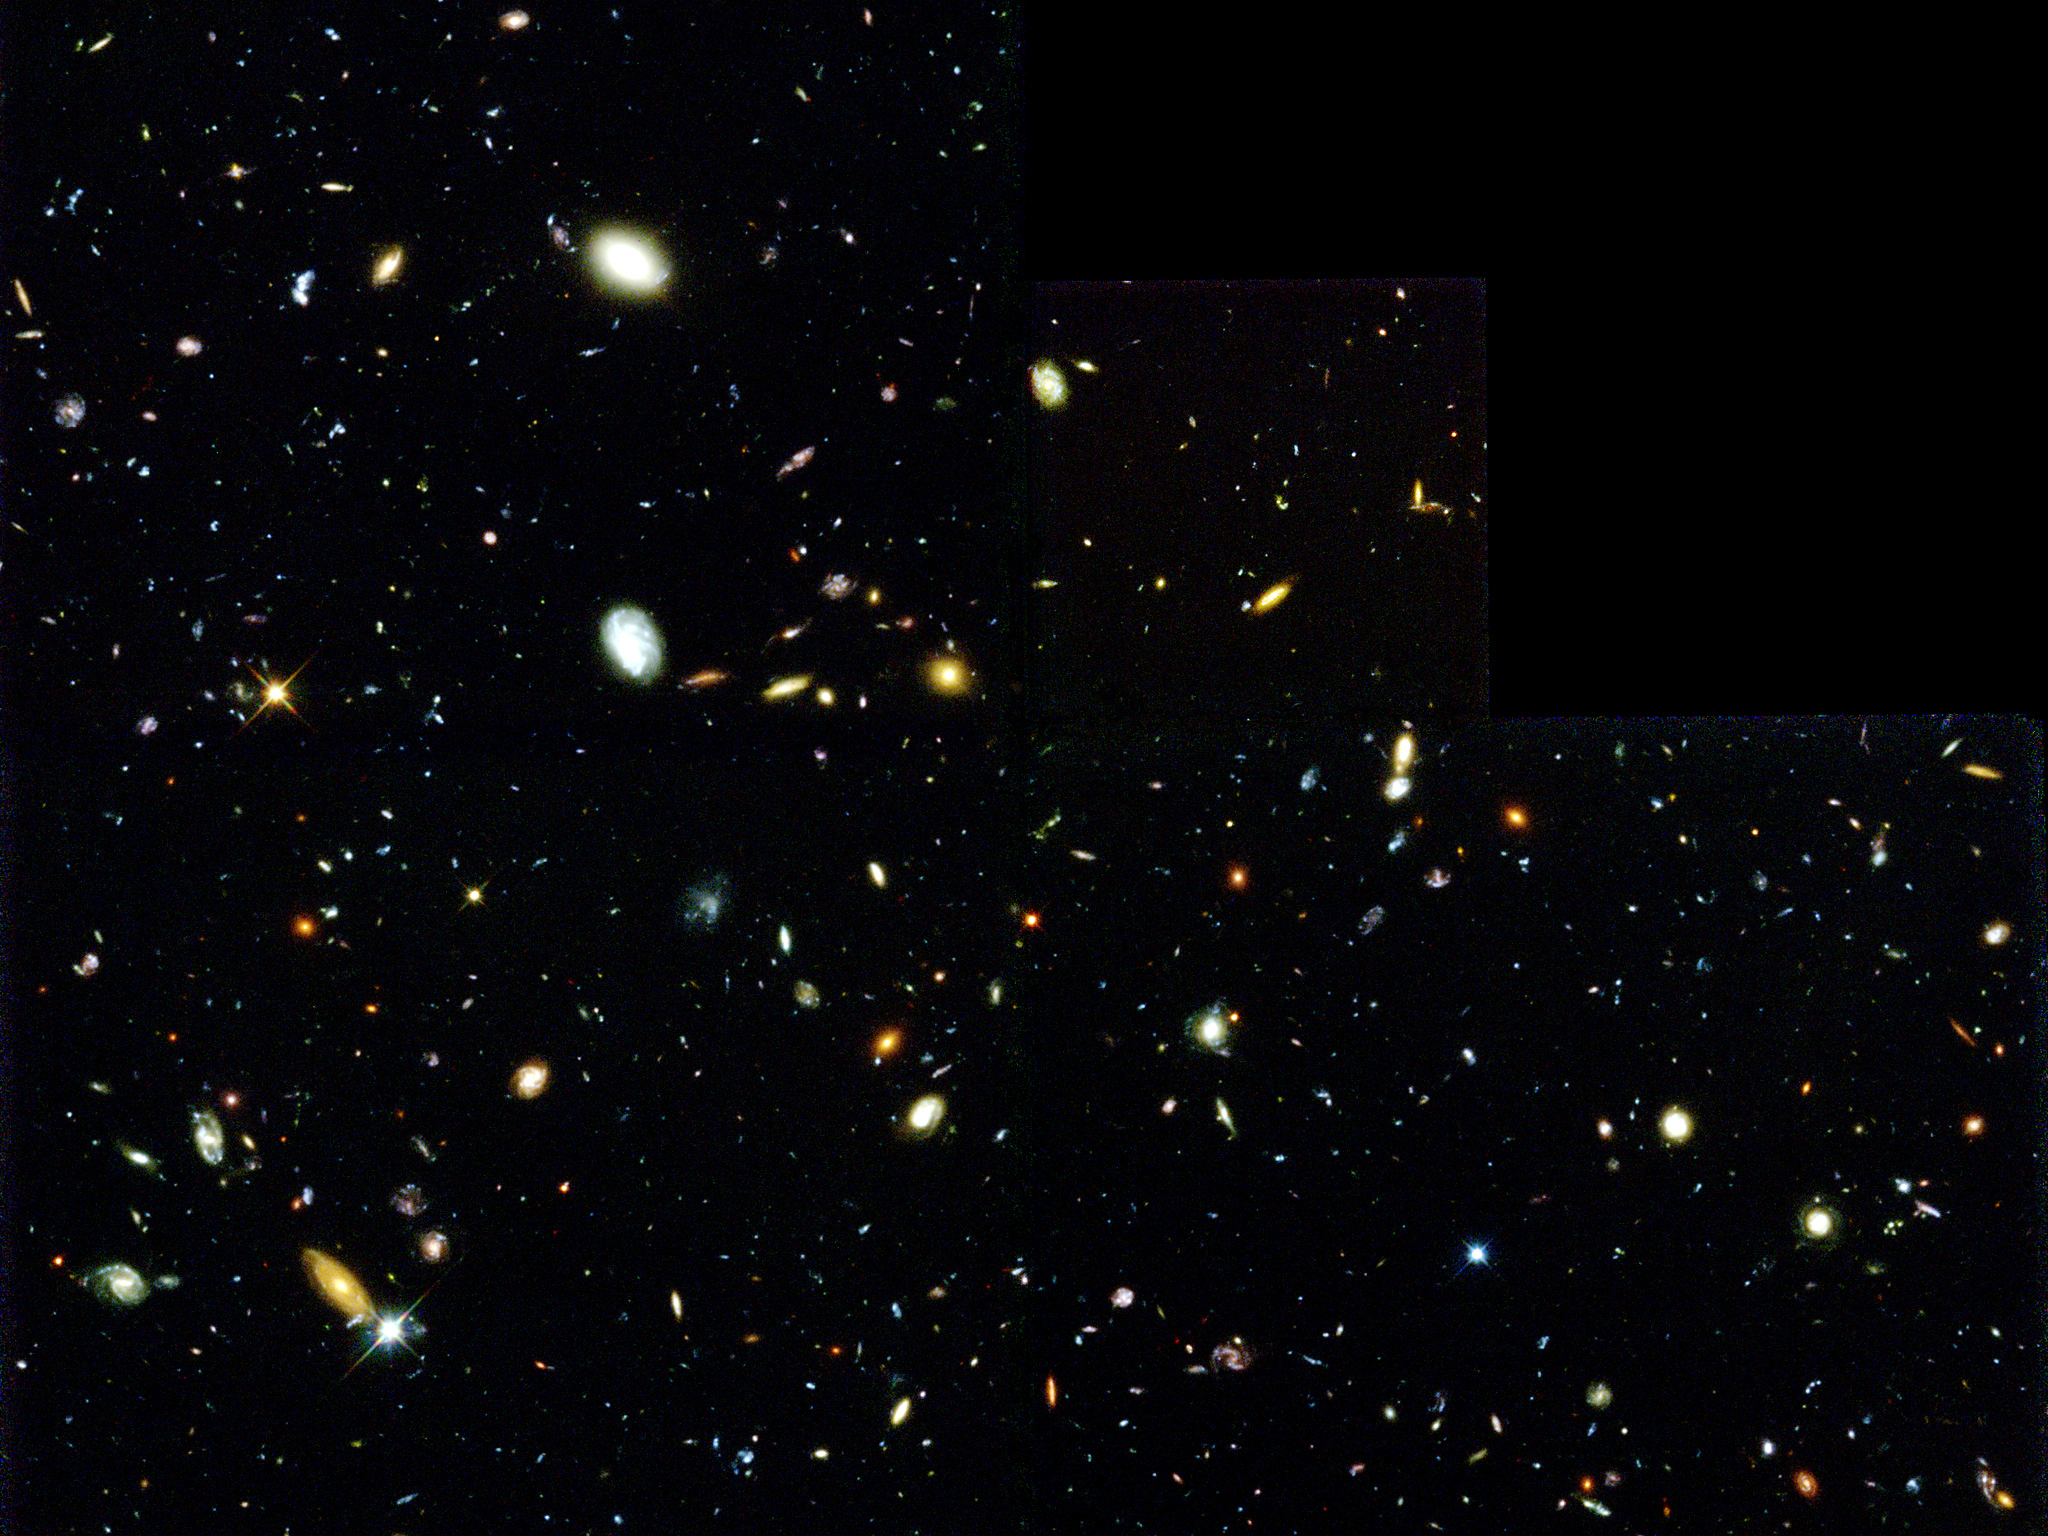
\includegraphics[width=0.9\columnwidth]{Figures/hubble_deep_field.jpeg}
	\caption{The Hubble Deep Field as captured by the Wide Field and Planetary Camera 2 onboard the \textit{Hubble Space Telescope} in 1995.}
	\label{fig:hubble_deep_field}
\end{figure}

\section{Galaxy Formation and Evolution}

To answer our questions on the evolution of galaxies, we must first make some inferences about the {\color{red}[...]} of the Universe. Our understanding of the cosmic history of galaxies is dependent on our choice of cosmology, which is widely accepted to be in the form of the $\Lambda$-CDM model (\citealt{Peebles_1980}). In the $\Lambda$-CDM model, Cold Dark Matter, matter of unknown origin, dominates over ordinary baryonic matter; and with dark energy, constitute a combined $\sim 95\%$ of the total cosmic energy budget (\citealt{Fukugita_2004}). The presence of dark matter is only evident in its gravitational interactions with other matter, but its origin is unknown as it does not interact with nor emit any electromagnetic radiation. The dark energy in the Universe is parameterized in the form of the cosmological constant, $\Lambda$, which is required to explain the accelerating expansion of the Universe. In this model, galaxy formation is seeded by small quantum fluctuations in the density of the early Universe, which grow with inflation to form small overdensities that later become the sites of dark matter halos by gravitationally attracting nearby dark matter. The first galaxies formed from these originally minute overdensities in density, which later merge due to an increase in collisions in a smaller Universe, to form ever larger galaxies. This model of galaxy formation is called a 'hierarchical' model, where galaxies in the early Universe are expected to be smaller and formed their mass more quickly than massive galaxies at later times that formed much of their stellar mass from previous mergers. As we shall show in Chapter \ref{chapter:Radio_Identifications}, this model of evolution may not explain the stellar build up of all galaxies.

\subsection{Classification of Galaxies}

The first step in understanding galaxy evolution by observing how galaxies have changed as we look back in time, is to classify galaxies according to their observable properties. Generally, galaxies can be classified into two broad groups based on their morphology: spirals and ellipticals. This dichotomy prompted the first classification scheme by Edwin Hubble (Figure \ref{fig:hubble_tuning_fork}; \citealt{Hubble_1936}), the \textit{Tuning Fork}, which shows ellitpical galaxies along the "handle", becoming more oblate towards the spiral galaxies. The spiral galaxies themselves are split into two categories forming the two "prongs", depending on the presence of a bar at the centre. At the join of the two, classified on the \textit{Tuning Fork} as S0, is where we might locate \textit{lenticular galaxies}, that are recognized by their large disks, like spirals, but without the presence of arms. In the rest of this Thesis we shall predominantly be referring to elliptical galaxies at \textit{early-type galaxies} (ETGs) and spiral-like galaxies as \textit{late-type galaxies} (LTGs), as is convention. Despite their names, the two do not represent a former and latter evolutionary stage of a typical galaxy, and is rather a misnomer. A minority of galaxies do not conform to this dichotomous image and are typically grouped together as \textit{irregular galaxies}.

\begin{figure}
    \centering
	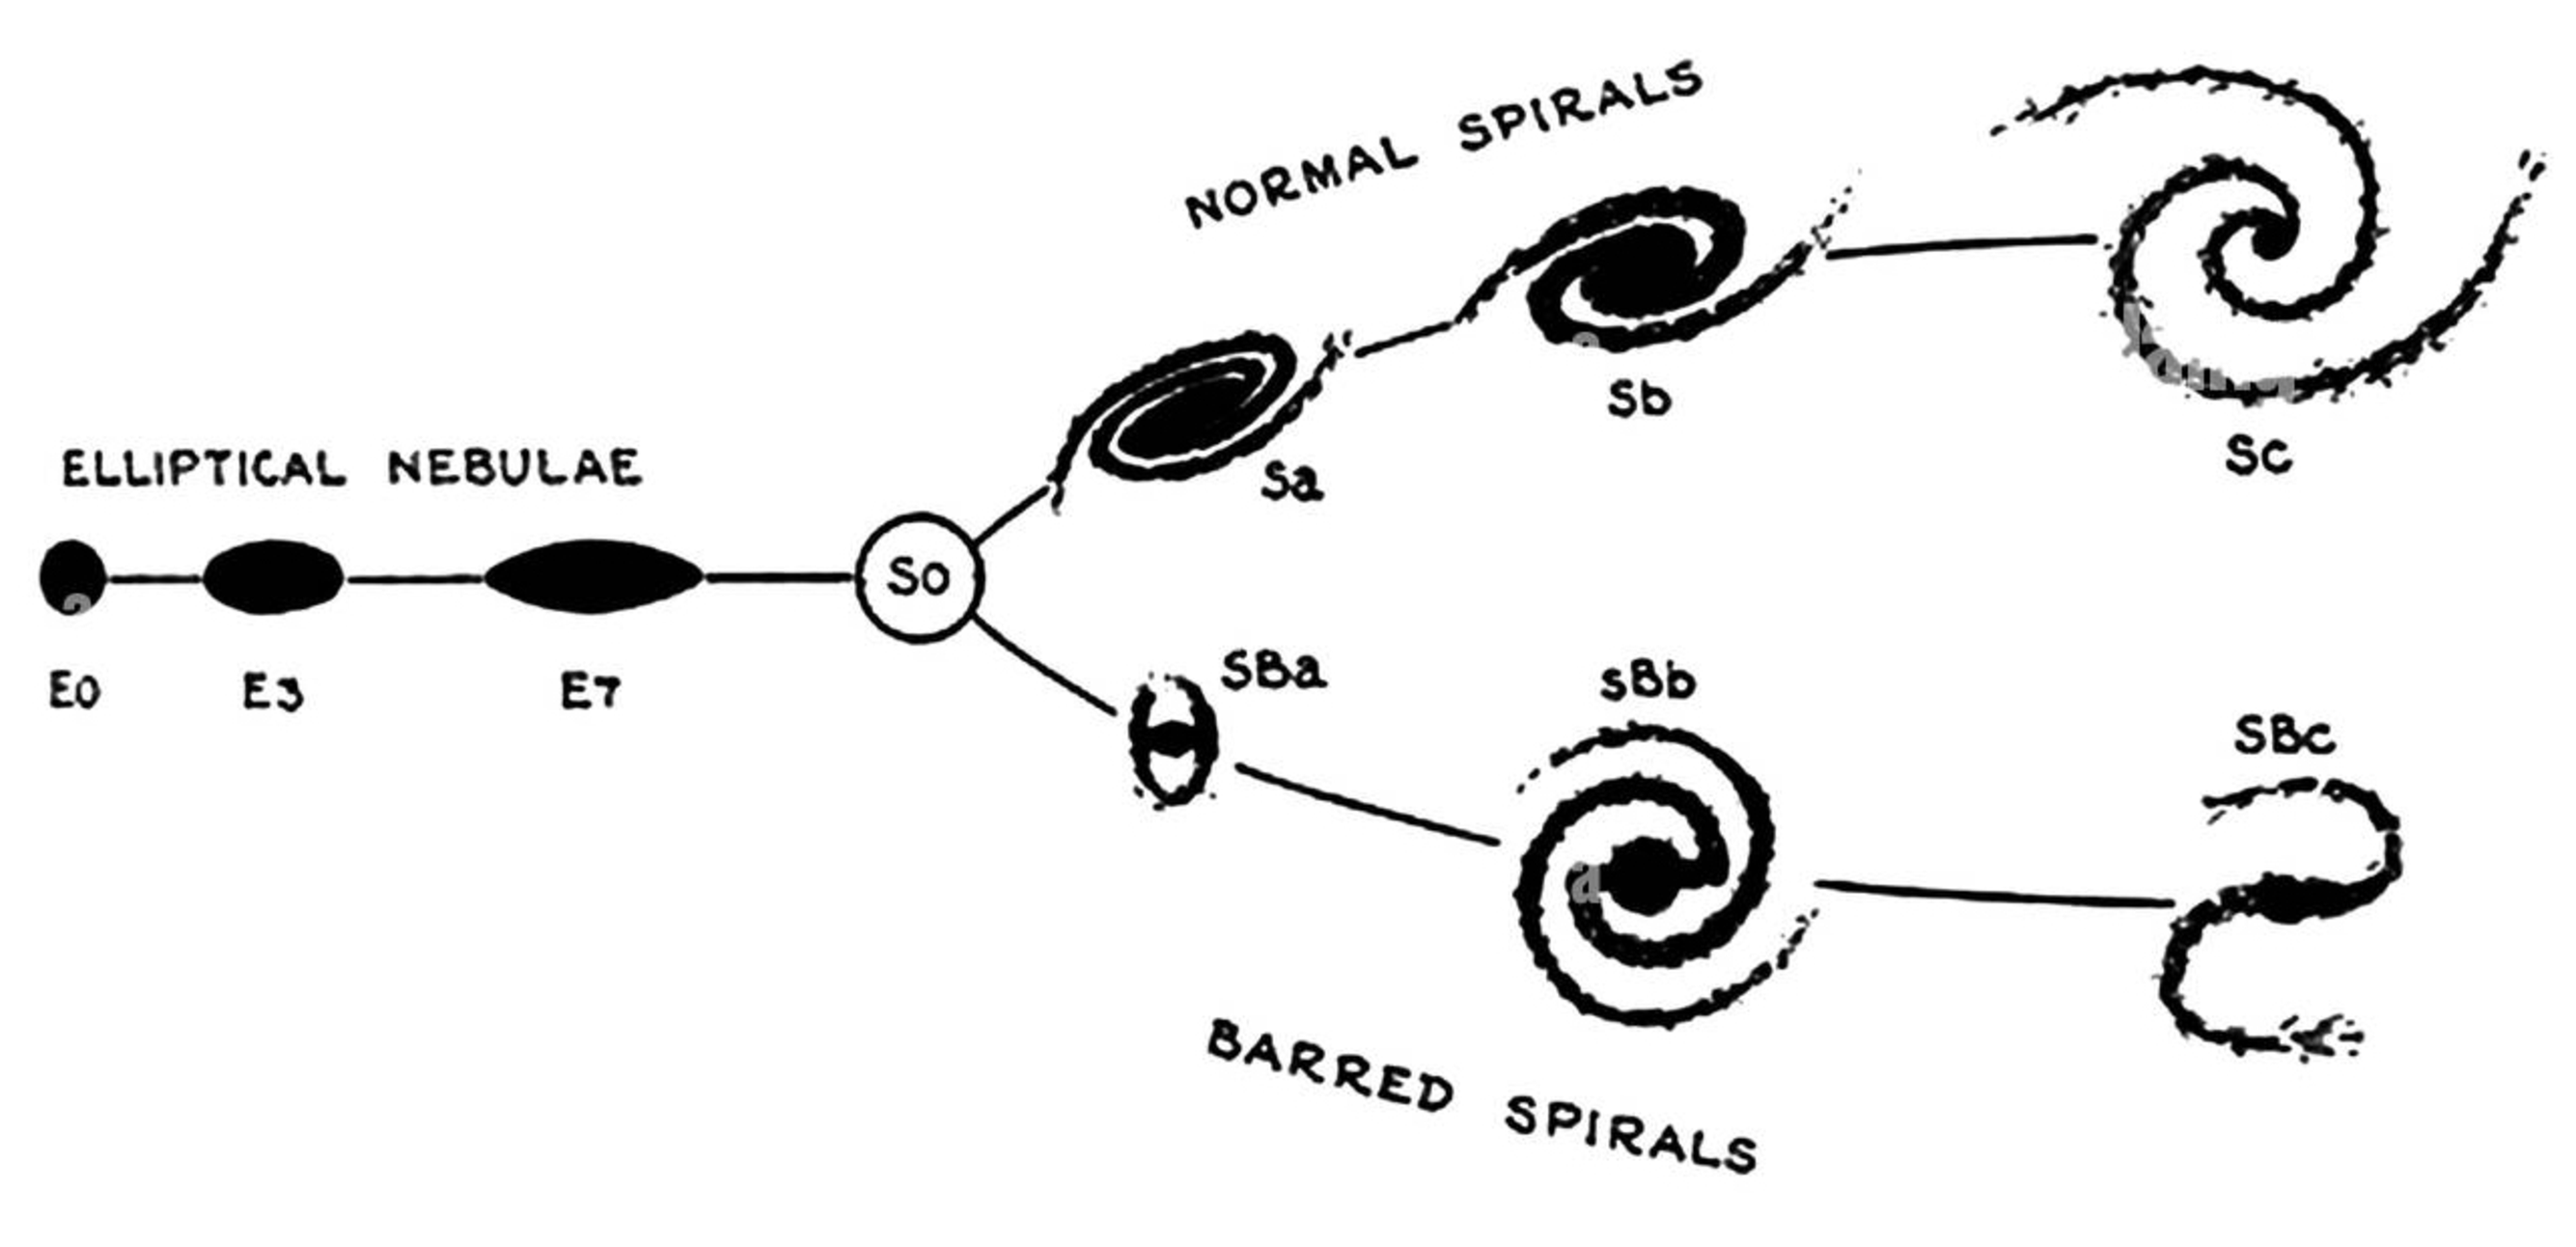
\includegraphics[width=0.9\columnwidth]{Figures/hubble_tuning_fork}
	\caption{The \textit{Hubble Tuning Fork}, or the \textit{Sequence of Nebular Types} as named in \citealt{Hubble_1936}, showing spiral galaxies along the prongs of the tuning fork and elliptical galaxies along the handle. The two prongs separate those spiral galaxies with barred central bulges from those that do not. Lenticular galaxies can be found at the join of the handle to the prongs. From left to right, the elliptical galaxies become more oblate and the spiral galaxies have spiral arms that become less tightly wound around the central bulge.}
	\label{fig:hubble_tuning_fork}
\end{figure}

Beyond their shape, the two broad groups, ETGs and LTGs, have a number of physical characteristics that are common to galaxies of the same class. First, the stellar populations of ETGs and LTGs are different. ETGs are dominated by old stellar populations that appear red in colour because they contain longer-lived, low mass stars, whereas LTGs typically have younger stellar populations of massive, but very short-lived stars.

ETGs are considered to be some of the most massive, luminous galaxies (due to having vast quantities of old stars) observed in the local Universe (\citealt{Bernardi_2003}; \citealt{Kelvin_2014}; \citealt{Moffett_2016}). Their stellar content is often centrally distributed, with the density of stars decreasing to the outskirts of the galaxy. In this central bulge of stars is where most of the interstellar medium (ISM) is located, though it is not expected to be substantial, and the limited amount of gas prohibits new star formation. In a hierarchical view of star formation, such ellipticals are formed from a series of major and minor mergers that consume the gas in the galaxy, leading to the quiescent systems observed today (\citealt{Toomre_1972}). In contrast, LTGs have dusty spiral arms with sites of active star formation, with older stars mainly located within the central bulge. While ETGs are largely devoid of gas, LTGs have a rich ISM that continues to fuel star formation, creating new stars at typical rates of several stars per year (\citealt{Kennicutt_1983}; \citealt{Gao_2004}). Our own Milky Way is an SBc spiral galaxy (\citealt{Gerhard_2002}) with active star formation at a rate of $\sim 2\,M_\odot$yr$^{-1}$ (\citealt{Noriega-Crespo_2013}; \citealt{Licquia_2015}; \citealt{Elia_2022} and references therein).

\subsection{The Star Forming Main Sequence}

A natural diagram to illustrate the difference in colour of ETGs and LTGs is to show the colours of optically-selected galaxies against their absolute magnitude. Galaxies discovered in optical surveys readily form two distinct regions: a \textit{red sequence} and a \textit{blue cloud}, with a sparsely populated region in between, the \textit{green valley}. Due to their optical colours, the red sequence is dominated by ETGs and the blue cloud dominated by LTGs. Moving away from observed quantities to intrinsic quantities, we note that the colour is a strong indicator of the star formation rate (SFR) in a galaxy and that absolute magnitude is approximately proportional to the size of the stellar population, and thus the stellar mass, $M_*$. In this formalism, the blue galaxies form a tight correlation known as the \textit{Main Sequence} (MS) or \textit{Star Forming Main Sequence}, while the red sequence occupies a \textit{passive cloud} (or "red and dead" or "quiescent") region that lies below the MS at lower star formation rates (\citealt{Noeske_2007}; \citealt{Daddi_2007}; \citealt{Elbaz_2007}; \citealt{Rodighiero_2011}). Figure \ref{fig:star_forming_main_sequence} shows the main sequence and passive clouds (grey contours) that form from the optically-selected Sloan Digital Sky Survey (SDSS; \citealt{York_2000}). \citealt{Saintonge_2017} present the \textit{Extended CO Legacy Database for GASS}, xCOLD GASS, a mass-selected sample from SDSS that have molecular gas mass estimates, which are plotted in colour in Figure \ref{fig:star_forming_main_sequence}. The molecular gas mass fraction, $f_{\textrm{H}_2} \equiv M_{\textrm{H}_2}/M_*$, clearly declines towards the passive cloud, showing the depleted ISM in ETGs.

{\color{red}Perhaps add a paragraph on the stellar-mass growth sequence, as illustrated by Figure 12 of Graham+2023}

\begin{figure}
    \centering
	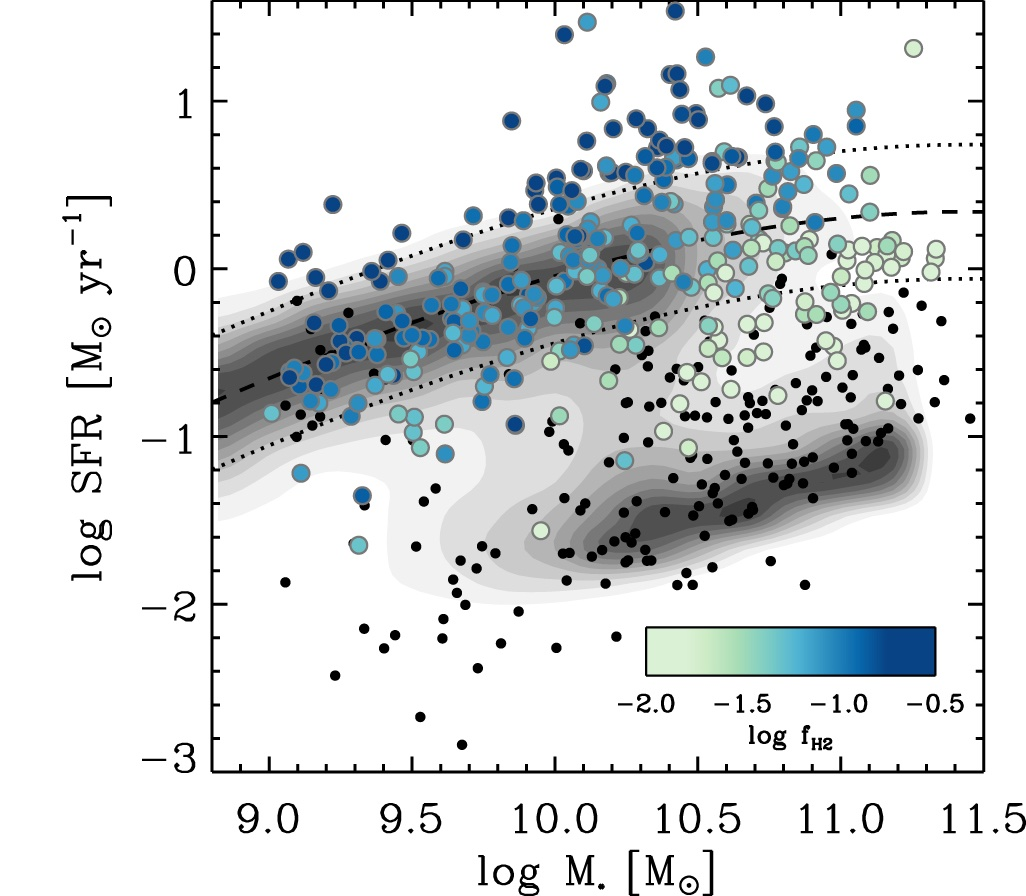
\includegraphics[width=0.75\columnwidth]{Figures/saintonge_ms.jpg}
	\caption{The distribution of SDSS galaxies in the SFR-$M_*$ plane (grey contours) from \citealt{Saintonge_2017} (Figure 7). The dashed line represents the location of the main sequence, while the dotted lines represent $\pm0.4\,$dex scatter around this relation. The coloured points show the distribution of galaxies from xCOLD GASS, coloured according to their molecular gas mass fraction.}
	\label{fig:star_forming_main_sequence}
\end{figure}

It is predicted that the vast majority, approximately $90\%$, of all cosmic star formation between redshifts $0$ and $2.5$ occurs in galaxies that reside on the MS, however, an important contribution also comes from galaxies that sit substantially above the relation. These galaxies, undergoing high levels of star formation for a short period of time, are collectively referred to as \textit{starburst galaxies} (e.g. \citealt{Muxlow_2006}; \citealt{Rinaldi_2022}). Starbursts form a small minority of galaxies, approximately $2\%$ of star forming galaxies depending on the exact definition of a starburst, but contribute $\sim 10\%$ of the cosmic star formation rate density (SFRD) at $z \sim 2$ (\citealt{Rodighiero_2011}), corresponding to the time in cosmic history when star formation was at its peak (see Section \ref{sec:cosmic_star_formation_history}).

Given that galaxies in the passive cloud have large stellar masses, they must have been at some point among the actively star forming galaxies, and then some process quench them of their star formation leading them to the passive cloud. The prevailing interpretation of the SFR-$M_*$ diagram is that a typical galaxy evolves along the sequence, gaining stellar mass, increasing their star formation rate accordingly and depleting the gas available for star formation in the process. At some point, the galaxy stops forming stars entirely, and falls off the main sequence. The valley between the MS and the passive cloud, a result of a dearth of galaxies in this regime, suggests that the quenching process that turns off the star formation in the galaxy is fast. This image of galaxy evolution, however, is not without scepticism. Recent studies (e.g. \citealt{Eales_2018}; \citealt{Bremer_2018}; \citealt{Phillipps_2019}) have suggested that the bimodal distribution of star forming and passive galaxies may be a reflection of selection effects in optical surveys, prompting attempts to define the whole population of galaxies using a probability distribution with only one maximum (e.g. \citealt{Corcho-Caballero_2020}). {\color{red}Explain the evidence for an apparent bimodality (Read abstracts of three papers above - that is all that is needed.)}

Whether there are two distinct classes or whether the transition between morphological types and physical properties is gradual, some physical process must be coverting a star forming galaxy on the MS to one that is passive, quenching it of star formation. There are many possibilities that have been proposed as the cause of quenching, and it is likely that all are important in different scenarios. These processes include stellar feedback and winds from supernovae removing the gas from a galaxy (\citealt{Hayward_2017}); gas expulsion by active galactic nuclei, AGN (\citealt{Springel_2005}; \citealt{Croton_2006}; \citealt{Cicone_2014}; \citealt{Harrison_2017}); the formation of a galactic bar or central bulge (\citealt{Bournaud_2007}; \citealt{Martig_2009}) which relocates the gas to the galactic center and reduces the star formation in the disk, as well as a range of environmental processes such as galaxy merging (\citealt{Lavery_1994}; \citealt{Weigel_2017}) which ignites a starbursting phase that rapidly consumes the gas; ram-pressure stripping, the loss of gas as the galaxy passes through the intra-cluster medium (\citealt{Gunn_1972}; \citealt{Boselli_2006}; \citealt{Domainko_2006}; \citealt{Boselli_2014}), and quenching mechanisms that result from being in high density environments such as galaxy clusters, like galaxy harassment and strangulation (\citealt{Moore_1996}; \citealt{Moore_1998}; \citealt{Bekki_2002}).

\subsection{Cosmic Star Formation History}
\label{sec:cosmic_star_formation_history}

We have seen that the star formation rates of galaxies is intrinsically linked to its evolutionary stage, and thus it would be unsurprising to identify an evolution in the integrated SFRs of galaxies with cosmic time. By measuring the star formation of many galaxies at different epochs, we can build a picture of the star formation density in the Universe. The cosmic history of star formation is one of the fundamental observables of astronomy, giving us an insight into the timeline for which gas forms into stars, heavy elements are produced (elements heavier than the primordial hydrogen and helium are produced in stars), and dust is formed (as dust is a natural byproduct of star formation, see Section {\color{red}X}).

The cosmic star formation rate density (SFRD {\color{red}Repeated}) in the Universe can be estimated in two ways. The most straightforward way to estimate the star formation rate is to measure the amount of starlight we observe from tracers of recent star formation in galaxies. In this sense, the SFR indicator should be sensitive to the short-lived massive stars at each point in cosmic history, and thus the UV and optical stellar light is often used (e.g. \citealt{Madau_1996}; \citealt{Lilly_1996}; \citealt{Wyder_2005}; \citealt{Schiminovich_2005}; \citealt{Dahlen_2007}; \citealt{Reddy_2009}; \citealt{Robotham_2011}; \citealt{Cucciati_2012}; \citealt{Schenker_2013}; \citealt{Finkelstein_2015}). Second, we note that approximately half of all optical and UV light from stars ever emitted in the Universe has been absorbed by dust and re-emitted at far-infrared (FIR) and sub-millimeter (sub-mm) wavelengths (\citealt{Puget_1996}; \citealt{Fixsen_1998}; \citealt{Dole_2006}; \citealt{Driver_2008}; \citealt{Driver_2016}). This means that a significant contribution to the SFRD must also be measured from far-IR/sub-mm indicators of star formation that probe the stellar light reprocessed by dust (e.g. \citealt{Magnelli_2011}; \citealt{Casey_2012}; \citealt{Magnelli_2013}; \citealt{Gruppioni_2013}; \citealt{Swinbank_2014}; \citealt{Bouwens_2016}; \citealt{Bourne_2017}; \citealt{Koprowski_2017}; \citealt{Novak_2017}; \citealt{Liu_2018}; \citealt{Bouwens_2020}; \citealt{Dudzeviciute_2020}).

{\color{red}Rewrite above as it is not strictly two separate ways. See Wise+2023.}

Figure \ref{fig:cosmic_sfrd} shows that the dust-obscured and unobscured measures of the SFRD have peaks at $z\sim2$ (when the Universe was roughly 3 billion years old), followed by a slow decline by a factor of $\sim 8$ to the present day. The short period corresponding to the peak of star formation is often referred to as \textit{cosmic noon}. In the (approximate) 3.5\,Gyr between $z\sim3$ and $z\sim1$, spanning cosmic noon, up to half of the stellar mass we observe today was formed (\citealt{Forster-Schreiber_2020}). The galaxies that are identified at these redshifts are ideal targets for tracing the formational epoch of the massive LTGs and ETGs seen in the local Universe. We see that most of the star formation at $z < 3$ is obscured by dust and even at higher redshifts the contribution appears significant. The FIR and sub-mm traced component has dominated the cosmic history of star formation for the past $\sim 12\,$Gyr, contributing approximately $80\%$ of the total star formation. The top panel of Figure \ref{fig:cosmic_sfrd} shows the contribution from galaxies with different IR luminosities to the dust-obscured star formation. It is clear that massive, IR luminous galaxies dominate the star formation history at earlier times. At this point, we clarify some acronynms commonly used to refer to bright infrared galaxies (the IR luminosities of galaxies are assumed to be the bolometric luminosity integrated between $8$ and $1,000\,\mu$m):

\begin{itemize}
    \item Luminous Infrared Galaxy (LIRG) - Defined as having $10^{11} < L_\textrm{IR} [L_\odot] < 10^{12}$.
    \item UltraLuminous Infrared Galaxy (ULIRG) - Defined as having $10^{12} < L_\textrm{IR} [L_\odot] < 10^{13}$.
    \item HyperLuminous Infrared Galaxy (HyLIRG) - Defined as having $L_\textrm{IR} [L_\odot] > 10^{13}$.
\end{itemize}

\begin{figure}
    \centering
	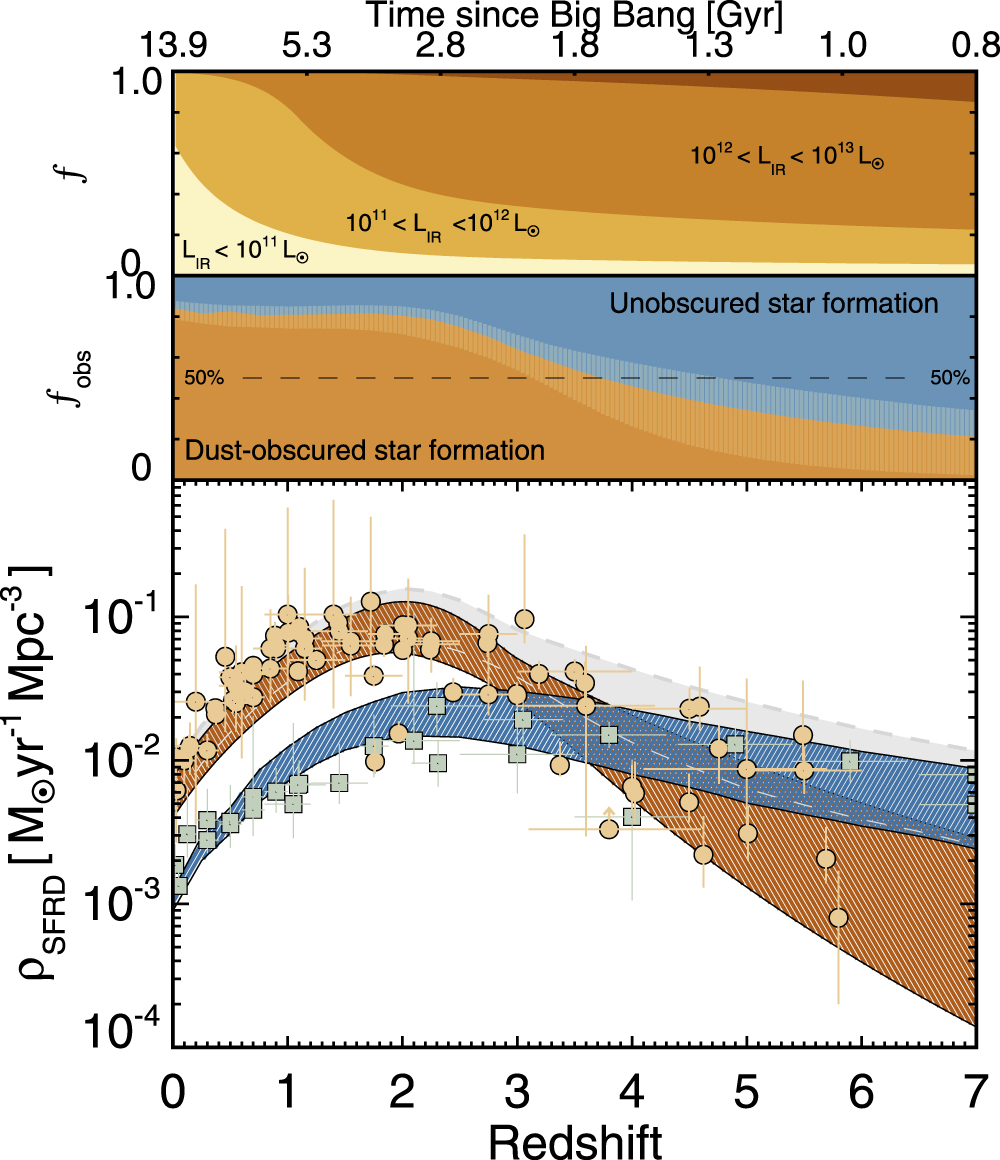
\includegraphics[width=0.75\columnwidth]{Figures/cosmic_sfrd.jpeg}
	\caption{The cosmic star formation history from \citealt{Zavala_2021}. The contributions to the total star formation rate density (grey) from dust-obscured IR/sub-mm surveys and from unobscured UV/optical surveys are shown in orange and blue, respectively. The top panel shows the contribution from galaxies with different IR luminosities to the dust-obscured SFRD. The classes shown are $L_\textrm{IR} < 10^{11}\,L_\odot$, $10^{11} < L_\textrm{IR} [L_\odot] < 10^{12}$ (LIRGs) and $10^{12} < L_\textrm{IR} [L_\odot] < 10^{13}$ (ULIRGs). The middle panel represents the fraction of SFRD that is dust-obscured.}
	\label{fig:cosmic_sfrd}
\end{figure}

Looking back to cosmic noon, much of the star formation within dusty galaxies is happening in ULIRGs, while the integrated dust-obscured star formation begins to fall. This suggests that the number of massive galaxies declines at higher redshifts. Particularly at high redshifts ($z \gtrsim 3$), the exact amount of dust-obscured star formation is still uncertain. Large samples of galaxies with measured dust emssion are therefore required to elucidate our view on the cosmic history of star formation.

\section{The Interstellar Medium}

The interstellar medium (ISM) refers to the matter that fills the space in between the stars of a galaxy. It is the medium in which stars are born, and latter replenished with enriched material when they die. The matter comes in the form of gas - in ionic, atomic and molecular forms - and dust, in overwhelming favour of gas which constitutes $\sim99\%$ of the ISM, and dust the other $1\%$ ({\color{red}REFERENCE}). By mass, the gas in the ISM is around $70\%$ hydrogen, $28\%$ helium and $2\%$ heavier elements, reflecting only a small change from the ratios of the primordial matter created after the Big Bang (\citealt{Klessen_2016}). In terms of volume, most of the ISM is occupied by ionized gas, but due to its incredibly low volume density, only accounts for around $25\%$ of the gas mass. Most of the gas mass in a galaxy is in the form of neutral atomic gas (H and He) or molecular (H$_2$) and can be found in dense clouds that take up only $1-2\%$ of the total volume of the ISM.

The ISM spans a wide range of temperatures and densities, leading to many interpretations of the ISM as being in distinct phases, despite there being no obvious separation between different phases (\citealt{Cox_2005}). A two phase model was proposed by \citealt{Field_1969}, showing that atomic gas in the ISM can exist at two stable temperatures. These two solutions correspond to cold and dense gas at $T\sim100\,$K and warm, diffuse gas at $T\sim10^4\,$K. These are now referred to as the Cold Neutral Medium (CNM) and Warm Neutral Medium (WNM), respectively. This model was extended to three phases by \citealt{McKee_1977}, who noted that supernovae in the ISM creates bubbles of very hot, ionized gas ($T\sim10^6\,$K). This phase of the ISM is known as the Hot Ionized Medium (HIM). A cooler, Warm Ionized Medium (WIM) has a temperature and density similar to the WNM, but contains around $90\%$ of the ionized gas in the ISM (\citealt{Haffner_2009}). A final distinction is typically made for the molecular clouds that are cold, but distinctly more dense than the CNM. The molecular gas clouds have a range of masses and sizes, and is known to correlate with observed star formation in the Galaxy. The approximate temperatures, densities, mass fractions and volume filling fractions of the phases in the ISM for a dynamic spiral galaxy is given in Table \ref{tab:ISM_phases} as presented in \citealt{Ferriere_2001} and {\color{red}Walter?}. The fractions are highly uncertain but represent what might be realistic estimates for a spiral galaxy containing all five phases of this model of the ISM.

\begin{table}
	\centering
	\begin{tabular}{p{4cm}|p{3cm}|p{3cm}|p{1.5cm}|p{1.5cm}}
		\hline
		\hline
		Phase & T [K] & $n$ [atoms cm$^{-3}$] & $f_{\textrm{Mass}}$ & $f_{\textrm{Volume}}$ \\
		\hline
		\hline
		Molecular Clouds & $10 - 20$ & $>10^2$ & $\sim 20\%$ & $<1\%$ \\
		Cold Neutral Medium & $50 - 100$ & $20 - 50$ & $\sim 40\%$ & $\sim2 - 4 \%$\\
		Warm Neutral Medium & $6,000 - 10,000$ & $0.2 - 0.5$ & $\sim 30\%$ & $\gtrsim 30\%$ \\
		Warm Ionized Medium & $\sim8,000$ & $0.2 - 0.5$ & $\sim 10\%$ & $\gtrsim 15\%$ \\
		Hot Ionized Medium & $\sim10^6$ & $\sim10^{-2}$ & $\sim 1\%$ & $\lesssim 50\%$ \\
		\hline
	\end{tabular}
	\caption{The different phases of the ISM and their expected temperatures, densities, mass fractions and volume filling factors.}
	\label{tab:ISM_phases}
\end{table}

This multi-phase picture is certainly an oversimplification of the conditions found in the ISM. The ISM is shaped by a variety of processes that blur the distinction between these distinct phases. The actual ISM is continuous and dynamic with transitional regions between the phases. Processes that contribute to the blurring of the boundaries between different phases include turbulence from supernova shocks (\citealt{MacLow_2004}) and stellar winds, thermal instability (\citealt{Kritsuk_2002}) and the presence of magnetic fields.

Figure \ref{fig:interstellar_medium} shows various components of the ISM in the Galaxy, as traced by different wavelengths of the electromagnetic spectrum. The top two panels highlight the starlight that is observable at optical ($0.5\,\mu$m) and near-infrared ($2\,\mu$m) wavelengths. The stellar light is blocked by dust in the optical image, whereas the near-infrared clearly shows the stellar distribution, making the dark dust clouds appear almost transparent. The benefit that the infrared provides in identifying the stellar light of a galaxy, compared to optical wavelengths, is a key motive for the studies presented in Chapters \ref{chapter:Data_Release_3} and \ref{chapter:Dust_Mass_Functions}. As we traverse the electromagnetic spectrum to the far-infrared (third panel, observed at $350\,\mu$m) the emission from the dust itself becomes visible. The final three panels show the emission from atomic, ionized and molecular gas in the Galaxy. The atomic gas is traced by the $21\,$cm spectral line, originating from the hydrogen \textit{spin-flip} transition between a proton-electron aligned state to an anti-aligned state. This transition is forbidden - the mean lifetime of a hydrogen atom being in the excited, aligned state is approximately 11 million years ({\color{red}REFERENCE}) - meaning that the likelihood of the transition is incredibly rare. However, as can be seen in the figure, the abundance of atomic hydrogen means that the $21\,$cm line is a useful tracer for gas in the ISM. The limitation of the $21\,$cm line is that it is only useful for tracing the distribution of neutral hydrogen in the local Universe where the emission is still strong enough to be detected. The $74\,$cm radio emission in the penultimate panel traces the radiation from ionized gas. The radio emission emanates from accelerated charged particles, which may be observed in HII regions and supernova remnants. The final panel shows the molecular gas phase, as traced by the $2.6\,$mm spectral line of carbon monoxide (CO). As will be detailed later, the rotational transitions of the CO molecule is a useful tracer of dense molecular regions, and it is often assumed that wherever there are CO molecules there must also exist H$_2$ molecules. This map shows the locations of cold gas in the Galaxy and the sites of star formation.

\begin{figure}
    \centering
	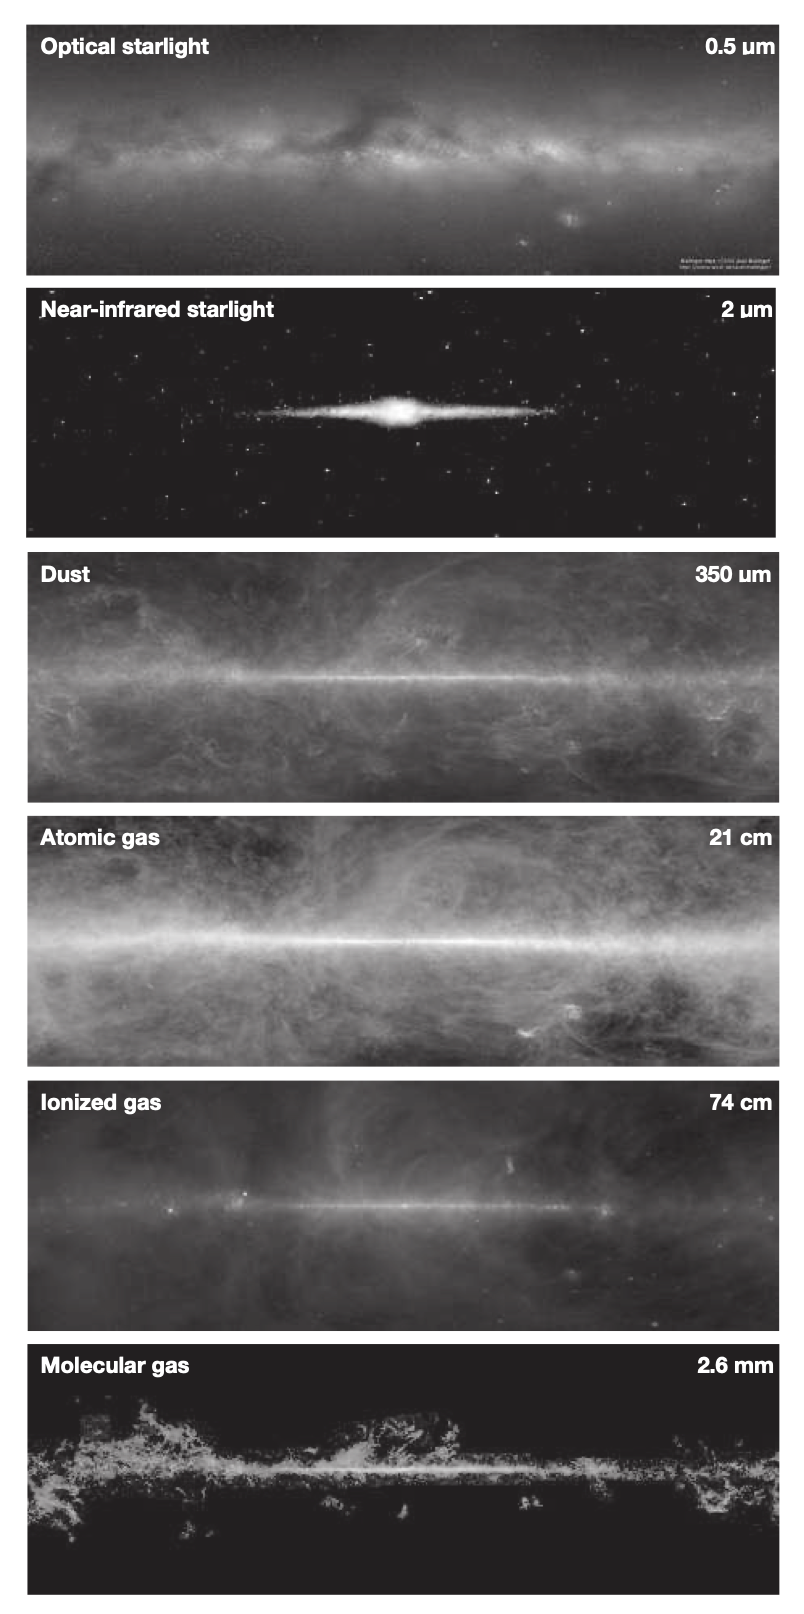
\includegraphics[width=0.75\columnwidth]{Figures/interstellar_medium.png}
	\caption{{\color{red}Caption.} \citealt{Williams_2021}}
	\label{fig:interstellar_medium}
\end{figure}

A fundamental assumption that is made throughout this Thesis is that we can trace the hidden star formation in a galaxy via the dust emission observed in the far-IR and sub-mm wavelengths (as discussed in the following section). Figure \ref{fig:interstellar_medium} shows that the dust and gas are well mixed in the ISM of the Galaxy, and in Section \ref{sec:dust_tracing_star_formation} we describe how dust is an integral part of the star formation process in galaxies. As such, this assumption appears to hold and we may study the dust content of galaxies, and make inferences about their star formation, from the radiation emitted at far-IR and sub-mm wavelengths.

\section{Cosmic Dust}

\subsection{Chemical Composition and the Reprocessing of Starlight}

Cosmic dust is a general term that refers to the solid particles that exist in the ISM. These interstellar grains can have a range of sizes between $\sim 10\,$nm and $\sim 1\,\mu$m (\citealt{Kim_1994}; \citealt{Galliano_2018}) and are mostly composed of carbonaceous materials (materials that are predominantly Carbon by mass) and silicates. The larger dust grains are primarily silicates and amorphous carbon, which are the prime candidates for the dust grains that absorb UV and optical starlight and reradiates this energy in the far-IR and sub-mm regimes. Hydrogenated carbonaceous materials, like Polycyclic Aromatic Hydrocarbons (PAHs), are chemical compounds comprised of carbon and hydrogen molecules and are also {\color{red}[...]} interstellar dust grains. These molecules are the cause of strong spectral lines that can be observed in the mid-infrared (\citealt{Tielens_1987}; \citealt{Draine_2007a}; \citealt{Draine_2007b}).

The presence of dust along the line of sight to a population of stars can have several consequences on the emission that is observed. First, if the dust is thick enough, any background stellar light may not be visible at all, as is the case with some dark nebulae in the Galaxy such as the \textit{Horsehead Nebula}. For less opaque dust clouds, the light passing through can be dimmed due to the effects of dust extinction. This refers to the amount of background light that is absorbed and scattered out of the line of sight to the observer. The dimming effect is dependent on several factors including the density of the dust cloud, the grain size distribution and the wavelength of the light. More generally, dust attenuation refers to the effect on the spectrum of a background object as a result of dust, which includes dust extinction, but also includes scattering back into the line of sight and the light from unobscured stars. It is the attenuated stellar emission that is observed as a strong peak in the far-IR region of a galaxy's spectral energy distribution (SED). Figure \ref{fig:unattenuated_attenuated_sed} shows the UV to far-IR SED of NGC337, modelled using \texttt{MAGPHYS} (\citealt{daCunha_2008}), which illustrates how the true stellar spectrum of a galaxy (blue) is attenuated by dust to produce the far-IR emission (green) and the observed UV to far-IR spectrum (black). Moreover, interstellar dust is more efficient at absorbing and scattering blue light compared to red light, meaning that background stars behind a cloud of dust often appear more red than they are. This effect is known as interstellar reddening and can be observed in the spectrum of NGC337 - the shorter the wavelength (towards the blue end of the spectrum), the greater the difference between the attenuated and unattenuated stellar spectra.

\begin{figure}
    \centering
	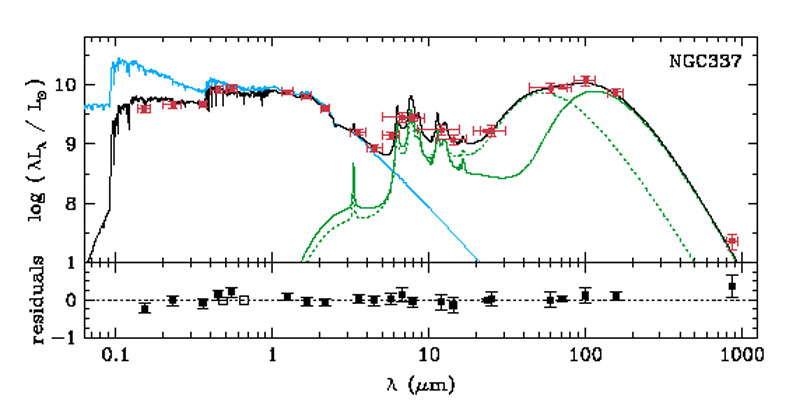
\includegraphics[width=0.9\columnwidth]{Figures/unattenuated_attenuated_sed.jpeg}
	\caption{{\color{red}Caption.} \citealt{daCunha_2008}}
	\label{fig:unattenuated_attenuated_sed}
\end{figure}

\subsection{The Lifecycle of Dust}

The lifecycle of dust grains, the mechanisms in which they are produced and destroyed, are important in understanding the metal enrichment and stellar evolution of galaxies. Dust can form in a number of ways including in the stellar winds of evolved stars, from the ejecta of supernovae or they can form in situ in the ISM (\citealt{Draine_2009}). Traditionally, the majority of dust was presumed to be formed in the outer envelopes of latter stage stars, such as red giant branch (RGB) and asymptotic giant branch (AGB) stars. These stars have masses of $1 < M_\textrm{star} [M_\odot] < 8$ and are in a late phase of evolution, having left the (stellar) main sequence and formed heavy elements. The metals solidify into grains in the envelopes of RGB and AGB stars and are carried out in the stellar wind and deposited into the ISM ({\color{red}REFERENCE}). For more massive stars with $M_\textrm{star} > 8\,M_\odot$, dust can form in the ejecta of {\color{red}[...]} supernovae, condensing from the leftover expanding material. The problem with this pathway, however, is that the dust yields from a single supernova are still a matter of debate, with studies observing dust masses in supernova remnants between roughly $0.05\,M_\odot$ and $1\,M_\odot$ (\citealt{Rho_2008}; \citealt{Dunne_2009}; \citealt{Barlow_2010}; \citealt{Matsuura_2011}; \citealt{Gomez_2012}; \citealt{Matsuura_2015}; \citealt{Chawner_2019}). Much of this debate is due to questions about how dust formed in supernovae may survive the destructive shock waves that are produced (\citealt{Draine_1979}; \citealt{Jones_1996}). The production rate of dust is a key open question, particularly for studies in the early Universe where a \textit{Dust Budget Crisis} has been proposed (e.g. \citealt{Dwek_2007}; \citealt{Michalowski_2010}; \citealt{Valiante_2011}). This refers to the difficulty in explaining the high dust masses observed in high redshift galaxies from dust produced via the Low-Intermediate Mass Stars (LIMS). Above redshifts $\sim 5$, there is little time for significant amounts of dust to be produced from the post main-sequence evolution of LIMS (\citealt{Morgan_2003}; \citealt{DiCriscienzo_2013}). The final production mechanism we mention here is dust formed in situ via grain growth. This method is most effective in the dense ISM, and so is particularly important in molecular clouds. Grain growth occurs when the conditions allow for the grains to form mantles of ice, which allow metals to subsequently stick to the grains (coagulation, \citealt{Blain_2004}).

We have mentioned one way in which dust can be destoyed in the ISM, via supernova shocks, but a second process contributing to dust destruction is \textit{sputtering}. Sputtering occurs as the result of the bombardment of gas atoms in dense environments causing the sublimation of the dust grains (\citealt{Barlow_1978}; \citealt{Jones_2004}).

\subsection{Dust Emission as a Tracer of Obscured Star Formation}
\label{sec:dust_tracing_star_formation}

Despite accounting for only $1\%$ of the ISM, interstellar dust plays an important role in the processes that govern the formation and evolution of galaxies.

{\color{red}I don't know what to write here: i) Sites of H2 formation?}

\section{Observing Dusty Star Forming Galaxies in the Far-IR and Sub-mm}

It is at this point that we find it useful to define approximate boundaries between different wavelength regimes of interest when talking about dust emission.{\color{red}[...]}

The majority of the dust in the ISM by mass has temperatures of roughly {\color{red} $X - X\,$K} ({\color{red}REFERENCES}). It is the thermal emission from this cool dust that we observe in the far-IR and sub-mm regimes. As can be seen in the example SED of Figure \ref{fig:unattenuated_attenuated_sed}, the dust emission creates a steep sub-mm spectrum. 

[Observations in this regime probe most of the dust in the ISM]



\chapter{Herschel-ATLAS Data Release III}
\label{chapter:Data_Release_3}
[...]\todo[color=red]{A brief introduction to the chapter.}

\section{The Herschel-ATLAS}
\label{sec:The Herschel-ATLAS}

The \textit{Herschel} Astrophysical Terahertz Large Area Survey (H-ATLAS; \citealt{Eales_2010}) was the largest open-time sub-mm survey carried out with \textit{Herschel}. The survey was observed across five photometric bands using two instruments onboard the \textit{Herschel Space Observatory}: the Photodetector Array Camera (PACS, \citealt{Poglitsch_2010}) at 100 and 160\,\micron, and the Spectral and Photometric Imaging Receiver (SPIRE, \citealt{Griffin_2010}) at 250, 350 and 500\,\micron. Compared to the first SMGs detected using SCUBA at 850\,\micron (\citealt{Smail_1997}; \citealt{Barger_1998}; \citealt{Hughes_1998}), the PACS and SPIRE wavebands span the peak of the infrared spectrum for low redshift (z < 1) galaxies. Their intrinsic brightness at the SPIRE wavelengths makes their detection in the thousands more achievable. The main scientific goal of the survey was to estimate the dust masses and dust obscured star formation rates for thousands of nearby galaxies over a large area of sky. While the intention was for a shallow survey, the surprising sensitivity of \textit{Herschel} and the negative k-correction observed at the operating wavelengths of the SPIRE instrument (\citealt{Blain_1993}) means that many sources were observed at higher redshifts, with a median of z $\sim$ 1. The catalogues of the survey, as detailed below, includes sources with redshifts up to $\sim$ 6 (\citealt{Amblard_2010}; \citealt{Lapi_2011}; \citealt{Fudamoto_2017}; \citealt{Zavala_2018}).

The complete survey covers $\sim$\,660\,$\deg^2$, split into three regions located to avoid emission from Galactic dust and to utilize complimentary spectroscopic surveys including the Sloan Digital Sky Survey (SDSS, \citealt{York_2000}), the 2df Galaxy Redshift Survey (2dfGRS, \citealt{Colless_2001}) and the Galaxy and Mass Assembly (GAMA, \citealt{Driver_2009}). The North Galactic Pole (NGP) region covers $\sim$\,180\,$\deg^2$ of the northern sky, centered at R.A 13$^{h}$18$^{m}$ and declination +29$^{\circ}$13' (J2000); three equatorial fields, located at approximately R.A 9$^{h}$, 12$^{h}$ and 15$^{h}$ coinciding with the GAMA survey (henceforth named GAMA9, GAMA12 and GAMA15 fields), each with an area of approximately 54\,$\deg^2$, and the South Galactic Pole (SGP) region, centered at R.A 0$^{h}$6$^{m}$ and declination -32$^{\circ}$44' (J2000) with an area of $\sim$ 318\,$\deg^2$. 

\subsection{Detecting Submillimeter Sources on Herschel Images}
\label{sec:Detecting Submillimeter Sources on Herschel Images}

Due to [...]\todo[color=orange]{continuation:} sub-mm images suffer from two types of noise; instrumental noise [...]\todo[color=orange]{continuation:} and confusion noise which is highly correlated between pixels, most of its contribution coming from the blending together of faint sources. Source confusion is of particular importance to sub-mm surveys [...]\todo[color=orange]{continuation:}. The result of combining instrumental noise with confusion noise is that almost all sources in the Herschel images are unresolved and the optimum filter for detecting these unresolved sources is no longer the point spread function (PSF). Consider a \textit{Herschel} map in which there is only one source of noise: an image with instrumental noise but no confusion noise (i.e. there is only one point source and no fainter, confusing sources), the optimal detection of this source is obtained by convolving the image with the PSF of the instrument. On the other hand, a map with no instrumental noise, but many confused point sources would be optimally detected with its best signal to noise ratio (SNR) by taking the Fourier transform of the image, dividing by the Fourier transform of the PSF and taking the inverse Fourier transform to obtain a perfect deconvolution of the original map (\citealt{Valiante_2016}). For images that have a variable ratio of instrumental to confusion noise like the \textit{Herschel} images of H-ATLAS, \citealt{Chapin_2011} showed that a convolving function or "matched filter" can be calculated to provide the maximum SNR for an unresolved source.

To detect H-ATLAS sources from the 250\,\micron maps using a matched filter (the 250\,\micron band is the most sensitive of the SPIRE bands and given the lower sensitivity of the PACS instrument, all sources detected on the PACS images would also be detected on the SPIRE 250\,\micron image), \citealt{Maddox_2020} developed a source detection algorithm called the Multi-band Algorithm for Source Detection and eXtraction (MADX). The MADX algorithm works in the following way. Firstly, Galactic dust emission is removed from the images using \texttt{Nebuliser}. Next, the images are convolved with the matched filter [...]\todo[color=yellow]{continuation: description of matched filters}. The variance map is created by convolving the map of variance in instrumental noise with the matched filter and adding the confusion noise. It is from this map that the SNR of a detected source is determined. The same process is repeated with the 350 and 500\,\micron maps and interpolated to the same pixel scale as the 250\,\micron maps. The detection map used to extract sources is then generated from a weighted sum of the three SPIRE maps, however, due to the smaller PSF at 250\,\micron which leads to more accurate positions and the increased number of sources when using the 250\,\micron maps, zero weighting is given to the 350 and 500\,\micron images. This has the effect of making the detection map the same as the 250\micron map.

Sources are identified by peak values > 2.5$\sigma$ in the filtered detection map. Their positions are estimated by fitting a Gaussian to the nearest pixels surrounding the location of the peak. The source is extracted in the other \textit{Herschel} wavebands at the 250\,\micron position. Due to the high levels of confusion and high source density on the SPIRE maps, the flux density estimates in each band can be biased by blending with other sources. The MADX algorithm negates some of this problem by ordering the sources by their flux density estimates and iteratively fitting and removing a point source from the position of each source, starting with the brightest. The new estimates of the flux densities are then not influenced by contamination from brighter sources.

The catalogue of point sources provided by H-ATLAS come from the extraction of point sources using MADX applied to the SPIRE images of the NGP, SGP and GAMA fields. The final sources list is reduced to those sources with SNR > 4 in any of the SPIRE bands. While the detection method suggests that we may miss sources that are faint at 250\,\micron but bright at 350 or 500\,\micron, due to the weighting of the three images, cataloguing all sources with SNR > 4 in any of the SPIRE bands means that the catalogues are reasonably complete in all bands. The completeness of the sub-mm catalogues as a function of the measured flux density of a source as estimated by \citealt{Valiante_2016} is illustrated in Figure \ref{fig:submm_completeness}.

\begin{figure}
	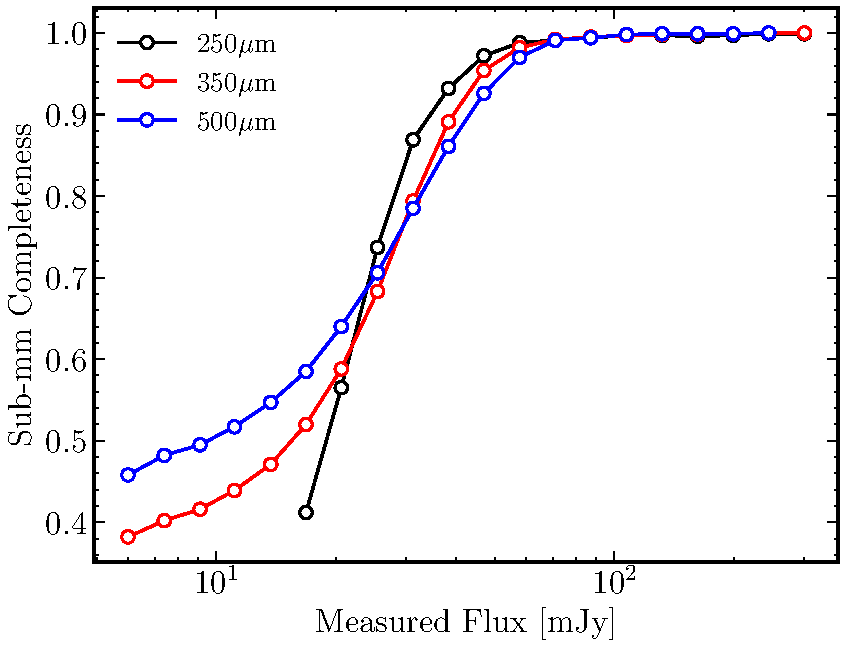
\includegraphics[width=\columnwidth]{Figures/submm_completeness.pdf}
	\caption{The completeness of the H-ATLAS Data Release I catalogues of sub-mm sources, as a function of the measured flux density at 250\,\micron (black) 350\,\micron (red) and 500\,\micron (blue). This figure is replotted from Figure 21 in \citealt{Valiante_2016}.}
	\label{fig:submm_completeness}
\end{figure}

\subsection{Data Releases of the H-ATLAS}
\label{sec:Data Releases of the H-ATLAS}

The first public data release (DR1) of H-ATLAS covered the three equatorial GAMA fields, which span approximately 25\% of the total survey area. These fields benefit from multiwavelength coverage from GAMA, SDSS, 2dF, the Galaxy Evolution Explorer (GALEX, \citealt{Martin_2005}), the UKIRT Infrared Deep Sky Survey -- Large Area Survey (UKIDSS-LAS, \citealt{Lawrence_2007}), the Wide-field Infrared Survery Explorer (WISE, \citealt{Wright_2010}), the VISTA Kilo-degree Infrared Galaxy survey (VIKING, \citealt{Edge_2013}) and the Kilo-Degree Survey (KiDS, \citealt{deJong_2013}). 

Sources are provided with DR1 if they are detected above the 2.5$\sigma$ detection limit on the 250\,\micron map and have measured flux densities greater than the 4$\sigma$ flux density limits in one of the three SPIRE bands (29.6\,mJy, 37.6\,mJy or 40.8mJy at 250, 350 and 500\,\micron). Across the three fields there are a total of 113,995, 46,209 and 11,011 sources detected at > 4$\sigma$ at 250, 350 and 500\,\micron as well as detections for 4,650 and 5,685 sources at > 3$\sigma$ at 100 and 160\,\micron (\citealt{Valiante_2016}). Following the release of the sub-mm sources detected in the GAMA fields, \citealt{Bourne_2016} used the Likelihood Ratio (LR, \citealt{Sutherland_1992}; \citealt{Ciliegi_2003}) method (Section \ref{sec:The Likelihood Ratio Method}) to identify potential optical counterparts to the 113,995 sources with SNR$_{250}$ > 4 from SDSS. Sources with SNR$_{250}$ < 4 that were detected by their 350 or 500\,\micron flux densities were omitted from the matching since these sources have sub-mm colours suggesting a high redshift, and are the most likely sources to be misidentified by SDSS due to the increased probability of chance alignments or gravitational lensing along the line of sight (\citealt{Negrello_2010}; \citealt{Pearson_2013}; \citealt{Bourne_2014}). \citealt{Bourne_2016} found optical counterparts within 10" of 44,385 (39\%) sources with an estimated probability of being the true ID > 80\% (the probability of an optical or near-infrared object being the true counterpart to a sub-mm source is defined as the reliability, R, and is derived in Section \ref{sec:The Likelihood Ratio Method}).

The second public data release (DR2) covered the NGP and SGP, two large fields that together form $\sim$\,75\% of the total survey area. The NGP was covered in the optical by the SDSS and in the near-infrared by UKIDSS-LAS. Moreover, a small area of 25.93\,$\deg^2$ within the NGP was also observed by a deeper K-band survey by the H-ATLAS team using UKIRT (limiting magnitude of K < 19.40 compared to K < 18.69 for UKIDSS-LAS). The SGP is the largest field (approximately half the survey area of H-ATLAS) and was covered by the 2dF spectroscopic survey, KiDS in four optical bands ($u$, $g$, $r$ and $i$) and VIKING in five near-infrared bands ($Z$, $Y$, $J$, $H$ and $K_s$).

Given that sub-mm sources are only extracted from areas of the \textit{Herschel} maps that have at least two obsersations from the SPIRE instrument, the DR2 catalogues includes sources from the map area reduced by the masking of single \textit{Herschel} scans. The mask reduces the area covered by the NGP point source catalogue to 177.1\,$\deg^2$ and the SGP to 303.4\,$\deg^2$. As with DR1, sources are included if they are detected on the 250\,\micron map above the 2.5$\sigma$ detection limit by the MADX algorithm and surpass at least one of the 4$\sigma$ flux density limits at the SPIRE wavelengths. The catalogues contain 118,980 sources for the NGP field (112,069, 48,876 and 10,368 detected at > 4$\sigma$ at 250, 350 and 500\,\micron and 5,036 and 7,046 at > 3$\sigma$ at 100 and 160\,\micron respectively) and 193,527 sources for the SGP field (182,282, 74,096 and 16,084 at 250, 350 and 500\,\micron and 8,598 and 11,894 at 100 and 160\,\micron). \citealt{Furlanetto_2018} applied the Likelihood Ratio method to all counterparts within 10" of the 250\,\micron sources of the NGP using both the shallower optical and near-infrared catalogue of SDSS and UKIDSS-LAS, and the deeper K-band survey. Of the 112,155 SPIRE sources with SNR$_{250}$ > 4, 77,521 (69.1\%) had at least one shallow optical counterpart and 42,429 (37.8\%) of these were matched with R > 0.8. In the smaller area observed with WFCAM, \citealt{Furlanetto_2018} identified 32,041 possible deep near-IR counterparts to 17,247 sources. 10,668 (61.9\%) of these sources were matched with an equally high reliability. While this analysis suggests that the inclusion of deeper K-band data drastically increases the fraction of sources matched to their corresponding optical or near-IR counterpart, [...]\todo[color=yellow]{continuation: we must consider their differences and think about Q}.

In the SGP a preliminary counterpart analysis was conducted using the Two Micron All Sky Survey (2MASS, \citealt{Skrutskie_2006}), but no formal LR analysis had yet been applied. A nearest neighbour match within 5" of a 2MASS galaxy gives identifications for 3,444 \textit{Herschel} sources. In the following section we detail the Likelihood Ratio method and apply it to the 250\,\micron sources detected by \textit{Herschel} in the SGP.

\subsection{Identifying Optical and Near-IR Counterparts to Herschel Sources}
\label{sec:Identifying Optical and Near-IR Counterparts to Herschel Sources}

When identifying multiwavelength counterparts across surveys the simplest choice to use the nearest neighbour within a fixed search radius of one of the sources. For surveys conducted at similar wavelengths with a similar resolution and sensitivity this is a suitable approach. However, when matching far-IR/sub-mm surveys to optical/IR data, the poor angular resolution of long wavelength instruments such as SPIRE (the FWHM of 250\,\micron detections with SPIRE is $\sim$ 18"), which cause large positional uncertainties, force us to increase the search radius around the sub-mm source. This effect, coupled with the intrinsic faintness of optical/near-IR counterparts due to dust obscuration, the relatively flat redshift distribution of sub-mm sources due to the k-correction and the high surface density of objects in optical/IR surveys, means that [...]\todo[color=yellow]{continuation: identification is not easy, Casey reference?} and it is common for there to be multiple possible counterparts within the search radius from a single sub-mm source.

Previously for sub-mm surveys it would be more practical to first match sources with radio or mid-IR sources and then use pre-existing matched catalogues to obtain multiwavelength data (e.g. \citealt{Ivison_2007}; \citealt{Dye_2009}; \citealt{Biggs_2011}, see also Section [...]\todo[color=green]{add reference for the final chapter}). However, presently this is not suitable for large surveys such as H-ATLAS as current radio telescopes do not provide the area and depth required to match with more than a small fraction of sub-mm sources. While current and future radio surveys from facilities such as the Square Kilometre Array (SKA), the Low Frequency Array (LOFAR) and MeerKAT will increase the radio coverage of the H-ATLAS fields, currently a statitstical identification method is still the preferred way of deciding which objects are associated and which are unrelated foreground/background objects to large samples of sub-mm sources.

\subsection{The Likelihood Ratio Method}
\label{sec:The Likelihood Ratio Method}

The Likelihood Ratio method assigns a probability (reliability) to all potential matches surrounding low resolution sources to distinguish between likely counterparts and chance alignments and has been used many times to identify counterparts to \textit{Herschel} sources. The LR method was used by \citealt{Smith_2011} to identify SDSS counterparts in the Science Demonstration Phase (SDP) catalogue (a preliminary data release for H-ATLAS, overlapping with the GAMA9 field), by \citealt{Kim_2012} to identify Spitzer-IRAC counterparts also in the SDP data, by \citealt{Fleuren_2012} for VIKING IDs in the Phase 1 catalogue of the GAMA9 field, and as mentioned earlier, by \citealt{Bourne_2016} and \citealt{Furlanetto_2018} to find optical and near-IR counterparts in the GAMA fields and NGP field respectively.

The likelihood, $L$, of a counterpart being the true identification to a \textit{Herschel} source is given by the ratio between the probability that an object observed at a given radius from the source, $r$, with an optical or near-IR magnitude, $m$, is the true identifcation and the probability of observing an unassociated object with the same $r$ and $m$. On the assumption that the distance from the source and the optical/near-IR magnitude are independent on their influence on the probability of being a true counterpart, we find that:

\begin{equation}
\label{eq:likelihood_ratio}
    L = \frac{P(\textrm{ID}, r, m)}{P(\textrm{unassociated}, r, m)} = \frac{P(\textrm{ID}, r) P(\textrm{ID}, m)}{P(\textrm{unassociated}, r, m)}
\end{equation}

Each term in the above equation can be defined in the following way: $f(r) \coloneqq P(\textrm{ID}, r)$, $q(m) \coloneqq P(\textrm{ID}, m)$ and $n(m) \coloneqq P(\textrm{unassociated}, r, m)$, where $f(r)$ represent the radial probability distribution function of positional errors between the source and counterpart, $q(m)$ represents the magnitude probability distribution of true counterparts and $n(m)$ is the magnitude distribution of background objects from the input survey. By using Baye's theorem and the theorem of total probability, we can define the probability that a counterpart is the true ID given it has $r$ and $m$ as:

\begin{equation}
\label{eq:reliability_one_counterpart}
    R \coloneqq P(\textrm{ID}| r, m) = \frac{L}{L+1}.
\end{equation}
\todo[color=green]{Requires a derivation}

Equation \ref{eq:reliability_one_counterpart} assumes that there is only a single candidate with a likelihood $L$. For a source with multiple possible candidates, the reliability $R_j$ of the $j^{th}$ candidate is given by:

\begin{equation}
    \label{eq:reliability_multiple_counterparts}
        R_j = \frac{L_j}{\sum_i L_i + (1-Q)},
\end{equation}

where $i$ represents the $i^{th}$ counterpart found within the search radius. The $Q$ parameter represents the fraction of all true counterparts that are brighter than the limiting magnitude of the input survey and can therefore be observed. This means that the (1 - $Q$) term represents the probability that the counterpart is not observed and accounts for the fact that not all counterparts will be detected in the optical/near-IR survey. The value of $Q$ depends on the depth of the survey and the choice of passband used. In the following sections I shall outline the methods used to estimate the functions $f(r)$, $q(m)$ and $n(m)$ and to estimate $Q$ to calculate the likelihood ratios and reliabilities of near-IR counterparts observed on the VIKING images surrounding the 250\,\micron positions of \textit{Herschel} sources in the SGP.

\section{Applying the LR Method to VIKING Galaxies in the SGP}
\subsection{VISTA VIKING Counterparts}

The Visible and Infrared Survey Telescope for Astronomy (VISTA) is a 4\,m wide field telescope located at the ESO Paranal Observatory in Chile. The telescope has five near-IR broad band filters, $Z$, $Y$, $J$, $H$ and $K_s$, that have central wavelengths between 0.88 and 2.15\,\micron (\citealt{Emerson_2010}). The VIKING survey was a public survey with VISTA, covering approximately 1,500\,$\deg^{2}$ of sky, including an overlap of more than 360\,$\deg^{2}$ with the H-ATLAS survey in the GAMA and SGP fields, to a 5\,$\sigma$ depth of 23.1, 22.3, 22.1, 21.5 and 21.2 (AB) in the above five filters.

We take as our object catalogue all objects observed in the fourth data release of VIKING within 15" of the 250\,\micron position of each \textit{Herschel} source. The counterpart matching in the GAMA9 field by \citealt{Fleuren_2012}, recovered 51\% of all 250\,\micron sources with a reliable (R > 0.8) VIKING counterpart. Compared to the optical r-band of the SDSS as used in \citealt{Bourne_2016} and \citealt{Furlanetto_2018} which have typical returns of $\sim$ 35 -- 40\% due to the limiting magnitude of SDSS, we expect the SGP to have reliable identifications for approximately half of all SGP sources. The SGP fields contains 193,527 sources detected at greater than 4\,$\sigma$ significance, suggesting that we might expect to match $\sim$ 100,000 \textit{Herschel} sources with a near-IR counterpart with a high probability.

However, a significant number of sources in the VIKING survey are stars that would be erroneously matched to H-ATLAS. The sub-mm emission from stars is most likely from debris discs or dust in outflows. As there is large variation in the mass and temperature of debris discs for stars of a given spectral type (\citealt{Hillenbrand_2008}), and \textit{Herschel} is only sensitive to the brightest of these discs (\citealt{Thompson_2010}), there is much scatter in the sub-mm properties of \textit{Herschel} detected stars which would result in poor statistics of dusty stars when calculating the likelihood of counterparts. For this reason, I use an adapted method of \citealt{Baldry_2010} to separate stars and galaxies in the VIKING SGP catalogue and apply the LR method separately for the two classes.

The method of \citealt{Baldry_2010} uses near-IR $J$ and $K_s$ and optical $g$ and $i$ bands to define a line of separation between stars and galaxies in $J - K_s$, $g-i$ colour-colour space, and is used in \citealt{Bourne_2016} and \citealt{Furlanetto_2018} to separate stellar and extragalactic objects in SDSS. Without coverage from SDSS in the SGP, I use the fourth data release of KiDS to identify optical $g$ and $i$ bands for [...]\todo[color=green]{Look up value} of our VIKING sources. A nearest neighbour search to a maximimum of 0.5" from the 250\,\micron position of each source was used.

First, I classify as stellar any object in our catalogue with \texttt{pStar} > 0.95, an estimate of the probability that the source is a star, based on a shape parameter provided as part of the VIKING data release. This immediately classifies 51,508 objects as stars. Next I consider the $J - K_s$, $g-i$ colour-colour space and define a stellar locus by converting the locus in \citealt{Baldry_2010} to the Vega system assuming $J_{\textrm{Vega}}$ = $J_{\textrm{AB}}$ - 0.91 and $K_{s,\textrm{Vega}}$ = $K_{s,\textrm{AB}}$ - 1.85:

\begin{equation}
    f_{\textrm{locus}} = 
    \begin{cases*}
        0.228 & $g-i$ < 0.3 \\
        0.05 + 0.615(g-i) - 0.13(g-i)^2 & 0.3 $\leq$ $g-i$ < 2.3 \\
        0.7768 & $g-i$ $\geq$ 2.3.
    \end{cases*}
\label{eq:stellar_locus}
\end{equation}

I define a line of separation between stars and galaxies as being +0.2 offset in $J - K_s$ from the stellar locus. The distribution of sources, stellar locus and separation line are illustrated in Figure \ref{fig:star_galaxy_classification}. This classifies a further 411,463 sources that have KiDS identifications (299,525 extragalactic and 111,938 stellar). The remaining objects do not have matches in KiDS and thus do not have $g$ and $i$-band magnitudes. However, based on the separation line defined above, it can be seen that those objects with $J - K_s$ < 0.42 will always fall below the separation line regardless of their optical colour, and similarly, any object with  $J - K_s$ > 0.98 will always lie above the line. The cross contamination of stars above the line and galaxies below the line is small, so I next define all remaining sources using the above single flux cuts. This classifies a further 102,540 sources (102,265 as galaxies and 275 as stars). Finally, I return to the \texttt{pStar} parameter and relax the criteria to those objects with \texttt{pStar} > 0.7; all other objects are classified as galaxies. This method leads to the identifcation of 793,331 (78.9\%) extragalactic sources and 212,028 (21.1\%) stars.

\begin{figure}
	\includegraphics[width=\columnwidth]{Figures/star_galaxy_classification.pdf}
	\caption{The $J - K_s$, $g-i$ colour-colour diagram of VIKING objects with KiDS identifications in the SGP. The stellar locus defined by Equation \ref{eq:stellar_locus} is illustrated as the blue line, while the separation between stars and galaxies, defined as +0.2 offset from the stellar locus, is shown as a dashed blue line. Extragalactic and stellar sources identified from our classification are shown as grey and red points respectively.}
	\label{fig:star_galaxy_classification}
\end{figure}

\subsection{Distribution of True Counterparts, q(m)}
\label{sec:true_counterparts_distribution}

To estimate the reliability of each VIKING source being the true ID to a \textit{Herschel} source, I determine the probability distribution of true counterparts as a function of $K_s$-band magnitude, $q(m)$, using the method described in \citealt{Ciliegi_2003}. First, a magnitude distribution of all objects found in the VIKING images within 15" of a \textit{Herschel} source is generated separately for stars and galaxies, which we shall denote as $n'_{\textrm{total}}(m)$. Here I have set prime notation to reference raw counts, while no prime notation is reserved for counts that have been normalized by the total area searched on the VIKING images. The excess of sources above the background level in regions surrounding the 250\,\micron sources is an estimate for the number density of true VIKING associations and is estimated by subtracting the magnitude distribution for the whole VIKING survey from $n'_{\textrm{total}}(m)$. A set of 844,715 random positions were located on the SGP map and used to search for objects on the VIKING images to within 15". A total of 2,917,214 objects were found and form our $n'_{\textrm{background}}(m)$ distribution. The excess of "real" counterparts thus has a magnitude distribution that may be expected to follow

\begin{equation}
    n'_{\textrm{real}}(m) = n'_{\textrm{total}}(m) - n'_{\textrm{background}}(m) \frac{N_{\textrm{250\,\micron}}}{N_{\textrm{background}}},
\end{equation}

where the distribution has been scaled to the search area by $N_{\textrm{250\,\micron}}$ and $N_{\textrm{background}}$, the number of 250\,\micron positions and the number of randomly located positions respectively.

I then derive the $q(m)$ distribution by normalizing $n_{\textrm{real}}(m)$ and scaling by the fraction of all true counterparts that would be visible on the VIKING images, $Q$. This ensures that the integral of $q(m)$ over all magnitudes up to the limiting magnitude of the VIKING survey is equal to the probability that the sources is detected, i.e. $\int^{m_{\textrm{lim}}} q(m)dm = Q$. This normalization can be written as:

\begin{equation}
\label{eq:true_counterparts_distribution}
    q(m) = \frac{n'_{\textrm{real}}(m)}{\sum_{m_i}n'_{\textrm{real}}(m_i)}\times Q,
\end{equation}

where we have summed over the magnitude bins, $m_i$. The magnitude distribution of "true" counterparts to the 250\,\micron SGP sources is illustrated in the middle panel of Figure \ref{fig:true_counterparts_distribution} and shows the difference between the two distributions for extragalactic and stellar sources, requiring us to implement the LR method separately for the two classes. I also show in Figure \ref{fig:true_counterparts_distribution} the magnitude distributions of $n_{\textrm{total}}$ and $n_{\textrm{background}}$ and the distributions $q(m)/n(m)$ (here $n(m)$ references the area-normalized background distribution of sources, as used in Equation \ref{eq:likelihood_ratio} to calculate the likelihood values). The calculation of the likelihood value for each VIKING source thus depends on an estimate for the fraction of true IDs that are observed on the VIKING images, $Q$, which I detail in the following section.

\begin{figure}
    \centering
	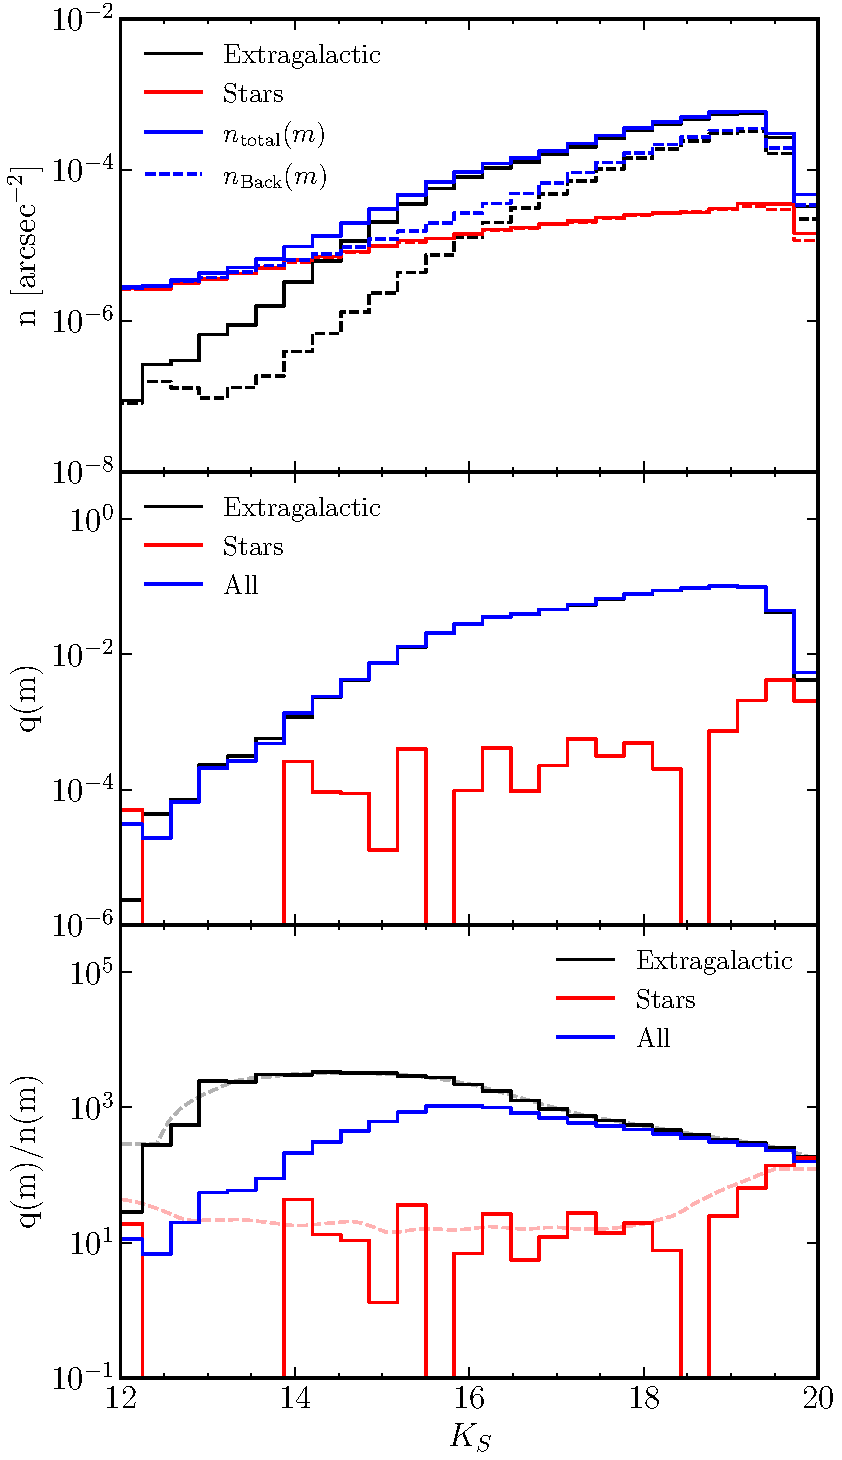
\includegraphics[height=0.75\textheight]{Figures/true_counterparts_distribution.pdf}
	\caption{Top panel: The $K_s$-band magnitude distributions of objects located within 15" of 250\,\micron \textit{Herschel} positions (blue solid line) and random positions (blue dashed line), also separated by extragalactic (black lines) and stellar (red lines) identifications. Middle panel: The $K_s$-band magnitude distribution of "true" counterparts accounting for the excess of VIKING sources observed near \textit{Herschel} sources. Bottom panel: The ratio between the "true" counterparts distribution (middle panel) and the background distribution of sources, as used in the calculation of likelihoods; Equation \ref{eq:likelihood_ratio}. The dashed lines represent smoothed fits to $q(m)/n(m)$ to provide a continuous function at all magnitudes. The colour convention of the middle and bottom panels are the same as the top panel.}
	\label{fig:true_counterparts_distribution}
\end{figure}

\subsection{Estimating Q}

I predict the probability of finding a genuine counterpart in the VIKING images above the limiting magnitude using the method described in \citealt{Fleuren_2012}. While some methods estimate $Q$ directly by totaling the $n_{\textrm{real}}(m)$ distribution and dividing by the number of SPIRE sources, this leads to a systematic overestimate due to the possibility of clustering of galaxies or multiple counterparts to the sub-mm source due to source blending. An alternative method by \citealt{Fleuren_2012} calculates an estimate of 1-$Q_0$, the probability of not observing a VIKING counterpart, by counting the number of sub-mm sources without VIKING associations within a search radius, $r$. These sources will be given the name \textit{blanks}, and has a dependency on search radius, $B(r)$.

Blank sources may be observed in one of several scenarios. The most likely reason (given the limiting depth of VIKING compared to \textit{Herschel}, see Figure [...]\todo[color=orange]{If I include a plot that compares the depth of the surveys against Herschel limits, add reference here.}) is that the real source is fainter than the VIKING $K_s$-band limit. However, a blank may also be observed if the counterpart lies outside the search radius or if the sub-mm source is a spurious SPIRE detection.

While we may observe a sub-mm source with a possible VIKING candidate, we may not definitively say that a source is not a blank as we may encounter chance alignments with VIKING sources close to the same line of sight. Thus, to estimate the true number of blanks, we are reminded that the number of blanks we observe must also account for those that are spuriously identified as not blank. In other words, the number of observed blanks is the number of true blanks minus the number of true blanks that have random VIKING interlopers. If we define the number of observed blanks as $B_{\textrm{obs}}$, the number of true blanks as $B_{\textrm{t}}$ and the number of random interlopers as $N_{\textrm{rand}}$, then

\begin{equation}
    B_{\textrm{obs}} = B_{\textrm{t}} - N_{\textrm{rand}} = B_{\textrm{t}} - B_{\textrm{t}} \times f_{\textrm{rand}},
\end{equation}

where we have assumed that the number of random interlopers can be estimated from the fraction of positions that have random interlopers, $f_{\textrm{rand}}$. This fraction can be estimated from the set of random positions used above to calculate $q(m)$. Using a similar set of notation: $B_{\textrm{background}}$ to represent the number of blank positions from the catalogue of random positions; $N_{\textrm{background}}$ to represent the number of random positions; and $B'_{\textrm{background}}$ representing the number of random positions for which a VIKING counterpart was observed (or non-blank), we can estimate $f_{\textrm{rand}}$ as:

\begin{equation}
    f_{\textrm{rand}} = \frac{B'_{\textrm{background}}}{N_{\textrm{background}}} = \frac{N_{\textrm{background}} - B_{\textrm{background}}}{N_{\textrm{background}}} = 1 - \frac{B_{\textrm{background}}}{N_{\textrm{background}}}.
\end{equation}

To scale this fraction to the size of the SPIRE catalogue, the same number of random positions are used as there are 250\,\micron positions, such that $f_{\textrm{rand}}$ may be written as:

\begin{equation}
    f_{\textrm{rand}} = 1 - \frac{B_{\textrm{background}}}{N_{\textrm{250\,\micron}}}.
\end{equation}

From substitution we find that the fraction of \textit{Herschel} sources that are true blanks (i.e. $B_{\textrm{t}}/N_{\textrm{250\,\micron}}$), is given by:

\begin{equation}
    \frac{B_{\textrm{t}}}{N_{\textrm{250\,\micron}}} = \frac{B_{\textrm{obs}}}{B_{\textrm{background}}}.
\end{equation}

In summary, to estimate 1-$Q$, we need only to divide the number of observed blank 250\,\micron positions by the number of observed blank random positions. It is clear that any estimate of $Q$ using this method depends on the given search radius from the sub-mm source, $r$, thus I calculate this fraction for a range of radii between 0" and 15" and model the dependence of $B(r) \coloneqq 1 - Q$ on the search radius in the same manner as \citealt{Fleuren_2012}. 

A sub-mm source that has no true VIKING association within a radius $r$ is either a source whose counterpart is too faint to be detected by the VIKING survey or lies outside the radius, or both. Assuming that such situations are independent of each other (i.e. a true VIKING candidate that lies at higher offsets from the sub-mm source than average is not also fainter and vice versa), then the probability of either occurring is given by the conditional probability:

\begin{equation}
    P(\textrm{Blank}) = P(\textrm{Faint} \cup \textrm{Outside}) = P(\textrm{Faint}) + P(\textrm{Outside}) - P(\textrm{Faint} \cap \textrm{Outside}).
\end{equation}

The first term, the probability that the counterpart is too faint to be detected is given by 1-$Q$, while the probability that the counterpart resides outside the search radius is dependent on the distribution of offsets between the counterpart and sub-mm source, $f(r)$. This distribution represents the probability that a real counterpart is found at a radial distance $r$ from the SPIRE source, where we assume that the H-ATLAS sources are point-like on the 250\,\micron maps and that the errors are equal in RA and declination for radial symmetry.

While $f(r)$ depends on both the positional errors of the sub-mm and the VIKING catalogues, we can assume that the near-IR positional errors are negligible compared to those of SPIRE given that the 1$\sigma$ VIKING positional errors are < 0.2" (\citealt{Fleuren_2012}), while the FWHM of the 250\,\micron beam used to extract the \textit{Herschel} sources is $\sim$ 18". As such, I use a radially symmetric Gaussian with width $\sigma_\textrm{pos}$ as $f(r)$. Accordingly with the theory of total probability, the probability that an observable counterpart is detected out to any search radius must equal unity, thus our function $f(r)$ is normalized such that:

\begin{equation}
    \int_0^\infty 2\pi f(r')r'dr' = 1,
\end{equation}

which implies for our Gaussian distribution that

\begin{equation}
    f(r) = \frac{1}{2\pi\sigma_\textrm{pos}^2}e^{\frac{-r^2}{2\sigma_\textrm{pos}^2}}.
\label{eq:positional_offset_distribution}
\end{equation}
[...]\todo[color=orange]{Requires a derivation.}

Returning to the probability that a VIKING counterpart is not observed within a radius $r$, we can estimate this as 1 - $F(r)$ where $F(r)$ relates to $f(r)$ as

\begin{equation}
    F(r) = \int_0^r 2\pi r'f(r')dr'.
\end{equation}

Upon substitution we thus find that the probability of observing a blank source as a function of the search radius can be modelled as

\begin{equation}
    B(r) = P(\textrm{Blank}) = (1-Q) + (1-F(r)) - (1-Q)(1-F(r)) = 1 - QF(r)
\label{eq:blanks_model}
\end{equation}

In Figure \ref{fig:Q_estimate} I show the observed number of blank \textit{Herschel} (open squares) and random (open circles) positions as a function of the search radius, as well as their ratio which is our estimate of $B_{\textrm{t}}/N_{\textrm{250\,\micron}}$ (filled circles). The best fitting $B(r)$ is illustrated as the black line. Using this method I estimate the value of $Q$ to be $0.835\pm0.009$ when considering all VIKING objects and $Q=0.823\pm0.009$ when stellar contaminants are removed.

\begin{figure}
    \centering
	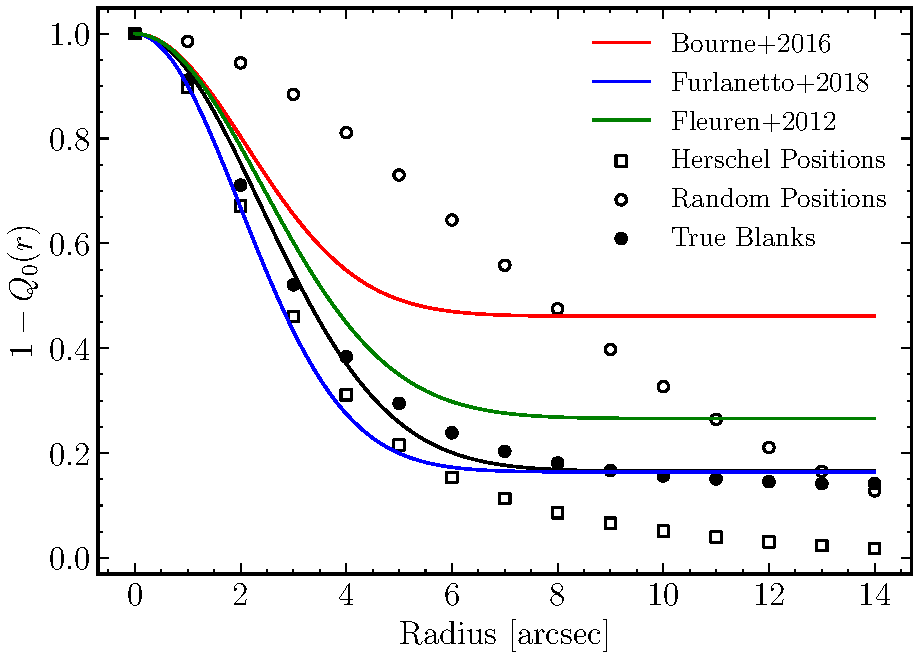
\includegraphics[width=\columnwidth]{Figures/Q_estimate.pdf}
	\caption{Estimates for the number of blanks (sources without VIKING candidates) as a function of the search radius, $r$. Open circles represent the number of blank random positions placed across the SGP, while open squares represent the number of blank SPIRE 250\,\micron positions from H-ATLAS. The filled circles shows the division of the former by the latter, representing our estimate for the true fraction of SPIRE sources that are blank on the VIKING images. The solid black line represents the best fit to the points using Equation \ref{eq:blanks_model}. The same model used in \citealt{Fleuren_2012}, \citealt{Bourne_2016} and \citealt{Furlanetto_2018} are shown as green, red and blue lines respectively.}
	\label{fig:Q_estimate}
\end{figure}

Previous estimates of $Q$ from r-band SDSS candidates in the other H-ATLAS fields have taken lower values as a result of the difference in depth between SDSS and VIKING. In DR1 \citealt{Bourne_2016} measured the value of $Q$ for all SDSS objects observed in the GAMA fields to be $0.539\pm0.001$, and \citealt{Furlanetto_2018} measured a near identical value of $Q=0.538\pm0.001$ in the NGP during DR2. However, my value of $Q$ is similar to that found by \citealt{Fleuren_2012}, $Q = 0.7342\pm0.0257$ and is almost identical to the value of $0.836\pm0.001$ found from the deep K-band analysis by \citealt{Furlanetto_2018}. As a collection, these estimates indicate that a survey of VIKING candidates returns a greater probability of observing a galaxy near a sub-mm source than an SDSS survey due to the increase in depth. A comparison between data releases due to the available input survey is made in Section [...]\todo[color=orange]{If a comparison between data releases is made, add the section reference here.} and in Table \ref{tab:data_release_input_surveys} I detail the various estimates made for $Q$ during analyses of H-ATLAS sources alongside their input surveys, passbands used and their depths.

\begin{table}
\centering
\begin{tabular}{|p{6.5cm}|p{3.5cm}|p{2.5cm}|p{4cm}|}
    \hline
    H-ATLAS & Input Survey & $Q$ Estimate & Reference \\
    \hline
    \hline
    Science Demonstration Phase (SDP) & SDSS -- ($r < 22.4$) & $0.583$ & \citealt{Smith_2011} \\ 
    Phase 1 GAMA9 & VIKING -- ($K_s < ??$) & $0.734\pm0.026$ & \citealt{Fleuren_2012} \\
    Data Release I & SDSS -- ($r < ??$) & $0.539\pm0.001$ & \citealt{Bourne_2016} \\
    Data Release II & SDSS -- ($r < ??$) & $0.538\pm0.001$ & \citealt{Furlanetto_2018} \\
    Data Release II & UKIRT -- ($K_s < ??$) & $0.836\pm0.001$ & \citealt{Furlanetto_2018} \\
    Data Release III & VIKING -- ($K_s < ??$) & $0.835\pm0.009$ & This work \\
    \hline
\end{tabular}
\caption{Comparison of the input survey passbands, depths and measured values of $Q$. From left to right the columns contain: i) the corresponding data release of H-ATLAS, ii) the input survey, passband used and its limiting magnitude, iii) the fraction of true sources observed on the survey images, $Q$, iv) reference.}
\label{tab:data_release_input_surveys}
\end{table}
\todo[color=orange]{Complete Table.}

\subsection{Positional Uncertainty of H-ATLAS Detections}

The fitting function of Equation \ref{eq:blanks_model} also provides an estimate for the standard positional error, $\sigma_{\textrm{pos}}$ which defines the width of the positional offset distribution $f(r)$. I measure this value to be $\sigma_{\textrm{pos}} = 2.388\pm0.065"$, representing the average error in the 250\,\micron positions. We see in Figure \ref{fig:Q_estimate} that $B(r)$ becomes flat at approximately 3$\sigma_{\textrm{pos}}$, suggesting that few counterparts are to be found at search radii greater than $\sim$ 7". It also interesting to note that the model underpredicts the number of blank sources between 4 $\lesssim$ r $\lesssim$ 8 arcsec, but overpredicts at the highest search radii. This has been observed previously (e.g. \citealt{Fleuren_2012}) and might suggest clustering of VIKING objects which is not modelled in $B(r)$.

The positional uncertainty has a dependency on the SNR of the sub-mm detection (\citealt{Bourne_2016}) and in theory should depend on the ratio between the FWHM of the observations and the SNR as given by

\begin{equation}
    \sigma_{\textrm{pos}} = 0.6\times\frac{\textrm{FWHM}}{\textrm{SNR}},
\label{eq:positional_uncertainty_theory}
\end{equation}

as detailed by \citealt{Ivison_2007} on the assumption of uncorrelated noise. However, the prefactor is likely to be increased by confusion noise in the maps and clustering (\citealt{Chapin_2011}; \citealt{Bourne_2014}) and so a scaling factor (typically about 1.09, corresponding to a redefined prefactor of $\sim$ 0.65) is applied and is more suitable for sources detected on sub-mm images. To define an individual value of the 1$\sigma$ positional uncertainty, and thus a separate $f(r)$ for each detection, I implement an empirical version of Equation \ref{eq:positional_uncertainty_theory} of the form

\begin{equation}
    \sigma_{\textrm{pos}} = k\times\frac{\textrm{FWHM}}{\textrm{SNR}},
\label{eq:positional_unceratinty_empirical}
\end{equation}

where $k$ is a constant to be determined. Using FWHM = 18", the fitted value of $\sigma_{\textrm{pos}} = 2.388$ and  the SNR of each 250\,\micron detection, I generate a set of $k$ values. I take the median value of the distribution of $k = 0.66$ as my constant. This value is used in Equation \ref{eq:positional_unceratinty_empirical} to determine $f(r)$ for each object's likelihood calculation.

A more refined method of determining $\sigma_{\textrm{pos}}$ is outlined in \citealt{Smith_2011} and applied in other works (e.g. \citealt{Bourne_2014}, \citealt{Bourne_2016} and \citealt{Furlanetto_2018}), though is also an empirical measurement. In such studies, a 2D histogram is derived for the offsets between sub-mm sources and optical/near-IR objects within a large box around each SPIRE source (typically 50" or more). This histogram can be modelled in shape by three contributing populations: i) a random background of chance alignments which should be observed as a constant since the probability of a chance alignment is equal along any line of sight; ii) the population of true IDs whose positional offset distribution follows $f(r)$ for a fraction $Q$ of all sources and iii) nearby counterparts that are physically correlated with the sub-mm source due to galaxy clustering but are not the true IDs, which requires an understanding of the cross-correlation between the sub-mm and optical/near-IR samples. Further details on the modelling of these histograms can be found in \citealt{Smith_2011}. By binning the sub-mm sources by their SNR and fitting the 2D histograms with a model considering the above contributions, an estimate can be made for $\sigma_{\textrm{pos}}$ as a function of SNR. Assuming a powerlaw dependence of the form $\sigma_{\textrm{pos}} = \sigma_{\textrm{pos}}(5) [\textrm{SNR}/5]^\alpha$ where $\sigma_{\textrm{pos}}(5)$ is the positional uncertainty of a 250\,\micron detection with SNR = 5, and by binning the sources further by sub-mm colour, it has been shown that the bluest SPIRE sources ($S_{250}/S_{350}$ > 2.4) have a dependence of $\sigma_{\textrm{pos}}$ on SNR that is not significantly different from the theoretical model given in Equation \ref{eq:positional_uncertainty_theory} (\citealt{Bourne_2016}; \citealt{Furlanetto_2018}). As shown in these studies the powerlaw function shifts to higher values of $\sigma_{\textrm{pos}}$ as we tend to redder sources. A possible explanation for a broader distribution of offsets for redder SPIRE sources is due to an increased probability of these sources being at higher redshifts and thus an increased contribution of foreground structures lensing the source. To avoid this bias, $\sigma_{\textrm{pos}}$ could be measured from the 2D histogram of positional offsets of the bluest sources, but for a model dependence that is reasonable for the majority of sources, a multiplicative factor should be included, leading to the prefactor of $k$ commonly assumed being larger than 0.6. Given that the simple method used here provides a similar value of $k$, I do not expect there to be any systematic differences in the likelihood calculations for SGP sources and the aforementioned papers as a result of the different methods used to calculate $\sigma_{\textrm{pos}}$.

\section{Likelihood Ratio Results}

I apply the likelihood ratio to all possible VIKING counterparts within 15" of a SPIRE source. The catalogue contains 193,527 sub-mm sources, of which 190,788 have at least one possible counterpart identified within the search radius. Within this sample, 180,030 are sources with SNR$_{250}$ > 4. Having identified each source with its highest reliability counterpart I find that 181,373 (95.1\%) are sources with VIKING identifications indicating the source is a galaxy and 9,415 (4.9\%) with stellar classifications. 

In keeping with previous studies I define reliable matches as those sources with counterparts having $R \geq 0.8$ in order to minimize the number of false counterparts while maintaining a sample that is dominated by sources with a low chance of blending and thus the FIR emission is likely dominated by a single source. I identified 111,065 reliable near-IR counterparts, representing 58.2\% of all sources with at least one possible candidate. Of the reliable IDs, 110,374 (99.4\%) are classified as extragalactic and 691 (0.6\%) as stellar. The increase in the fraction of galaxies and reduction in stars compared to the input VIKING survey suggests that the LR method is highly biased against stars as is intended.

On the assumption that a source that is erroneously matched with a counterpart has a probability of $1 - R$, we can estimate the false ID rate for our reliable matches:

\begin{equation}
    N_{\textrm{False}} = \sum_{R_i \geq 0.8} (1 - R_i) = 5,343.
\label{eq:false_ids}
\end{equation}

I predict that there are 5,343 "false reliable" IDs in the SGP, representing 4.8\% of the reliable sample. This can be compared to values of 4.7\% in the GAMA fields and the NGP (optical SDSS matching), 4.5\% for the NGP (near-IR deep matching) and 4.2\% during the SDP. While the value for the SGP is in keeping with the other H-ATLAS fields, it is the highest false identification rate. It would be expected that the near-IR analyses would have the lowest false identification rates as the optical r-band restricts the limiting redshift of the counterparts to lower redshifts than the near-IR K-band (see Figure [...]\todo[color=orange]{If a figure showing the different redshift depths of surveys is made, add reference here}). As a result, the contamination of high redshift sub-mm sources that are falsely identified with low redshift optical counterparts is expected to be higher, increasing the false identification rate. However, in the analysis of the SGP, we choose to use an increased search radius of 15" (compared to 10" as used in previous H-ATLAS studies) which increases the average number of counterparts found per source. Given the requirement of the LR method that the sum of the reliabilities of all possible candidates to a source must not exceed one, the increased average number of candidates reduces the average reliability of the true ID and thus increases the false identification rate - likely by a factor greater than the reduction caused by using the near-IR VIKING survey compared to SDSS. Further discussion on the effect of increasing the search radius is made in Section X [...]\todo[color=green]{Add reference to multiplicity section}. The initial choice to use a search radius of 15" came from recent studies suggesting that genuine associations are found on the VIKING images beyond 10" as a result of gravitational lensing (\citealt{Bakx_2020}). In the final SGP \textit{Herschel}+VIKING catalogue, we wish to keep such VIKING objects despite them being highly unlikely to have significant reliability values.

The completeness, $\eta$, of the reliable sample is defined as the fraction of 250\,\micron sources that are recovered with a reliability greater than 0.8 (\citealt{Smith_2011}) and can be estimated as

\begin{equation}
    \eta = \frac{n(R \geq 0.8)}{n(\textrm{SNR}_{250} \geq 4) \times Q},
\label{eq:completeness}
\end{equation}

where the numerator is the size of the reliable sample and the denominator estimates the true number of sources. As would be expected, a value of unity for $\eta$ would imply that the fraction of all counterparts deemed reliable has reached its theoretical maximum, $Q$. Another important diagnostic is the cleanness, $C$, of the reliable ID sample, an estimate for the number of sources that are not spurious matches, given by

\begin{equation}
    C = 1 - \frac{N_{\textrm{False}}}{N_{\textrm{250\,\micron}}}.
\label{eq:cleanness}
\end{equation}

At a reliability cut of 0.8, I find that the completeness of the extragalactic reliable sample is $\eta$ = 78\%, which is similar to the completeness values found for the NGP and GAMA fields of 74\% and 73\% respectively. In Figure \ref{fig:completeness_and_cleanness} I illustrate how the completeness and cleanness change over a range of different reliability thresholds. We see that a cut at $R \geq 0.8$ selects a highly clean sample at the expense of completeness. While an increase in the reliability cut would yield a marginally cleaner sample, it would be offset drastically by a fall in completeness. A decrease in the choice of minimum reliability would lead to an increase in completeness at little expense of the cleanness, but to maximize the completeness would be to set a reliability so low that a one-to-one matching between sub-mm sources and counterparts would not be a guarantee. At $R \geq 0.8$ we set a boundary for which there is a good compromise between the two diagnostic parameters.

\begin{figure}
    \centering
	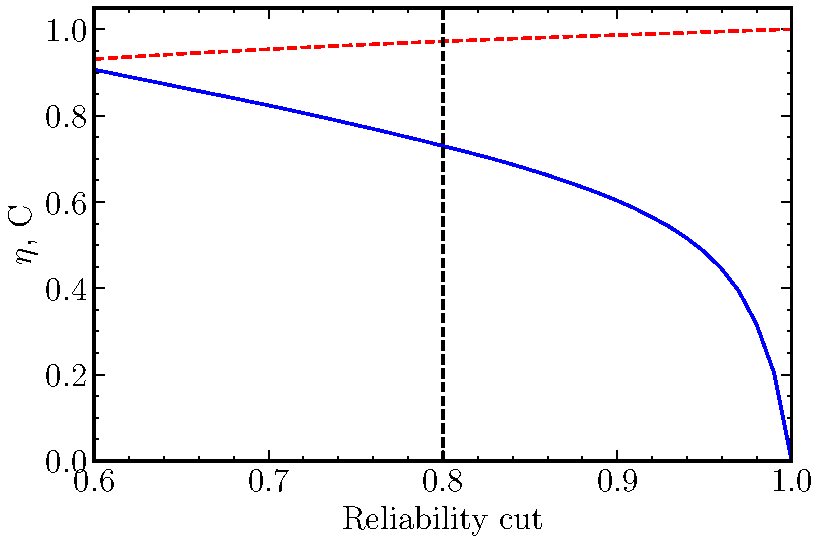
\includegraphics[width=\columnwidth]{Figures/completeness_and_cleanness.pdf}
	\caption{The completeness, $\eta$, and cleanness, C, of the SGP sample as a function of various minimum cuts in reliability, illustrated as solid blue and red dashed lines respectively. The vertical dashed line reprents the reliability cut used in all H-ATLAS fields (R $\geq$ 0.8).}
	\label{fig:completeness_and_cleanness}
\end{figure}

\section{Properties of \textit{Herschel} Sources and their Counterparts}

In the subsequent sections I report on the bulk properties of the SMGs in the SGP field that can be obtained from a combination of the sub-mm and near-IR data. While the far-IR to sub-mm wavebands unveil the dusty, cold regions of the Universe, the inclusion of the near-IR data (the $K_s$-band covers wavelengths between $\sim$ 2--2.3\,\micron) samples the peak of the emission of older stars and as such is suited for examining the stellar properties of a galaxy such as its stellar mass as it traces the total stellar content of a galaxy (\citealt{Cole_2001}; \citealt{Bell_2003}). Moreover, at high redshifts (z $\gtrsim$ 0.5) the rest frame optical bands are observed in the near-IR, meaning that the VIKING counterparts at higher redshifts also probe young stellar populations.

\subsection{Submillimeter Colours}
% Include a comparison of sub-mm colours across the data releases
\subsection{Near-IR Properties of \textit{Herschel} Sources}
% Include a comparison of magnitude distributions

\subsection{Multiplicity of Counterparts}
One important disadvantage to using the LR method to identify multiwavelength counterparts to low resolution sources is that it assumes a one-to-one matching of sources and counterparts. Given that we are restricted to a user defined reliability threshold for our sample, and that the sum of reliabilities for all possible candidates to a source may not exceed one, our reliable sample becomes biased against multiple systems, such as merging galaxies, members of a cluster or non-physical associations such as confusion due to blending, as their combined reliabilities reduces the maximum reliability of the chosen ID. For example, consider two galaxies that form part of a cluster that are observed with VIKING close to a SPIRE source. It is reasonable to imagine that these two sources may have similar K-band magnitude and radial offset from the source, and particularly if they are close to the sub-mm emission, may both have high likelihoods. In such a case, either source may be considered the true ID to the source (and in reality both are likely associated), but the use of Equation \ref{eq:reliability_multiple_counterparts} to define their reliabilities leads to the following simplification (assuming the likelihoods are much larger than $1-Q$):

\begin{equation}
    R_j \sim \frac{L_j}{\sum_i L_i} \sim \frac{L_j}{2L_j} \sim 0.5.
\end{equation}

In this scenario, neither counterpart would be considered the true ID and thus we are biased against multiple systems. 

In Table \ref{tab:multiplicity} I show the number of SPIRE sources and the fraction of those with reliable counterparts as a function of the number of possible candidates observed within 15". We observe that the fraction of sources with reliable counterparts decreases with increasing multiplicity. This suggests that the sample is in part incomplete because we miss sources where there is more than one genuine counterpart. In Figure \ref{fig:multiplicity} I show the reliable fraction of sources as a function of multiplicity for the SGP compared with previous H-ATLAS data releases in other fields. Comparing to the Science Demonstration Phase (\citealt{Fleuren_2012}), GAMA (\citealt{Bourne_2016}) and the NGP (\citealt{Furlanetto_2018}), we see that reliability fraction declines more slowly, peaks at slightly higher average $N_{\textrm{Match}}$ and is lower for sources where there is only a single possible counterpart. These effects are most likely a result of the increased search radius of 15" used during the SGP analysis compared to 10" in the other fields, which per source equates to a 2.5 factor increase in the search area ($A_{\textrm{SGP}}/A_{\textrm{Other}} = \pi r_{\textrm{SGP}}^2/\pi r_{\textrm{Other}}^2 = 225\pi/100\pi = 2.5$). The increased $r$ means that we are more likely to observe a reliable counterpart, but also means we increase the probability of matching erroneously to a background source, which would explain why we observe a higher false identification rate for the reliable sample of the SGP. The low fraction of reliably matched sources at $N_{\textrm{Match}} = 1$ may be due to an increase in unassociated VIKING objects being selected as the true ID. Occassionally, the chosen ID will be unassociated with the sub-mm source, but selected solely for being the only possible candidate despite having a large radial offset. This effect is more pronounced for an increase in $r$. In Table \ref{tab:multiplicity} we see that the average offset between VIKING galaxy and source is substantially higher when the galaxy is the only possible candidate, suggesting that some fraction of these sources are erroneously matched. However, the shift of the peak to higher $N_{\textrm{Match}}$ is likely due to the greater ability to discern between true IDs and chance alignments when the same number of candidates are spread over a larger surface area. Another reason why the reliable fraction is so low for $N_{\textrm{Match}} = 1$ is that a large fraction of the stellar candidates will fall in this bin as stars tend to be isolated (\citealt{Bourne_2016}) and therefore reduce the average reliability of these sources. Lastly, the increase in the search area around each SPIRE source means that the fraction of reliably matched sources does not fall until much higher $N_{\textrm{Match}}$, leading to a flatter distribution.


\begin{table}
    \centering
    \begin{tabular}{|p{2.5cm}|p{2.5cm}|p{2.5cm}|p{2.5cm}|p{4cm}|}
        \hline
        $N_{\textrm{Match}}$ & $N_{\textrm{SPIRE}}$ & $N_{\textrm{Reliable}}$ & Percent & Av. Separation [arcsec] \\
        \hline
        \hline
        0 & 2,739 & 0 & 0 & 0 \\
        1 & 11,692 & 5,477 & 47 & 6.3 \\
        2 & 24,268 & 14,568 & 60 & 4.7 \\
        3 & 32,948 & 20,396 & 62 & 4.1 \\
        4 & 33,526 & 20,383 & 61 & 3.8 \\
        5 & 27,745 & 16,359 & 59 & 3.6 \\
        6 & 20,236 & 11,563 & 57 & 3.4 \\
        7 & 12,999 & 7,155 & 55 & 3.4 \\
        8 & 8,079 & 4,355 & 54 & 3.3 \\
        9 & 4,983 & 2,640 & 53 & 3.4 \\
        10 & 3,017 & 1,643 & 54 & 3.3 \\
        \hline
    \end{tabular}
    \caption{The reliable fraction illustrated as a function of the number of candidates observed per source. From left to right the columns contain: the number of possible candidates per source; the number of SPIRE sources that have the number of candidates specified in column one; the number of those sources whose best counterpart has a reliability greater than 0.8; the reliable fraction given as a percentage; and the average separation between the chosen ID and the source in arcsec.}
    \label{tab:multiplicity}
    \end{table}

\begin{figure}
    \centering
    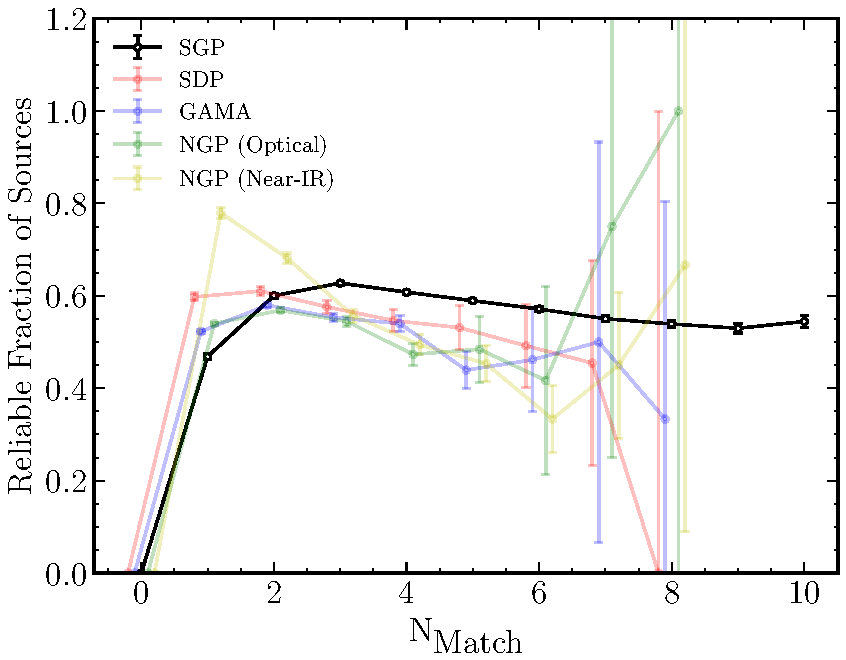
\includegraphics[width=\columnwidth]{Figures/multiplicity.pdf}
    \caption{The fraction of \textit{Herschel} sources with reliably matched counterparts as a function of the number of observed candidates. The results from various H-ATLAS fields are shown as the following lines: SGP (black, this work); SDP (red, \citealt{Smith_2011}); Phase 1 GAMA9 Field (blue, \citealt{Fleuren_2012}), GAMA (green, \citealt{Bourne_2016}), NGP (optical in yellow, near-IR in pink, \citealt{Furlanetto_2018}). All other works used a maximum search radius of 10" while the SGP analysis used 15". For clarity each line has been offset in $N_{\textrm{Match}}$ by a different value.}
    \label{fig:multiplicity}
\end{figure}

We can estimate the number of sources that have multiple genuine associations that were missed by the LR method by assuming that all candidates are associated with a single source if their combined reliabilities is greater than 0.8, but are missed because no individual counterpart meets the threshold. I find [...]\todo[color=orange]{Do calculation} such sources, however, due to the increased maximum $r$ and consequently increased average number of candidates per source, even moderately valued $R$ counterparts combine to exceed the reliability cut. Alternatively, we could use the likelihood values, $L$, for each counterpart, rather than their reliability as the likelihood has no upper limit unlike the bounds on reliability, $R \in [0, 1]$. From Equation \ref{eq:reliability_multiple_counterparts} a reliability of 0.8 or greater corresponds to $L > 0.66$, assuming a single candidate and a value of $Q = 0.835$. An estimate for the number of lost sources with multiple associated counterparts can be made assuming that a source with a best matched counterpart with $L > 0.66$ but $R < 0.8$ is influenced by nearby candidates. I find 33,967 sources that satisfy these conditions. However, this is likely an overestimate of the true number as a large fraction of these IDs will be due to a mixture of true mergers or close groups and chance alignments; a measure for the probability that two or more counterparts are physically associated is required to potentially identify galaxy groups or mergers.

An improved estimate that removes chance alignments can be made considering the photometric redshifts of the VIKING objects (the method of obtaining photometric redshifts for the VIKING sample is presented in Section \ref{sec:phot_z_VIKING}). As shown in \citealt{Fleuren_2012}, chance matches along the line of sight can be ruled out by comparing the redshifts of all possible matches, and considering them to be associated if they fall within $\sim$ 10\% of each other for photometric redshifts or $\sim$ 5\% if using spectroscopic redshifts. While this is a simple and effective method, it does not rule out sources that happen to lie on a similar line of sight to unrelated groups or mergers of galaxies (and the true ID remaining unmatched or beyond the VIKING survey limit). In the following, I describe a new method in which we use the background distribution of VIKING sources (as used for estimating the magnitude distribution of true counterparts in Section \ref{sec:true_counterparts_distribution}) to estimate the probability that a pair of VIKING galaxies with similar redshifts are associated with the sub-mm source. 

Firstly, I restrict both the SGP and background catalogues to contain only sources with two or more counterparts and I restrict this further to counterparts found within 8", as this is where the majority of $L > 0.66$ counterparts are found, reducing the chance of selecting pairs of galaxies that are unrelated to the source. For each position in both catalogues, I identify the pair of galaxies with the closest redshifts and calculate the difference in their redshifts divided by the error in the difference, i.e. $\Delta z/\sigma_{\Delta z}$. In Figure \ref{fig:delta_z_multiplicity} I show the probability distribution functions (PDFs) of $\Delta z/\sigma_{\Delta z}$ for the SGP catalogue (red line) and the background catalogue (black line). When a background subtraction of the SGP catalogue is made, we observe an excess close to $\Delta z = 0$ (blue line) where the area of this peak represents the probability that a close pair of VIKING galaxies is indeed related to the SPIRE source. I fit a Gaussian profile to the excess and calculate this probability to be 2 -- 5\% depending on the size of the bins used to generate the PDFs. By multiplying this probability by the total number of SPIRE sources for which we observe a close pair of VIKING galaxies, in this case we take this to be the width of the peak, $-0.1 \lesssim \Delta z/\sigma_{\Delta z} \gtrsim 0.1$, I find an estimate for the number of \textit{Herschel} sources with genuine multiple counterparts of $\sim$ 400 -- 1,000.

\begin{figure}
    \centering
    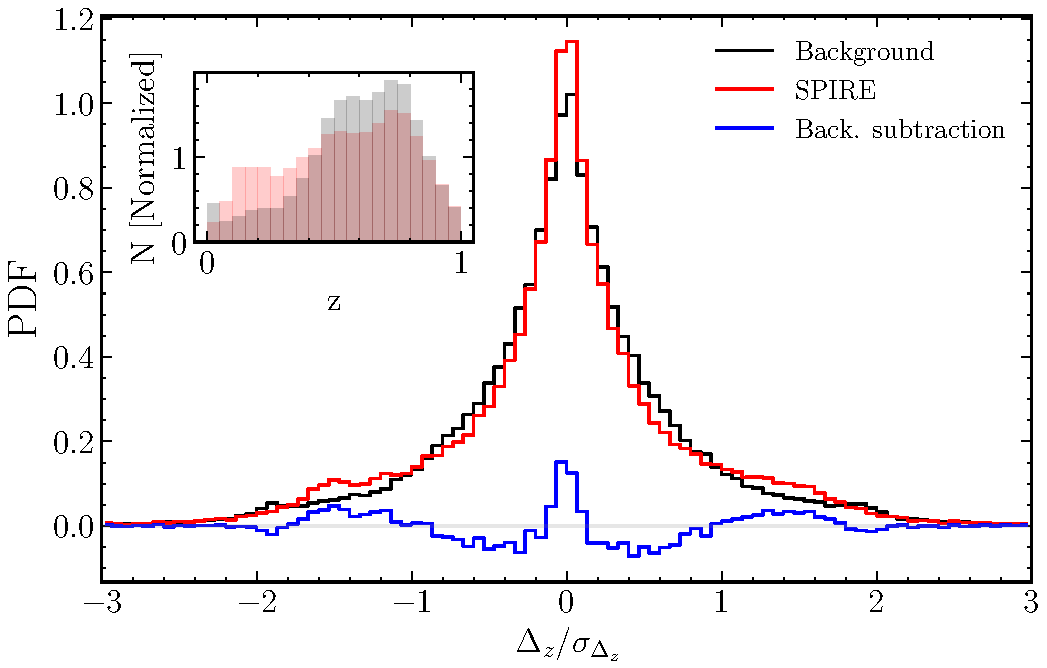
\includegraphics[width=\columnwidth]{Figures/delta_z_multiplicity.pdf}
    \caption{Probability distribution functions of $\Delta z/\sigma_{\Delta z}$, the difference between photometric redshifts of VIKING counterparts divided by the error in their difference, for pairs of galaxies located near 250\,\micron positions (within 8") in the SGP catalogue (red histogram) and near randomly located positions (black histogram). The blue histogram represents a background subtraction of the former. The excess located at $\Delta z = 0$ represents the subset of VIKING galaxy pairs with similar redshifts that are associated with the SPIRE source. The inset figure shows the normalized redshift distribution of VIKING counterparts observed within 8" of 250\,\micron positions in red and random positions in grey.}
    \label{fig:delta_z_multiplicity}
\end{figure}

It should be noted that this method is independent of the LR method and the resulting reliability values, and so the pair of VIKING objects chosen for each source does not always contain the candidate with the highest reliability. In total there are 70,880 sources where we observe two or more candidates with estimated photometric redshifts (within 8" of the source), of which approximately three quarters have best counterparts that are also part of the "redshift pair". The selected pairs for the remaining quarter of sources may be the locations of unassociated galaxy interactions or multiple systems related to the sub-mm source that is overlooked by the one-to-one matching of the LR method. The subset used here is approximately one third of all sources in the SGP (70,880/193,527) and so we expect mant more galaxy interactions and groups to be in the full SGP catalogue. We also note that the fraction accounting for all sources may be higher as there is evidence to suggest that the merger rate of galaxies evolves with redshift and reaches a peak at $z \sim 1.2$ (e.g. \citealt{Bell_2006}; \citealt{Ryan_2008}). If this is true, then a large fraction of interacting systems may be those beyond the VIKING detection limit and therefore lie in the blank SPIRE fields.

\subsection{Photometric Redshifts of Submillimeter Sources}
\label{sec:phot_z_Herschel}

Any study on the evolution of fundamental properties of extragalactic sources requires an estimate for the age of the galaxy and therefore its redshift. Having crossmatched the sources detected on the sub-mm images with the sources on the VIKING images, we can begin to construct spectral energy distributions (SEDs) that places constraints on the stellar properties as well as the dust emission. 

The dust emission can be well approximated using a two-temperature modified blackbody model (see Section [...]\todo[color=green]{Add reference to blackbody functions when written} for a more detailed description on modified blackbody functions). A characteristic SED that can be used to approximate the SED of a typical H-ATLAS source is presented in \citealt{Pearson_2013} and takes the form:

\begin{equation}
    S_\nu = A[B_\nu(T_{\textrm{hot}})\nu^\beta + \alpha B_\nu(T_{\textrm{cold}})\nu^\beta],
\label{eq:pearson_sed_model}
\end{equation}

where $S_\nu$ is the flux density of the source at the rest frame frequency, $\nu$, $A$ is a normalization factor, $B(T)$ represents the Planck function at temperature $T$, of which we assume two dust temperatures, $T_{\textrm{hot}}$ and $T_{\textrm{cold}}$, $\beta$ is the dust emissivity index and $\alpha$ represents the fraction of cold dust mass to hot dust mass. Using a sample of 40 H-ATLAS sources with spectroscopic redshifts, the optimal set of parameters were measured to be $T_{\textrm{hot}} = 46.9$\,K, $T_{\textrm{cold}} = 23.9$\,K and $\alpha = 30.1$ (assuming a fixed $\beta = 2$). This leaves a model with only two free parameters, the normalization and the redshift; a necessary simplification given that each source had at most three flux densities at the central wavelengths of the SPIRE bands (the PACS 100 and 160\,\micron flux densities were not included as the \textit{Herschel} images are less sensitive at these wavelengths). For each source the normalization and redshift were varied until a minimum chi squared was reached:

\begin{equation}
    \chi^2 = \sum_i \frac{S_i - S_{i,m}}{E_i^2},
\end{equation}

where $S_i$ is the flux density at each SPIRE wavelength, $i$, $S_{i,m}$ is the model prediction of the flux and $E_i$ is the error on the flux at wavelength $i$. 

While all sources in the SGP have estiamtes for their flux and flux errors at the SPIRE wavelengths in the second data release, the errors do not account for calibration errors.

\subsection{Photometric Redshifts of VIKING Counterparts}
\label{sec:phot_z_VIKING}

%\subsection{Comparison between H-ATLAS Data Releases}
% Include correlations with redshift now they have been described (e.g. flux and magnitude against redshift)
% Include a description of the full H-ATLAS: a legacy product that has no plans for being replaced
%\section{Gravitational Lensing in the SGP}
%\subsection{The Brightest Lenses}
%\subsection{Extending the Search for Lenses to Lower Fluxes}
\listoftodos

\chapter{Redshift Evolution of the Dust Mass Function}
\label{chapter:Dust_Mass_Functions}
\sloppy

\section{Introduction}

As discussed in Chapter \ref{chapter:Introduction}, dust is composed of metals that are produced from stellar nucleosynthesis, and then expelled into the ISM via supernovae and stellar winds. While some fraction of these metals mix with the gas phase in the ISM, around $30 - 50\%$ of the metals condense into dust grains (\citealt{Draine_2007b}). If this fraction of metals that get locked up in dust grains is somewhat consistent over time, then dust may be considered a useful tracer of gas metallicity in a galaxy. For this reason, the total dust mass is a fundamental property of the ISM that can be used to study the evolutionary stage of the galaxy (e.g. \citealt{Cortese_2012, deVis_2017a, deVis_2017b}). Moreover, dust is not just the product of previous star formation, but also, as the site of molecule formation like $H_2$, it has a significant influence on the formation of molecular clouds for future star formation. Understanding the dust content of galaxies over cosmic time is therefore important in providing insight into the evolution of galaxies and their ISM. In this Chapter, we estimate the dust masses of the galaxies in the South Galactic Pole field and derive the far-IR selected dust mass function (DMF), the space density of galaxies as a function of dust mass, in redshift slices of width $0.2$ out to $z = 1$.

\section{Local and High Redshift DMFs in the Literature}

%Using surveys selected from far-IR/sub-mm wavelengths provides a number of advantages when determining the DMF. At longer sub-mm wavelengths we sample the Rayleigh-Jeans tail of the Planck function where the flux density is least sensitive to the temperature of the dust and most sensitive to the dust's mass. Prior to the surveys conducted with \textit{Herschel}, \textit{Planck} and SCUBA in the local Universe, estimates of the local DMF often started from local \textit{IRAS} 60\,\micron\ luminosity functions (LF) and extrapolating this to sub-mm wavelengths on the assumption of an average far-IR SED with a single dust temperature and dust emissivity index $\beta$ for all galaxies. Naturally, this lead to strong dependency on the assumed dust temperature and $\beta$ value. Given that temperature evolves with luminosity (see our study on the temperature evolution with redshift for dusty star forming galaxies, DSFGs; Figure \ref{fig:t_evolution}), extrapolating from one wavelength to another inherently contained a bias at high and low luminosity scales, causing a distortion in any DMF measured from the translation of the luminosity function (\citealt{Dunne_2000}). The advent of \textit{Herschel} and \textit{Planck} allowed for large samples to be detected at far-IR wavelengths closer to the peak of the dust emission, enabling estimates of the DMF directly from sub-mm wavebands. The main disadvantage of these long wavelength derived DMFs is the large beam size at these wavebands, causing blending and source misidentification (as illustrated in our use of the Likelihood Ratio method in the previous chapter).

The first direct measurements of the far-IR/sub-mm derived DMF were with SCUBA using the SCUBA Local Universe Galaxy Survey \mbox{(SLUGS: \citealt{Dunne_2000, Dunne_2001, Vlahakis_2005})}, a survey of local \textit{IRAS}-selected galaxies. However, these studies were limited by small number statistics and were typically limited to very small redshifts. A high redshift ($z = 2.5$) DMF for comparison was presented in \citealt{Dunne_2003}, suggesting that galaxies with the highest dust masses have an order of magnitude more dust than locally (assuming pure dust mass evolution and no evolution in the number density of the most massive galaxies). Improvements were made with the introduction of BLAST, which allowed for the derivation of the DMF from a sample of galaxies selected at wavelengths spanning the peak of the far-IR spectrum (the same wavelengths as the \textit{Herschel}-SPIRE instrument). \citealt{Eales_2009} used BLAST data to arrive at similar conclusions, that there is strong evolution in both the $250\,\mu$m luminosity function (LF) and in the DMF out to $z = 1$. The concurrence of the two suggesting that the evolution in the far-IR/sub-mm luminosity of these galaxies is directly related to the increase in the size of their dust reservoirs. However, this study was also limited by small number statistics ($\sim 100$ sources).

The first study to measure the evolution in the DMF using the large area of H-ATLAS was \citealt{Dunne_2011}, using a $250\,\mu$m selected sample of $1,867$ sources from the Science Demonstration Phase (SDP). This represented a sample an order of magnitude larger than previous studies, allowing for a significant direct measurement of the space-density of galaxies as a function of dust mass, out to a redshift of $0.5$. As we explored in the previous Chapter, the upper redshift limit of this study was set by the limiting magnitude of the optical surveys in the \textit{Herschel} fields. The main finding from this study was that the integrated dust density of the Universe, that is the total dust mass in a given cosmological volume, evolves with redshift according to $\rho_{\textrm{dust}} \propto (1+z)^{4.5}$ between $0 < z < 0.5$. The local density was estimated to be $\rho_{\textrm{dust}, (z=0)} = 9.8\times10^4$\,$M_\odot$Mpc$^{-3}$. This work was further developed in \citealt{Beeston_2018} by deriving the local ($z < 0.1$) DMF for the largest sample of galaxies at the time of writing ($\sim 16,000$ galaxies), utilizing the aforementioned crossmatching between the H-ATLAS and the GAMA spectroscopic survey detailed in \citealt{Bourne_2016}. The sample size of \citealt{Beeston_2018} permitted signifcant numbers of galaxies with dust masses as low as $\sim 10^4\,M_\odot$ and therefore extended the observed mass range by at least an order of magnitude compared to previous measurements. This gave better constraints on the low mass end of the DMF which, despite accounting for a negligible amount of the dust budget compared to the most massive galaxies, contribute substantially in number. This low mass regime is constrained by sources that tend to be nearby and faint, and suffer from low numbers in flux-limited surveys such as H-ATLAS, thus this study provides important measurements in an otherwise uncertain region of the DMF. Given the size of the \citealt{Beeston_2018} sample the measurement of the low mass end of the DMF in this study is currently our best estimate. Despite differences in the measured number density of low mass galaxies, \citealt{Dunne_2011} and \citealt{Beeston_2018} both have local dust mass densities (DMD) in good agreement. More recently, \citealt{Driver_2018} produced an extended DMF and measured the DMD out to $z = 5$. This study was based on an optically-selected sample of approximately $570,000$ galaxies from GAMA, G10-COSMOS (\citealt{Davies_2015}; \citealt{Andrews_2017}) and 3D-HST (\citealt{Brammer_2012, Momcheva_2016}). Unlike \citealt{Dunne_2011}, this study found no evidence for a strong evolution in the dust content of galaxies in the past $5\,$Gyr, instead observing a flat DMD since $z = 0.5$. However, an apparent evolution is observed in the dust luminosity which would suggest that a strong evolution in dust temperature is required in order to maintain a flat DMD. Other notable works that measure the evolution of the DMF to high redshifts include \citealt{Pozzi_2020} and \citealt{Dudzeviciute_2021}. The former derived the DMF from $z \sim 0.2$ to $z \sim 2.5$ using a $160\,\mu$m \textit{Herschel}-PACS selected catalogue of approximately $5,300$ galaxies in the COSMOS field. In accordance with \citealt{Driver_2018}, they find a peak in the redshift evolution of the DMD at $z \sim 1$, but more in keeping with \citealt{Dunne_2011}, they also observe a decreasing trend from the peak in dust density to the present day. The implication of such varied results is that consistency among studies depends largely on the selection wavelength of the sample, the survey area and any assumptions that may be made during the measurement of the dust masses of the galaxies. We note that of the studies mentioned here, the sample of \citealt{Pozzi_2020} is selected from the shortest wavelength ($160\,\mu$m), which may explain some of the differences observed between this study and the other, \textit{Herschel}-selected samples. This will be explored further in Section \ref{sec:schechter_functions}. Finally, \citealt{Dudzeviciute_2021} add valuable constraints on the DMF at $z = 1 - 2$ and $z = 3 - 4$ based on two samples selected at wavelengths corresponding to nearly indentical rest frame $\sim 180\,\mu$m populations. Between $1 < z < 2$, \citealt{Dudzeviciute_2021} studied the dust properties of $121$ SMGs from the $450\,\mu$m SCUBA-2 Ultra Deep Imaging EAO Survey (STUDIES: \citealt{Wang_2017, Chang_2018, Lim_2020b, Lim_2020c}) and compared these results to an $850\,\mu$m SMG sample with redshifts between $3 < z < 4$ from the ALMA/SCUBA-2 Ultra Deep Survey (AS2UDS: \citealt{Stach_2018, Stach_2019, Dudzeviciute_2020}). 

In this study, we derive the DMF from the galaxies observed in the H-ATLAS SGP field presented in Chapter \ref{chapter:Data_Release_3}. We include in our study those galaxies matched with high reliability ($R > 0.8$) to a VIKING counterpart with an estimated redshift from the HELP catalogue. The dust masses are calculated from the \textit{Herschel}-SPIRE $250\,\mu$m flux densities, and thus our estimates of the DMF are likely to follow similar observed trends as in the previous H-ATLAS studies of \citealt{Dunne_2011} and \citealt{Beeston_2018}. The work presented here allows us to expand on these works by extending the \textit{Herschel} predicted DMF to higher redshifts as a result of the increased depth from the near-IR crossmatching. In addition, we implement an error analysis that propagates errors in the photometric redshifts through to the final DMF, allowing us to use a sample devoid of spectroscopic redshifts. The spectroscopic coverage of the SGP is much lower than for the GAMA fields, but by propagating the photometric redshift errors through our analysis, we can define a signifcantly sized sample of galaxies, providing they fulfill three criteria: i) they are classified as galaxies (Section \ref{sec:star_galaxy_classifier}), ii) they have a near-IR counterpart that has been matched with a high probability, and iii) have an associated redshift. We shall use the photometric redshifts from the \textit{Herschel} Extragalactic Legacy Project (HELP, Section \ref{sec:phot_z_VIKING}). This corresponds to a sample of $81,895$ galaxies, making it the largest sample of \textit{Herschel} galaxies used to study the dust content of the Universe.

\section{Dust Properties of H-ATLAS Galaxies}

To measure the dust masses of our SGP galaxies, we require observations from the same rest frame wavelengths, regardless of their redshift. With select \textit{Herschel} wavebands to work with, we must be able to k-correct their dust spectra to a given rest frame wavelength. This in turn requires us to have an understanding of what a typical dust SED might look like at all far-IR wavelengths. Although galaxies contain dust with a range of temperatures, previous studies have shown that most interstellar dust grains have a cold temperature of $\sim 20\,$K (e.g. \citealt{Dunne_2001, Vlahakis_2005, Draine_2007a, Boselli_2010, Smith_2012b, Smith_2013}). Dust close to sources of heating such as star forming regions and AGN have higher temperatures and radiate at rest frame wavelengths $\lesssim 100\,\mu$m. These grains can influence the temperature measured from an isothermal dust model. To account for this mixing of dust temperatures, the ideal scenario would be to estimate the dust mass of a galaxy using a mass-weighted temperature of the dust. This would require fitting a model with multiple different dust temperatures and weighting the temperatures by the mass of the dust for that component. We observed such an example earlier when we described the H-ATLAS galaxies using the two-temperature model of \citealt{Pearson_2013}. However, it has already been shown that the cold dust reservoir at $\sim 20\,$K has the most signifcant contribution by mass (\citealt{Pearson_2013}) and the difference between the mass weighted dust temperature and the isothermal temperature is often not significant (e.g. \citealt{Clark_2015}). For example, if we assume that H-ATLAS galaxies are well approximated by the two temperature model of \citealt{Pearson_2013} (where $T_{\textrm{hot}} = 46.9\,$K, $T_{\textrm{cold}} = 23.9\,$K and $\alpha = M_c/M_h = 30.1$), then the mass weighted temperature is given by $T_{\textrm{dust, weighted}} = (M_cT_c + M_hT_h)/(M_c + M_h) \approx 24.6\,$K, which is only marginally warmer than the cold dust component.

In addition, to include hot dust at $\lambda_{\textrm{rest}} \lesssim 100\,\mu$m, we would require short wavelength photometry (presumably from PACS) with signifcant SNR to be able to put meaningful constrains on this temperature component. As shown in Table \ref{tab:snr_fraction}, the percentage of galaxies in our sample that have significant detections at the PACS wavelengths decreases rapidly with redshift to as low as $\sim 6 - 8\%$ by just $z \sim 0.3$. With so few galaxies in our redshift range having PACS detections with useful SNR, the ability to adequately fit an SED to the \textit{Herschel} observations is essentially the same whether we are considering an isothermal or multi-component model. The benefit of assuming an isothermal model in this instance is the reduction in the number of model parameters.

\begin{table}
    \centering
    \begin{tabular}{p{3cm}|p{1.75cm}|p{1.75cm}|p{1.75cm}|p{1.75cm}|p{1.75cm}}
        \hline
        \hline
        Redshift Interval & 100\,\micron & 160\,\micron & 250\,\micron & 350\,\micron & 500\,\micron \\
         & [> 3$\sigma$] & [> 3$\sigma$] & [> 4$\sigma$] & [> 4$\sigma$] & [> 4$\sigma$] \\
        \hline
        \hline
        0 < z < 0.2 & 22.6 & 28.0 & 99.3 & 31.4 & 5.0 \\
        0.2 < z < 0.4 & 6.0 & 7.8 & 98.6 & 20.3 & 2.7 \\
        0.4 < z < 0.6 & 3.0 & 4.4 & 96.9 & 28.1 & 4.6 \\
        0.6 < z < 0.8 & 1.4 & 2.8 & 96.0 & 37.5 & 6.7 \\
        0.8 < z < 1 & 0.9 & 2.1 & 95.3 & 45.0 & 8.0 \\
        \hline
    \end{tabular}
    \caption[The significance of \textit{Herschel} observations in redshift slices to $z = 1$]{The percentage of sources in our galaxy sample that have detections in each \textit{Herschel}-PACS and \textit{Herschel}-SPIRE waveband at the level of significance indicated in the column headers. The percentages are shown for redshift bins of width $0.2$, the same used for deriving the binned dust mass functions.}
    \label{tab:snr_fraction}
\end{table}

Without sufficient data to constrain the dust temperature and $\beta$ simultaneously, we assume a fixed $\beta = 2$ and fit an isothermal modified blackbody to all galaxies. In Figure \ref{fig:dust_temperatures} we plot the distribution of measured dust temperatures as a function of photometric redshift. We see that the median value at all redshifts is consistent with $20\,$K, which we shall assume herein as the typical temperature of the cold ISM. The righthand panel of Figure \ref{fig:dust_temperatures} shows the distribution of dust temperatures (black histogram) and the contributions from galaxies with one (red), two (blue) and three (green) SPIRE observations with flux densities at greater than $4\sigma$ significance. As previously shown by \citealt{Beeston_2018} the galaxies with significant \textit{Herschel} fluxes in all three SPIRE wavebands are on average colder than those with only one or two bands. This illustrates a simple selection effect of the \textit{Herschel} observations. If a galaxy is detected at $250\,\mu$m, then it is more likely to also have detections at longer wavelengths if the dust is colder than average (the far-IR SED shifts to longer wavelengths at colder dust temperatures).

\begin{figure}
	\centering
	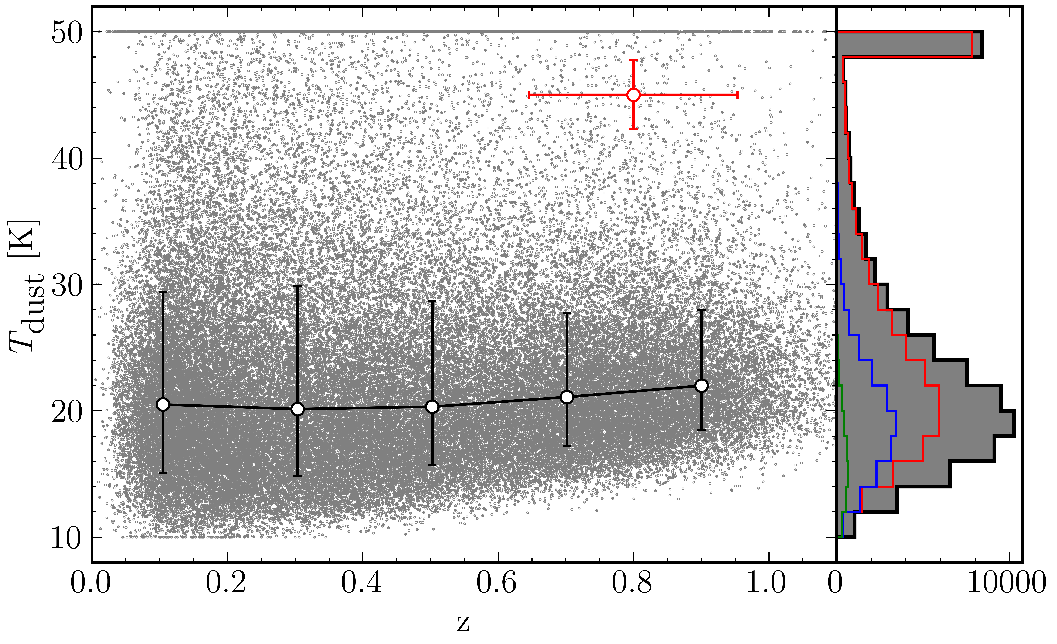
\includegraphics[width=0.8\columnwidth]{Figures/dust_temperatures.pdf}
	\caption[The distribution of dust temperatures as a function of redshift]{The dust temperature against redshift for galaxies in the SGP field. The red cross illustrates the typical $1\sigma$ error in the redshifts and dust temperatures. The black error bars represent the median dust temperature in each redshift bin, along with the $1\sigma$ range in the distribution ($16$th to $84$th percentiles). The righthand panel shows the histogram of dust temperatures for all galaxies (grey filled), galaxies with SNR $> 4$ in one band (red), in two bands (blue) and in three bands (green).}
	\label{fig:dust_temperatures}
\end{figure}

In the next section we shall start from the assumption that the dust spectrum of all galaxies in our sample can be approximated by an SED with a characteristic dust temperature of $20\,$K when deriving the DMF (e.g. \citealt{Vlahakis_2005}). This knowledge is required for certain methods used to derive a binned DMF in $M_{\textrm{dust}}-z$ space as they rely on knowing the shape of the SED to apply appropriate k-corrections in each bin. As we shall explain later, some methods for calculating binned functions allow for each galaxy to use its own dust spectrum rather than a global SED to compute the required k-corrections. We shall discuss how this impacts our DMF in later sections.

We calculate dust masses from monochromatic rest frame luminosities, which we derive from the k-corrected observed flux densities at $250\,\mu$m. We translate the $250\,\mu$m flux densities of the SGP galaxies into monochromatic luminosities using

\begin{equation}
    L_{250} = \frac{4\pi D_L^2 S_{250}K}{(1+z)},
\label{eq:monohromatic_luminosities}
\end{equation}

\noindent where $L_{250}$ is in units of W Hz$^{-1}$, $D_L$ is the luminosity distance, $S_{250}$ is the observed flux density at $250\,\mu$m and $K$ is the k-correction that allows us to define a rest frame quantity at $250\,\mu$m in terms of the observed frame at the same wavelength, given by

\begin{equation}
    K = \frac{S_{250}^{K}}{S_{250}^{\textrm{obs}}} = \Bigg(\frac{\nu_{K}}{\nu_{\textrm{obs}}}\Bigg)^{3+\beta}\frac{e^{(h\nu_{\textrm{obs}}/kT)} - 1}{e^{(h\nu_{K}/kT)} - 1},
\label{eq:k_correction}
\end{equation}

\noindent where $\nu_{K} = \nu_{\textrm{obs}}(1+z)$ and $T$ and $\beta$ are the dust temperature and emissivity index describing the SED. 

Let us briefly consider a galaxy at the edge of our redshift range, $z \sim 1$. The factor $K$ allows us to convert $S_{250}^{\textrm{obs}}$, the emission radiated at $250\,\mu$m ($1.2\,$THz) and observed at $125\,\mu$m ($2.4\,$THz) to $S_{250}^{K}$, the $250\,\mu$m flux density in the galaxy's rest frame. The monochromatic luminosity at $250\,\mu$m is then converted to a dust mass using

\begin{equation}
    M_{\textrm{dust}} = \frac{L_{250}}{4\pi\kappa_{250}B(\nu_{250}, T)},
\label{fig:dust_mass}
\end{equation}

\noindent where $\kappa_{250}$ is the dust mass absorption coefficient at $250\,\mu$m. The dust mass absoprtion coefficient is an amalgamation of terms including the efficiency with which the dust grains emit in reference to a perfect blackbody, the size of the dust grains and their mass volume density. As will be discussed in Chapter \ref{chapter:Dust_Evolution}, the frequency dependence of the absorption coefficient, $\kappa_\nu$, can be parameterized as a power law with an exponent of $\beta$, thus the value of $\beta$ naturally encodes the frequency dependence of these properties. For this reason, the value of $\kappa_\nu$ is highly uncertain with a wide range of values spanning multiple orders of magnitude being presented in the literature (\citealt{Clark_2019}). A commonly used value is $0.077\,$m$^2$kg$^{-1}$ at $850\,\mu$m (\citealt{Dunne_2000, daCunha_2008, Dunne_2011}) which represents a theoretical value lying between the expected value for graphite and silicate dust grains (\citealt{Draine_1984}). Assuming $\beta = 2$ we scale this value to $250\,\mu$m such that $\kappa_{250} = 0.89\,$m$^2$kg$^{-1}$.

\section{Sources of Incompleteness}

An important issue to consider when deriving our DMF is the completeness of our \textit{Herschel} survey and how we may account for missing galaxies when estimating the space-density of objects. In the following sections we outline the methods we use to estimate the incompleteness of our sample and thus the completeness correction factors we apply to our SGP catalogue, in order to account for sources we either do not observe or do not retain from the LR method described earlier. Each object in our SGP sample will be multiplied by correction factors that compensate for the number of times we might expect to observe this type of galaxy, based on the number of missing \textit{Herschel} sources and sources without a near-IR identification.

\subsection{\textit{Herschel} Catalogue Incompleteness}

The first correction factor is a direct result of the source extraction process used to create the \textit{Herschel} catalogues from the far-IR images. Due to source confusion these catalogues are incomplete as we approach the flux limit of the survey. To determine the completeness of the H-ATLAS catalogues, \citealt{Valiante_2016} used a catalogue of simulated sources embedded in real H-ATLAS maps to predict the efficiency of the \texttt{MADX} algorithm in recovering the sources. The completeness is shown as a function of the measured $250\,\mu$m flux density in Figure \ref{fig:submm_completeness} and is listed in Table \ref{tab:submm_completeness_table} along with the correction factors, $c_{\textrm{far-IR}}$, defined as the reciprocal of the completeness. We use an interpolated version of this table when applying the correction factors to our SGP galaxies. Unsurprisingly, the highest correction factors are found as we approach the flux limits of the survey where confusion noisce dominates and the likelihood of lost sources rises.

\begin{table}
    \centering
    \begin{tabular}{p{5cm}|p{2.5cm}|p{2.5cm}}
        \hline
        \hline
        $250\,\mu$m Flux Density [mJy] & Completeness & $c_{\textrm{far-IR}}$ \\
        \hline
        \hline
        20.0 & 0.541 & 1.849 \\
        26.5 & 0.762 & 1.313 \\
        35.1 & 0.903 & 1.107 \\
        46.4 & 0.969 & 1.032 \\
        61.5 & 0.989 & 1.011 \\
        81.4 & 0.993 & 1.007 \\
        107.7 & 0.997 & 1.003 \\
        142.6 & 0.997 & 1.003 \\
        188.8 & 0.997 & 1.003 \\
        250.0 & 0.999 & 1.001 \\
        \hline
    \end{tabular}
    \caption[Far-IR catalogue completeness as a function of $250\,\mu$m flux density]{The far-IR completeness and corresponding correction factors as a function of the measured flux density.}
    \label{tab:submm_completeness_table}
\end{table}

\subsection{Reliable ID Incompleteness}

The second correction function arises from our inability to identify the near-IR counterparts, with a sufficiently high reliability, for all the \textit{Herschel} sources for which we observed a counterpart on the VIKING image. The objects that we do not recover with $R < 0.8$ are largely the result of large positional uncertainties, the possibility of coincident background objects and multiple systems that are associated, but treated independently by the LR method. 

In its simplest form, the completeness of our reliable sample is defined as the redshift distribution of our IDs divided by the true redshift distribution of \textit{Herschel} counterparts, scaled to the number of sources for which we observe a nearby VIKING counterpart; $C_{\textrm{id}} = n_{\textrm{reliable}}(z)/n_{\textrm{real, scaled}}(z)$. This second term is closely related to the probability distribution of true counterparts as a function of redshift, $q(z)$, much like the true counterparts distribution we derived as a function of $K_s$-band magnitude in the previous Chapter. Using the same formalism as Equation \ref{eq:true_counterparts_distribution}, we define the denominator as

\begin{equation}
    n_{\textrm{real, scaled}} = q(z)\times N_{\textrm{250\,\micron}} = \frac{n_{\textrm{real}}(z)}{\sum_{z_i}n_{\textrm{real}}(z_i)}\times QN_{\textrm{250\,\micron}},
    \label{eq:n_real_scaled}
\end{equation}

\noindent where $n_{\textrm{real}}(z)$ is the redshift distribution of true counterparts (recall Equation \ref{eq:real_distribution}) and $N_{\textrm{250\,\micron}}$ is the number of $250\,\mu$m \textit{Herschel} positions. As previously, the required correction functions are the reciprocal of the completeness. When we derived the $q(m)$ distribution in Section \ref{sec:true_counterparts_distribution} we noted that the distribution is normalized such that the integal of $q(m)$ over all magnitudes up to the limiting magnitude of the VIKING survey is equal to the probability that the source is detected ($\int^{m_\textrm{lim}} q(m) dm = Q$). As an extension of this normalization, we recognize that the integral of the ID redshift distribution multiplied by the correction factors should give the total number of sources with observable counterparts (i.e. $\int_z c_{\textrm{id}} n_{\textrm{reliable}}(z) dz = QN_{\textrm{250\,\micron}}$, where $c_{\textrm{id}}$ are the correction factors given by $1/C_{\textrm{id}}$).

The ID completeness as a function of redshift is listed in Table \ref{tab:id_completeness_table} and illustrated in Figure \ref{fig:id_completeness} alongside the completeness functions from the SDP (\citealt{Smith_2011}), GAMA9 field (\citealt{Fleuren_2012}) and NGP (\citealt{Bourne_2016}). The average correction factor per source in the SGP is approximately two. Near the median redshift of the distribution ($z \sim 0.5$) the completeness is lower in the SGP than in other fields, though we note that we do not include spectroscopic redshifts, which might lower our completeness. The general trend for all H-ATLAS studies is a steady decline from $\sim 100\%$ completeness at $z = 0$ to a minimum at $z \sim 0.5 - 0.7$ followed by a rise at higher redshifts. The decrease towards $z = 0.5$ might be a result of a fixed search radius corresponding to a greater physical scale at larger cosmological distances. This would result in a greater probability of observing spurious counterparts that decrease the ID rate. Presently, we are not sure why the ID completeness rises again at higher redshifts, but one possible explanation is the greater probability of lensing events along the line of sight 

\begin{table}
    \centering
    \begin{tabular}{p{4.5cm}|p{2.5cm}|p{2.5cm}}
        \hline
        \hline
        Redshift & Completeness & $c_{\textrm{id}}$ \\
        \hline
        \hline
        0.05 & 0.984 & 1.016 \\
        0.15 & 0.881 & 1.135 \\
        0.25 & 0.713 & 1.403 \\
        0.35 & 0.542 & 1.844 \\
        0.45 & 0.432 & 2.313 \\
        0.55 & 0.387 & 2.581 \\
        0.65 & 0.372 & 2.685 \\
        0.75 & 0.360 & 2.776 \\
        0.85 & 0.392 & 2.552 \\
        0.95 & 0.422 & 2.369 \\
        \hline
    \end{tabular}
    \caption[ID completeness as a function of redshift]{The counterpart ID completeness and corresponding correction factors as a function of redshift.}
    \label{tab:id_completeness_table}
\end{table}

\begin{figure}
	\centering
	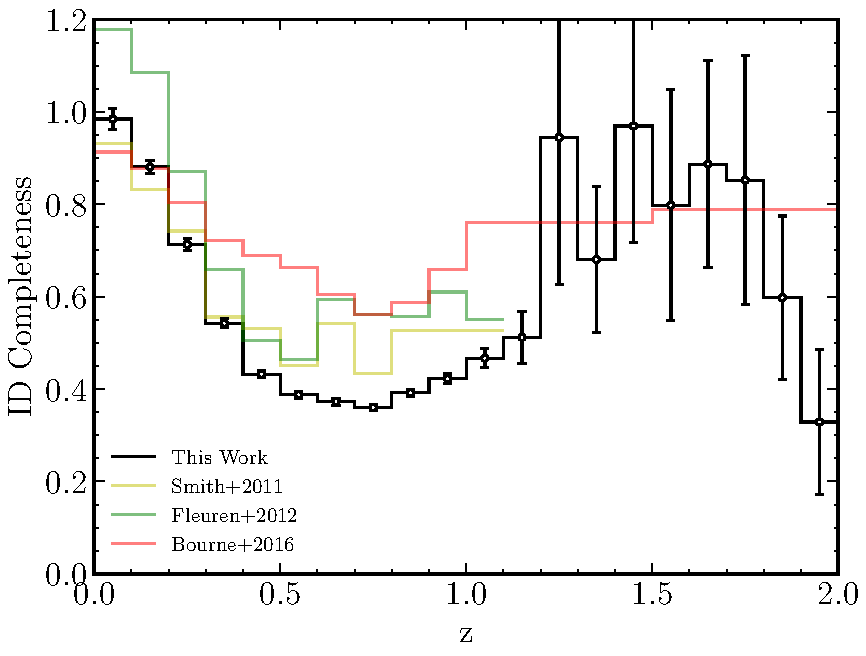
\includegraphics[width=0.8\columnwidth]{Figures/id_completeness.pdf}
	\caption[Completeness of our reliable SGP sample as a function of redshift]{The completeness of our $R > 0.8$ SGP sample as a function of redshift (black error bars), calculated using $n_{\textrm{reliable}}(z)/n_{\textrm{real, scaled}}$ where $n_{\textrm{real, scaled}}(z)$ is given by Equation \ref{eq:n_real_scaled}. Completeness functions from other H-ATLAS studies, \citealt{Smith_2011}, \citealt{Fleuren_2012} and \citealt{Bourne_2016}, are shown as yellow, green and red lines, respectively.}
	\label{fig:id_completeness}
\end{figure}

\section{Estimators of the Binned Dust Mass Function}
\label{sec:dmf_estimators}

The dust mass function, $\phi(M_{\textrm{dust}})$, represents the space density of galaxies as a function of dust mass, which in its differential form is given as the number of galaxies per unit comoving volume per unit dust mass interval

\begin{equation}
    \phi(M_{\textrm{dust}}, z) = \frac{d^2N}{dV dM_{\textrm{dust}}},
\label{eq:differential_phi}
\end{equation}

\noindent where $N$ is the number of galaxies with dust mass $M_{\textrm{dust}}$ observed in the comoving volume $V$ at redshift $z$. In this section we outline two methods of calculating the binned dust mass function; the ubiquitously used $1/V_{\textrm{max}}$ method \mbox{(\citealt{Schmidt_1968, Felten_1976, Avni_1980})} and the approximate method, $\phi_{\textrm{est}}$, proposed by \citealt{Page_2000}. Alternative parametric methods (e.g. the maximum-likelihood method of \citealt{Marshall_1983}) allow us to explore the entire $M_{\textrm{dust}} - z$ space, including regions that are not covered by observational data, and allow us to produce continuous functions for $\phi(M_{\textrm{dust}}, z)$. Although it is well established that the dust mass function can be parameterized in the form of a Schechter function (\citealt{Press_1974, Schechter_1976}), it is not obvious how this function evolves with redshift and which functional form should be used for this evolution. For this reason, we prefer to use binned, non-parametric methods and empirically study the redshift evolution of the DMF.

\subsection{The $1/V_{\textrm{max}}$ Method}

The prevalent use of the $1/V_{\textrm{max}}$ method stems from our need to overcome the Malmquist bias (\citealt{Eddington_1914, Malmquist_1922}) that causes selection biases in flux density limited samples. Malmquist bias refers to the tendency for flux-limited samples to be increasingly dominated by more luminous sources with increasing cosmological distance. As a result, more luminous objects are detected in larger volumes than less luminous objects, which needs to be accounted for in our space-density calculations. The $1/V_{\textrm{max}}$ method corrects for this bias by weighting each galaxy according to the maximum comoving volume in which it can be observed by the survey. The number density of galaxies in a given dust mass-redshift bin ($\Delta M_{\textrm{dust}} \Delta z$) is approximately given by the sum of the reciprocal of the maximum comoving volume for all galaxies in this bin

\begin{equation}
    \frac{dN}{dV} \sim \sum_{i=1}^N \frac{1}{V_{\textrm{max,i}}(M_{\textrm{dust,i}},z)},
\label{eq:number_density_1/v_method}
\end{equation}

\noindent where $V_{\textrm{max,i}}$ is the maximum comoving volume in which the $i$th galaxy in this bin could be detected by the survey. The volume is calculated according to

\begin{align}
    V_{\textrm{max},i}(M_{\textrm{dust,i}},z) &= \int^{\scriptscriptstyle \textrm{survey}} \int_{\scriptscriptstyle z_1}^{\scriptscriptstyle \textrm{min}[z_2, z(M_{\textrm{dust,i}},S_{\textrm{lim}})]} \frac{dV}{dz} dz d\Omega \nonumber \\
    &= \int^{\scriptscriptstyle \textrm{survey}} \int_{\scriptscriptstyle z_1}^{\scriptscriptstyle \textrm{min}[z_2, z(M_{\textrm{dust,i}},S_{\textrm{lim}})]} D_H \frac{(1+z)^2 D_A^2}{E(z)} dz d\Omega
\label{eq:volume_1/v_method}
\end{align}

\noindent where $\frac{dV}{dz}$ is the differential comoving volume given in the following line in terms of the Hubble distance, $D_H$, the angular diameter distance, $D_A$, and the dimensionless Hubble parameter, $E(z)$. The integration over redshift has limits from the bottom redshift of the bin, $z_1$, to either the upper edge of the bin, $z_2$, or the redshift beyond which the galaxy with dust mass $M_{\textrm{dust},i}$ would not be observed, whichever is smallest. A graphical illustration of the dust mass-volume space available to a galaxy with a dust mass $M_{\textrm{dust},i}$ is presented in the left-hand panel of Figure \ref{fig:volume_comparison}.

The binned dust mass function using this method is then defined by dividing the number density by the dust mass bin width (which we define in terms of logarithmic dust mass)

\begin{equation}
    \phi_{1/V}(M_{\textrm{dust}},z) = \frac{1}{\Delta \textrm{log}_{10}(M_{\textrm{dust}})} \sum_{i=1}^N \frac{1}{V_{\textrm{max,i}}(M_{\textrm{dust,i}},z)}.
\label{eq:phi_1/v_method}
\end{equation}

To account for the incompleteness of the sample, we include the correction factors we derived in the previous section in the following way

\begin{equation}
    \phi_{1/V}(M_{\textrm{dust}},z) = \frac{1}{\Delta \textrm{log}_{10}(M_{\textrm{dust}})} \sum_{i=1}^N \frac{c_{\scriptscriptstyle \textrm{far-IR}} c_{\scriptscriptstyle \textrm{id}}}{V_{\textrm{max,i}}(M_{\textrm{dust,i}},z)}.
\label{eq:phi_1/v_method}
\end{equation}

While this method suitably deals with Malmquist bias and does not require an a-priori analytic form, it can produce unwanted artefacts when applied to flux-limited samples. The problem arises when we have an uncertain estimate of the $250\,\mu$m flux density, which can be substantial for confused \textit{Herschel} images, leading to large effects on the calculation of $V_{\textrm{max,i}}(M_{\textrm{dust,i}},z)$. An alternative method that better handles the accessible volume calculation for objects close to the flux limit of the survey is the method of \citealt{Page_2000} (hereafter PC00).

\subsection{The Page and Carrera Method}

In the $1/V_{\textrm{max}}$ method we assumed that the accessible comoving volume in which a galaxy could have been detected by the survey is constant across all dust masses in a given $M_{\textrm{dust}} - z$ bin.

The PC00 method, however, has the advantage that the comoving volume is defined from the average value for all dust masses in the interval $\Delta M_{\textrm{dust}}$. By taking an average over the dust mass interval, we do not require the, potentially very uncertain, measured flux density values for each source in order to calculate the accessible volumes. In a similar fashion as before, the number density of galaxies is approximately given by the sum of all galaxies in the bin divided by the average accessible volume, 

\begin{equation}
    \frac{dN}{dV} \sim \frac{\sum_{i=1}^N 1}{V_{\textrm{max,av}}(M_{\textrm{dust}},z)},
\label{eq:number_density_pc00_method}
\end{equation}

\noindent where $V_{\textrm{max,av}}$ now represents an average volume for all galaxies in the bin. This volume is averaged over all dust masses in the range $M_{\textrm{dust, 1}} < M_{\textrm{dust}} < M_{\textrm{dust, 2}}$ following

\begin{multline}
    V_{\textrm{max,av}}(M_{\textrm{dust}},z) = \frac{1}{\Delta \textrm{log}_{10}(M_\textrm{dust})}\int_{\scriptscriptstyle M_{\textrm{dust,1}}}^{\scriptscriptstyle M_{\textrm{dust,2}}} \int^{\scriptscriptstyle \textrm{survey}} \int_{\scriptscriptstyle z_1}^{\scriptscriptstyle \textrm{min}[z_2, z(M_{\textrm{dust}},S_{\textrm{lim}})]} \\ D_H \frac{(1+z)^2 D_A^2}{E(z)} dz d\Omega d\textrm{log}_{10}(M_\textrm{dust}),
\label{eq:volume_pc00_method}
\end{multline}

\noindent which is akin to Equation \ref{eq:volume_1/v_method}, except we integrate over all dust masses and divide by the bin width. Crucially, this means that we are not dependent on any individual estimate of the dust mass, $M_{\textrm{dust,i}}$. The dust mass-volume space for an example bin is shown in the right-hand panel of Figure \ref{fig:volume_comparison}. In the same manner as before, the dust mass function is defined as the number density divided by the dust mass bin width:

\begin{align}
    \phi_{\textrm{est}}(M_{\textrm{dust}},z) &= \frac{1}{\Delta \textrm{log}_{10}(M_{\textrm{dust}})} \times \nonumber \\
    & \qquad \frac{\sum_{i=1}^N c_{\scriptscriptstyle \textrm{far-IR}} c_{\scriptscriptstyle \textrm{id}}}{\frac{1}{\Delta \textrm{log}_{10}(M_\textrm{dust})}\int_{\scriptscriptstyle M_{\textrm{dust,1}}}^{\scriptscriptstyle M_{\textrm{dust,2}}} \int^{\scriptscriptstyle \textrm{survey}} \int_{\scriptscriptstyle z_1}^{\scriptscriptstyle \textrm{min}[z_2, z(M_{\textrm{dust}},S_{\textrm{lim}})]} D_H \frac{(1+z)^2 D_A^2}{E(z)} dz d\Omega d\textrm{log}_{10}(M_\textrm{dust})} \nonumber \\
    &= \frac{\sum_{i=1}^N c_{\scriptscriptstyle \textrm{far-IR}} c_{\scriptscriptstyle \textrm{id}}}{\int_{\scriptscriptstyle M_{\textrm{dust,1}}}^{\scriptscriptstyle M_{\textrm{dust,2}}} \int^{\scriptscriptstyle \textrm{survey}} \int_{\scriptscriptstyle z_1}^{\scriptscriptstyle \textrm{min}[z_2, z(M_{\textrm{dust}},S_{\textrm{lim}})]} D_H \frac{(1+z)^2 D_A^2}{E(z)} dz d\Omega d\textrm{log}_{10}(M_\textrm{dust})}.
\label{eq:phi_pc00_method}
\end{align}

In the PC00 method as defined above, the accessible volume is calculated for each $M_{\textrm{dust}} - z$ bin assuming a global SED shape to translate the flux limit of the survey to a limiting dust mass at each redshift. This means that all galaxies in a bin are assumed to follow the same limiting $M_{\textrm{dust}} - z$ relationship. \citealt{Dunne_2011} present a modified version of the PC00 method that allows each galaxy to set its own limiting $M_{\textrm{dust}} - z$ relationship, allowing for a range of SEDs observed in each bin. In this form, each galaxy in the bin has an individual contribution to the dust mass function such that

\begin{equation}
    \phi_{\textrm{est, Dunne}}(M_{\textrm{dust}},z) = \sum_{i=1}^N \frac{c_{\scriptscriptstyle \textrm{far-IR}} c_{\scriptscriptstyle \textrm{id}}}{\int_{\scriptscriptstyle M_{\textrm{dust,1}}}^{\scriptscriptstyle M_{\textrm{dust,2}}} \int^{\scriptscriptstyle \textrm{survey}} \int_{\scriptscriptstyle z_1}^{\scriptscriptstyle \textrm{min}[z_2, z(M_{\textrm{dust}},S_{\textrm{lim,i}})]} D_H \frac{(1+z)^2 D_A^2}{E(z)} dz d\Omega d\textrm{log}_{10}(M_\textrm{dust})},
\label{eq:phi_pc00_dunne_method}
\end{equation}

\noindent where we see that the integration over redshift is now computed individually for each source. This has the added benefit of allowing a unique flux limit to be used for each galaxy $S_{\textrm{lim,i}}$, which is useful for surveys like H-ATLAS where source extraction is based on the SNR of the source rather than a single flux cut.

\subsection{Comparison of Estimators}

While the $1/V_{\textrm{max}}$ estimator is a perfectly adequate way of accounting for Malmquist bias, the PC00 method provides additional advantages for far-IR derived DMFs. Most importantly, the accessible volume is not dependent on the dust mass of any individual galaxy, which can have significant uncertainties due to flux boosting. Second, the two approaches give very different answers when calculating the accessible volume in underpopulated bins near the flux limit of the survey. Figure \ref{fig:volume_comparison} shows a comparison of the accessible volume calculation for an example $M_{\textrm{dust}} - z$ bin ($8 < \textrm{log}_{10}(M_\textrm{dust} [M_\odot]) < 8.25, 0.2 < z < 0.4$). In this example of an undersampled bin, the volume calculated from the $1/V_{\textrm{max}}$ method will typically be an overestimate of the true region of the dust mass-volume space that has been surveyed, leading to an underestimate of the DMF in the lowest mass bin of a given redshift slice. As a test of consistency, in bins where all objects are brighter than the flux limit of the survey, the volume estimates should yield the same result and we expect the DMFs to be identical.

\begin{figure}
	\centering
	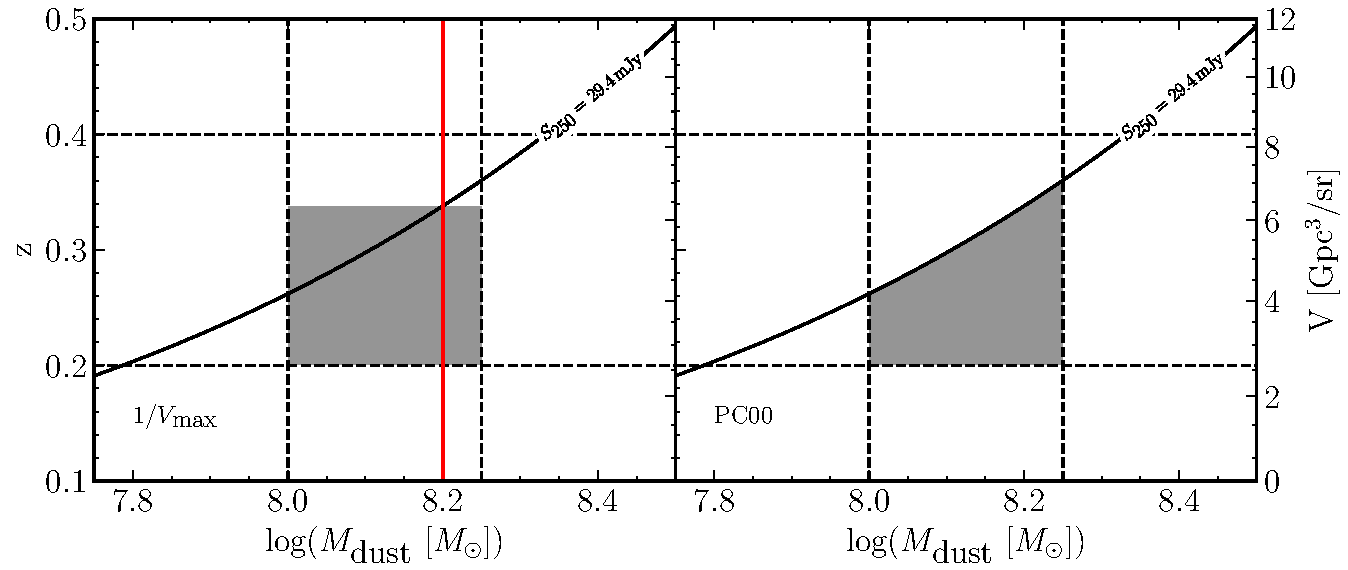
\includegraphics[width=\columnwidth]{Figures/volume_comparison.pdf}
	\caption[Example dust mass - redshift bin for the $1/V_{\textrm{max}}$ and PC00 methods]{An illustration of the accessible volume calculated in the $1/V_{\textrm{max}}$ (left panel) and PC00 methods (right panel), using Equations \ref{eq:volume_1/v_method} and \ref{eq:volume_pc00_method} respectively. Having defined an example dust mass - redshift bin ($8 < \textrm{log}(M_{\textrm{dust}} [M_{\odot}]) < 8.25$, $0.2 < z < 0.4$), the shaded areas in both panels represent the volume - dust mass space that is observable in a \textit{Herschel} survey with a limiting flux of $29.4\,$mJy at $250\,\mu$m. In the $1/V_{\textrm{max}}$ panel we have illustrated the volume as it would appear for an object with a dust mass of $8.2\,\textrm{log}(M_{\odot}$).}
	\label{fig:volume_comparison}
\end{figure}

\section{The Dust Mass Function from Galaxies in the SGP}
\label{sec:dmf_from_sgp}

We apply the three methods described above to the galaxies observed in the H-ATLAS SGP field. It is important to note that our sample is without spectroscopic redshifts and our dust masses are derived from sub-mm fluxes that are susceptible to flux boosting. The resulting scatter in the dust masses and redshifts could move galaxies between neighbouring bins. Given that the volume density is not uniform across bins and the survey is flux-limited, this introduces an Eddington bias (\citealt{Eddington_1913}) that broadens the DMF. For this reason, we model the errors as being formed in two parts. First, a Poissonian error that scales as $\sigma_{\phi,N} \propto \frac{1}{\sqrt{N}}$, where $N$ is the number of galaxies in each bin. The second error term is due to the spread in dust masses as a result of the large uncertainties on our photometric redshifts (see Section \ref{sec:phot_z_VIKING}). When measuring the DMF we run $1000$ Monte Carlo simulations in which we remeasure the DMF having perturbed the redshift of each galaxy according to a Gaussian distribution centered on the assumed redshift and with standard deviation equal to the error value. This gives us a 3D array ($M_{\textrm{dust}} - z - n$, where $n$ is the number of Monte Carlo interations) of $\phi$. We take the standard deviation along the $n$ axis, $\sigma_{\phi,z}^2$, and add this error in quadrature to the Poissonian error: $\sigma_\phi = \sqrt{\sigma_{\phi,N}^2 + \sigma_{\phi,z}^2}$.

Figure \ref{fig:dmf_methods} shows the DMFs derived using the PC00 (solid lines) and $1/V_{\textrm{max}}$ (dashed lines) methods for five redshift bins of width $0.2$, assuming a universal dust temperature of $20\,$K and dust emissivity index, $\beta = 2$. As a single SED shape is being assumed for all galaxies, we must also assume a single survey flux limit - which we take to be $29.4\,$mJy at $250\,\mu$m (\citealt{Valiante_2016}). As we predicted for bins that are entirely above the flux limit of the sample, the two estimators are equivalent. Also predicted earlier was the downturn observed in the lowest dust mass bin in most redshift slices.

The low-mass end of the DMF is typically described by a powerlaw with a slope, $\alpha$, taking values between $-2$ and $-1$. Our DMFs imply a much flatter value, suggesting that the number density of objects between dust masses of $\sim 10^{5.5}\,M_{\odot}$ and $\sim 10^{7.5}\,M_{\odot}$ is near constant. In light of previous H-ATLAS studies that do not predict this behaviour, we expect that this is not a physical trend but rather an indication of an incomplete sample at the lowest masses. Given we are not using spectroscopic redshifts, we are likely missing these galaxies in our sample. From this point onwards we shall assume that our DMFs are accurate above $\sim 10^{7.5}\,M_{\odot}$ and use the results of \citealt{Beeston_2018} to fill in the low-mass regime. We observe a clear evolution in the density of high dust mass galaxies increasing with redshift. The evolution with lookback time is evident in each redshift slice, but noticably slows by the highest redshift bin. This may suggest that there is a point in time at redshifts $\gtrsim 0.8$ where the number density of the most massive galaxies peaks. 

As an extension to our $\phi_{\textrm{est}}$ prediction of the DMF, we would like to be able to use the estimator of \citealt{Dunne_2011} (Equation \ref{eq:phi_pc00_dunne_method}) in which we calculate the acessible volume individually for each source. The problem we face is that this requires knowing the dust temperatures of all galaxies in our sample. While we are able to constrain the dust temperatures for a subset of our sample, as shown in Figure \ref{fig:dust_temperatures}, we cannot depend on these sources alone without introducing another incompleteness to the sample. To avoid this problem we fit a single temperature modified blackbody to all galaxies, with bounds on the cold ISM dust temperature between $15$ and $25\,$K and with a fixed $\beta = 2$. This range of temperatures was chosen as it has been shown to be a suitable range of cold dust temperatures in galaxies (\citealt{Dunne_2001, daCunha_2008, Smith_2012b, Clark_2015, Beeston_2018}). Galaxies that have well constrained peaks in the dust emission are likely to have dust temperatures within this range, and those that have insufficient far-IR data to fit an isothermal model are assumed to take a median value of $20\,$K. Approximately $40\%$ of the galaxies in our sample have temperatures constrained between $15\,$K and $25\,$K; the remaining $\sim 60\%$ retain their $20\,$K assumption. We use this set of dust temperatures to calculate $\phi_{\textrm{est, Dunne}}$ assuming an individual survey flux limit for each source. The flux limit for each galaxy is based on a minimum SNR of four. As pointed out previously in \citealt{Dunne_2011}, this estimator is not equivalent to $\phi_{1/V}$, despite the contribution to $\phi$ being calculated for each galaxy individually in both methods. In the PC00 method we still calculate an average accessible volume for each $M_{\textrm{dust}} - z$ bin, but we now define the limiting dust mass -- redshift relationship for each source based on its own SED. This means we are more precise about the flux limit of the survey but do not depend on the uncertain dust mass estimates of the \textit{Herschel} galaxies. Our estimate of $\phi_{\textrm{est, Dunne}}$ is included in Figure \ref{fig:dmf_methods} (dotted lines). The \citealt{Dunne_2011} estimator of the DMF is broadly consistent with $\phi_{\textrm{est}}$, albeit with a wider distribution of dust masses due to the wider distribution of dust temperatures.

\begin{figure}
	\centering
    \begin{subfigure}{\textwidth}
	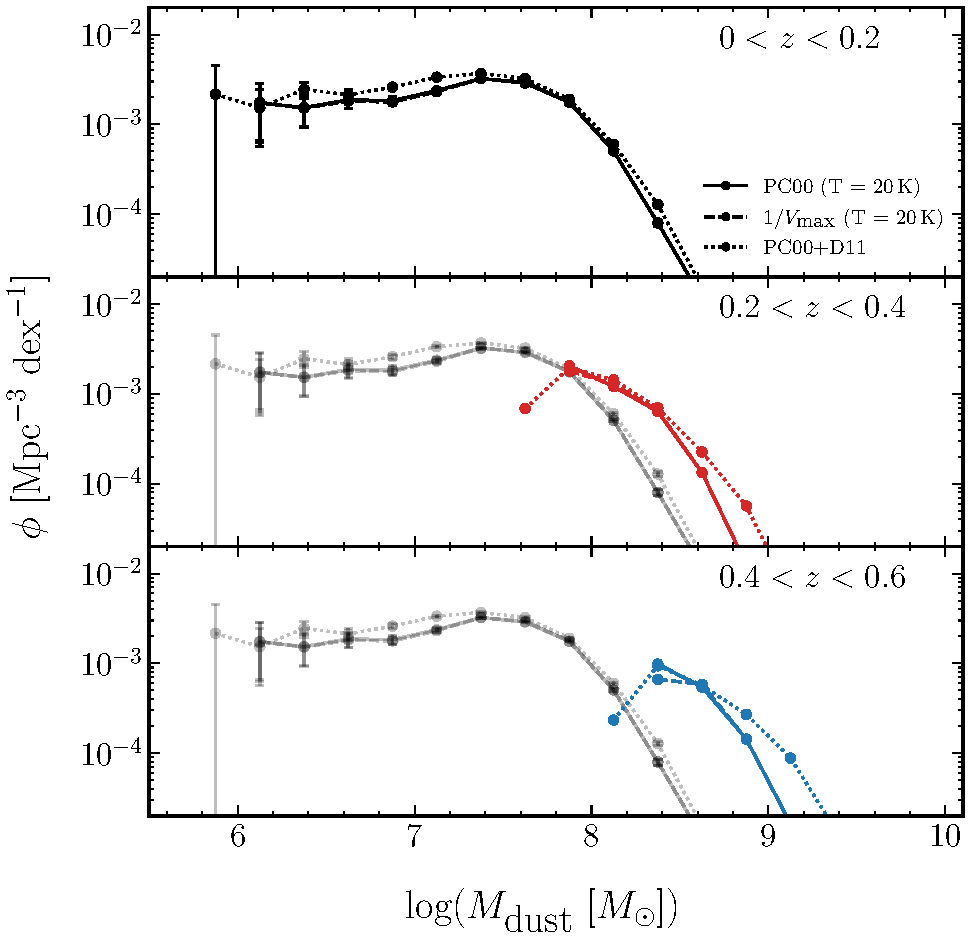
\includegraphics[width=\columnwidth]{Figures/dmf_methods_part1.pdf}
    \end{subfigure}
    \caption[Dust mass functions derived from SGP galaxies]{The dust mass functions (DMFs) derived from SGP galaxies in five redshift bins of width $0.2$. The three methods described in Section \ref{sec:dmf_estimators}; the $1/V_{\textrm{max}}$, the Page and Carrera (\citealt{Page_2000}) and the Page and Carrera with the adaptation from \citealt{Dunne_2011} methods are illustrated as dashed lines, solid lines and dotted lines, respectively. In each panel the DMFs from the first redshift bin are replotted for comparison in grey. The final panel shows the DMFs from all redshift bins.}
	\label{fig:dmf_methods}
\end{figure}

\begin{figure}
    \captionsetup[subfigure]{labelformat=empty}
    \begin{subfigure}{\textwidth}
    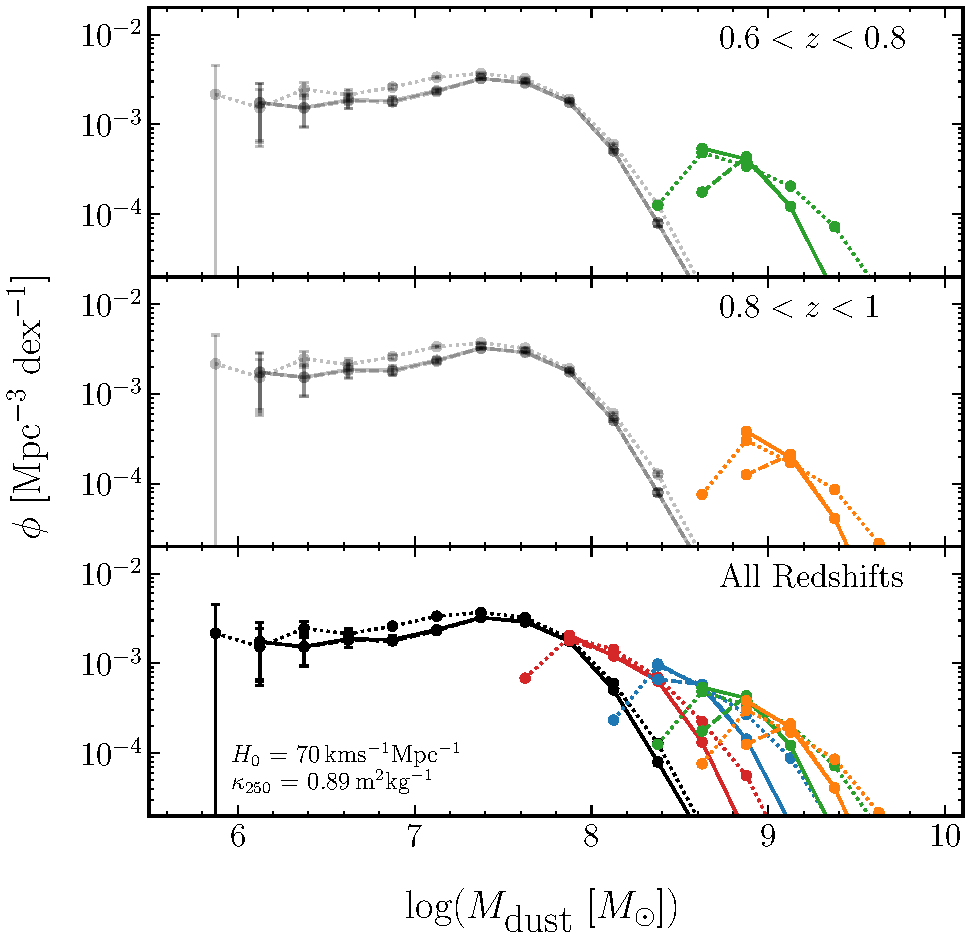
\includegraphics[width=\columnwidth]{Figures/dmf_methods_part2.pdf}
    \subcaption{Continued.}
    \end{subfigure}
\end{figure}

\section{The Evolution in the Dust Content of SGP Galaxies}

In this section, we shall use the results of our two PC00 estimated DMFs to quantify the redshift evolution of dust mass in SGP galaixes. This is achieved in two ways: first by fitting Schechter functions to our DMFs and assessing the evolution in the Schechter parameters, and secondly, by calculating the dust mass density contained within galaxies at different epochs.

\subsection{Schechter Functions}
\label{sec:schechter_functions}

Luminosity functions, and by extension dust mass functions, are often modelled with analytical forms such as broken power laws or Schechter functions. The Schechter function takes the form

\begin{equation}
    \phi(M) dM = \phi^* (M/M^*)^\alpha e^{(-M/M^*)}\frac{dM}{M^*}
    \label{eq:schechter_function}
\end{equation}

\noindent in terms of mass, where $\alpha$ is the slope of the power law at masses below $M^*$; the characteristic dust mass, where we transition from a power law to an exponential tail. The normalization is defined by $\phi^*$ which corresponds to the number density of galaxies at mass $M^*$. We can convert the Schechter function to logarithmic form using the fact that $\phi(\textrm{log}(M)) = \textrm{ln}(10)M\phi(M)$ such that

\begin{equation}
    \phi(\textrm{log}(M)) d\textrm{log}(M) = \textrm{ln}(10)\phi^* e^{-10^{\textrm{log}(M)-\textrm{log}(M^*)}}\times \Bigg(10^{\textrm{log}(M)-\textrm{log}(M^*)}\Bigg)^{\alpha+1} d\textrm{log}(M).
    \label{eq:schechter_function_log}
\end{equation}

We incorporate the factor $\textrm{ln}(10)$ into our definition of $\phi^*$ such that $\phi^*$ has units of Mpc$^{-3}$dex$^{-1}$. Given the incompleteness of the lowest mass bins at high redshifts, it is common to fit the three Schechter parameters ($\phi^*$, $M^*$ and $\alpha$) for the first redshift bin and make the assumption that the value of $\alpha$ does not vary with redshift. Due to our sample incompleteness at low dust masses even in the lowest redshift slice, we fix our value of $\alpha$ to the \citealt{Beeston_2018} value of $-1.22$ throughout, and only consider values greater than $10^{7.5}\,M_{\textrm{dust}}$ in our fitting.

Figure \ref{fig:dmf_schechter} shows the best fit Schechter functions to our $\phi_{\textrm{est}}$ (solid lines, filled circles) and $\phi_{\textrm{est, Dunne}}$ (dotted lines, open circles) DMFs. The fitting parameters are listed in Table \ref{tab:schechter_parameters}. Included in Figure \ref{fig:dmf_schechter} are the studies of \citealt{Vlahakis_2005}, \citealt{Dunne_2011}, \citealt{Beeston_2018} and \citealt{Pozzi_2020}. For a direct comparison between all works we have scaled the DMFs in the literature to the same cosmology ($\Omega_m = 0.3$, $\Omega_\Lambda = 0.7$ and $H_0 = 70\,$km s$^{-1}$Mpc$^{-1}$) and dust mass absorption coefficient ($\kappa_{250} = 0.89\,$m$^{2}$kg$^{-1}$).

\begin{figure}
	\centering
    \begin{subfigure}{\textwidth}
	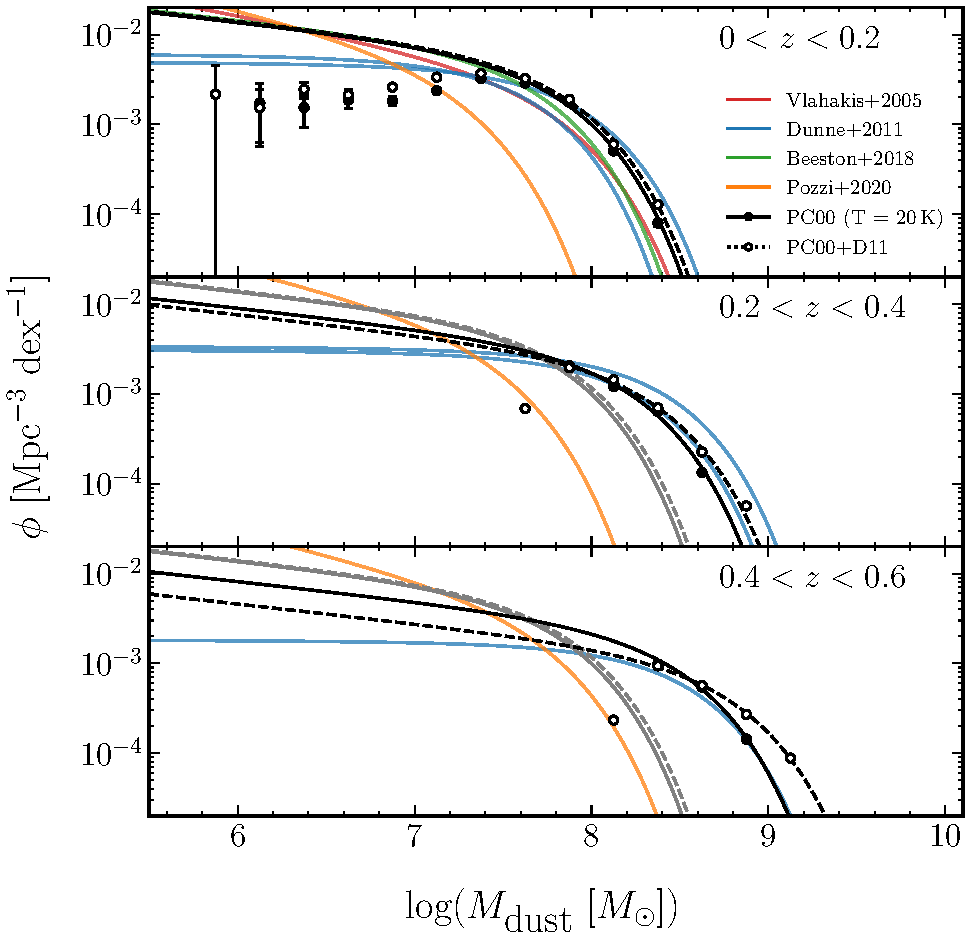
\includegraphics[width=\columnwidth]{Figures/dmf_schechter_part1.pdf}
    \end{subfigure}
    \caption[Schechter functions derived from the SGP DMFs alongside relevant studies]{The dust mass functions as presented in Figure \ref{fig:dmf_methods} (excluding the $1/V_{\textrm{max}}$ estimate), where the lines have been replaced with the best fitting Schechter functions (Equation \ref{eq:schechter_function_log}). The red, blue, green and orange lines represent the DMFs from \citealt{Vlahakis_2005}, \citealt{Dunne_2011}, \citealt{Beeston_2018} and \citealt{Pozzi_2020} respectively. The final panel shows the SGP DMFs from all redshift bins. The colour scales from the light to dark with increasing redshift.}
	\label{fig:dmf_schechter}
\end{figure}

\begin{figure}
    \captionsetup[subfigure]{labelformat=empty}
    \begin{subfigure}{\textwidth}
    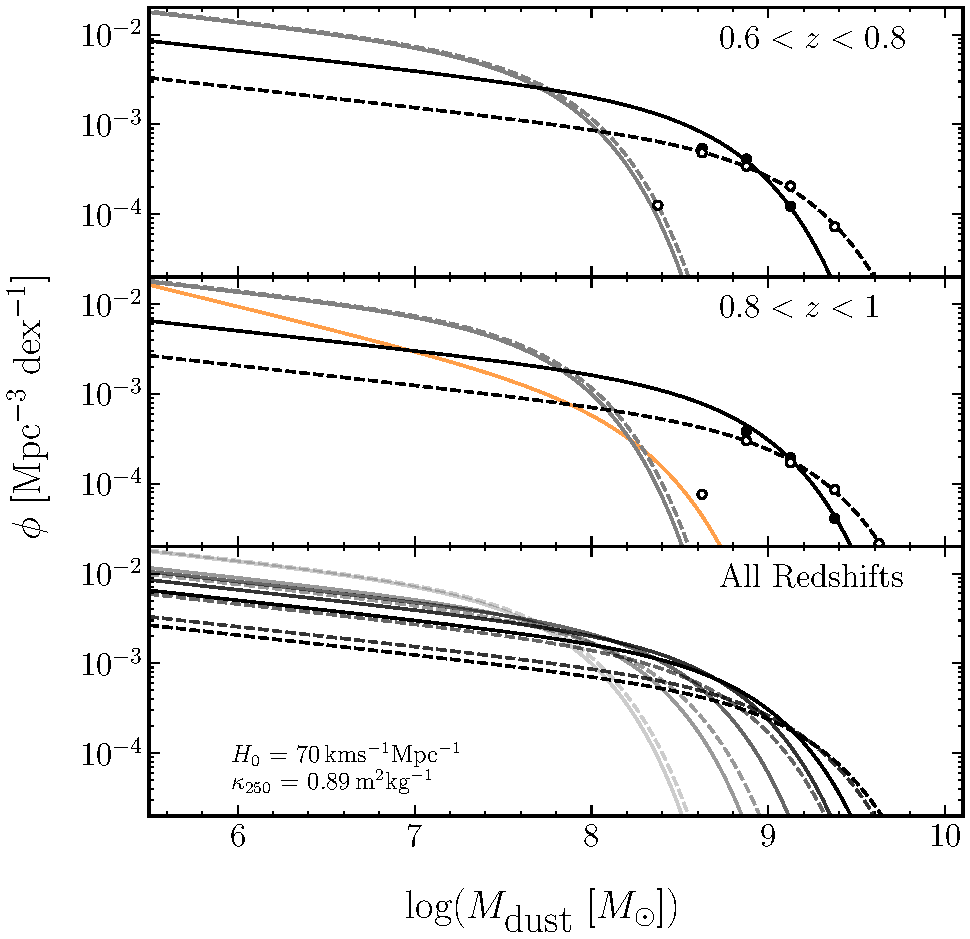
\includegraphics[width=\columnwidth]{Figures/dmf_schechter_part2.pdf}
    \subcaption{Continued.}
    \end{subfigure}
\end{figure}


\begin{table}
    \centering
    \begin{tabular}{p{1.75cm}|p{2.5cm}|p{2cm}|p{3.25cm}|p{1.25cm}|p{2cm}}
        \hline
        \hline
        Method & Redshift & log($M_{\textrm{dust}}^*$) & log($\phi^*$) & $\alpha$ & $\rho_{\textrm{dust}} (\times10^5)$ \\
        & & [log($M_{\odot}$)] & [log(Mpc$^{-3}$dex$^{-1}$)] & & [$M_{\odot}$Mpc$^{-3}$] \\
        \hline
        \hline
        \multirow{5}{*}{$\phi_{\textrm{est}}$} & 0 < z < 0.2 & $7.791^{+0.007}_{-0.007}$ & $-2.256^{+0.010}_{-0.011}$ & $-1.22$ & $1.770^{+0.051}_{-0.050}$ \\
        & 0.2 < z < 0.4 & $8.183^{+0.004}_{-0.005}$ & $-2.528^{+0.008}_{-0.008}$ & $-1.22$ & $2.331^{+0.048}_{-0.048}$ \\
        & 0.4 < z < 0.6 & $8.468^{+0.005}_{-0.005}$ & $-2.629^{+0.010}_{-0.010}$ & $-1.22$ & $3.560^{+0.088}_{-0.087}$ \\
        & 0.6 < z < 0.8 & $8.745^{+0.004}_{-0.004}$ & $-2.801^{+0.009}_{-0.009}$ & $-1.22$ & $4.542^{+0.104}_{-0.101}$ \\
        & 0.8 < z < 1 & $8.890^{+0.005}_{-0.005}$ & $-2.930^{+0.012}_{-0.012}$ & $-1.22$ & $4.695^{+0.139}_{-0.136}$ \\
        \hline
        \multirow{5}{*}{$\phi_{\textrm{est, Dunne}}$} & 0 < z < 0.2 & $7.827^{+0.007}_{-0.007}$ & $-2.249^{+0.010}_{-0.010}$ & $-1.22$ & $1.952^{+0.054}_{-0.053}$ \\
        & 0.2 < z < 0.4 & $8.305^{+0.004}_{-0.004}$ & $-2.628^{+0.006}_{-0.006}$ & $-1.22$ & $2.451^{+0.041}_{-0.040}$ \\
        & 0.4 < z < 0.6 & $8.747^{+0.005}_{-0.005}$ & $-2.943^{+0.006}_{-0.006}$ & $-1.22$ & $3.288^{+0.059}_{-0.059}$ \\
        & 0.6 < z < 0.8 & $9.117^{+0.003}_{-0.003}$ & $-3.277^{+0.003}_{-0.003}$ & $-1.22$ & $3.570^{+0.039}_{-0.039}$ \\
        & 0.8 < z < 1 & $9.195^{+0.004}_{-0.004}$ & $-3.386^{+0.004}_{-0.004}$ & $-1.22$ & $3.323^{+0.044}_{-0.044}$ \\
        \hline
    \end{tabular}
    \caption[Best fitting Schechter parameters of our SGP DMFs in each redshift slice]{The best fitting Schechter parameters for each redshift slice. The parameter $\phi^*$ incorporates the factor \textrm{ln}(10) such that it has units of Mpc$^{-3}$dex$^{-1}$. The uncertainties in the Schechter parameters are taken from the $16$th to $84$th percentiles of the posterior distribution for each parameter. The rightmost column lists the dust mass densities as calculated using Equation \ref{eq:dust_mass_density}.}
    \label{tab:schechter_parameters}
\end{table}

The local DMFs ($z < 0.2$) are in good agreement except for the low-mass normalization found by \citealt{Dunne_2011} and the offset in dust mass with the study of \citealt{Pozzi_2020}. While it is hard to reconcile the low normalization of the \citealt{Dunne_2011} DMF with other works in the literature without a full understanding of the completeness of the respective samples at low flux densities, the shift in dust mass observed by \citealt{Pozzi_2020} in all redshift bins can be understood by comparing the selection wavelengths of the samples and their sensitivity to dust temperature. As mentioned previously, estimating dust masses from long wavelength photometry is advantageous as the Rayleigh-Jeans (R-J) part of the Planck function is least sensitive to dust temperature and most sensitive to dust mass. In the R-J regime ($\lambda_{\textrm{rest}} \gg \frac{hc}{kT}$) the Planck function reduces to $B(\nu_{250}, T) = \frac{2\nu_{250}^{2}kT}{c^2}$ which means that in the optically thin and R-J regimes our dust masses are only linearly dependent on the dust temperature.

This work, as well as the studies of \citealt{Dunne_2011} and \citealt{Beeston_2018}, are based on samples of H-ATLAS sources which are primarily selected at $250\,\mu$m. In the rest frame of the highest redshift galaxies considered here, the selection wavelength is still expected to be on the long wavelength side of the peak in thermal dust emission. Further, at $850\,\mu$m, the SLUGS study of \citealt{Vlahakis_2005} is securely on the R-J side of the SED at the low redshifts probed in the SCUBA-selected study. As a result, these studies are sensitive to thermal emission from dust with fairly cool temperatures which should probe most of the dust mass. The $160\,\mu$m selection wavelength of \citealt{Pozzi_2020} means that in the rest frame this study probes different parts of the dust spectrum, crossing the peak to shorter wavelengths at $z \sim 0.5$. As we approach the peak of the dust SED an estimate of the dust mass becomes increasingly dependent on the measurement of the dust temperature - an effect that should also be noted when making conclusions from the highest redshift bins in our study. This is not to say that any study is inaccurate, but rather suggests that comparing studies with samples selected at different wavelengths may differ significantly, particularly if their dust temperatures are very different. It is also worth pointing out that there is a clear offset from the \citealt{Pozzi_2020} DMF even at $0 < z < 0.2$, where this effect is the least impactful, and therefore is not explained by this argument.

\subsection{Evolution of the Dust Mass Function}

To quantify the evolution we observe in dust masses of SGP galaxies, we can illustrate the variation in the characteristic dust mass and density in each redshift slice as obtained from our best fitting Schechter functions. Figure \ref{fig:dmf_schechter_parameters} shows the distribution of $\phi^*$ and $M_{\textrm{dust}}^*$ for our $\phi_{\textrm{est}}$ and $\phi_{\textrm{est, Dunne}}$ DMFs, as well as the studies considered in Figure \ref{fig:dmf_schechter}. We observe a strong evolution in the characteristic dust mass $M_{\textrm{dust}}^*$ with redshift, suggesting that galaxies were dustier at higher redshift. The density $\phi^*$ appears to decrease with redshift, but this is dependent on how well we account for the incompleteness in the sample and is known to be degenerate with $M_{\textrm{dust}}^*$. The characteristic dust mass evolves from $M_{\textrm{dust}}^* = 6.18\times10^7\,M_{\odot}$ at $z < 0.2$ to $M_{\textrm{dust}}^* = 7.76\times10^8\,M_{\odot}$ at $z = 0.8 - 1$, assuming a universal dust temperature of $20\,$K, suggesting a factor of $\sim 13$ in dust mass between the highest and lowest redshift bins. If we allow the $\sim 40\%$ of galaxies with well constrained dust temperatures to define their own K-corrections, then we observe a much steeper evolution from $M_{\textrm{dust}}^* = 6.71\times10^7\,M_{\odot}$ to $M_{\textrm{dust}}^* = 1.57\times10^9\,M_{\odot}$ over the same time period. This implies a factor increase twice as large compared to our $T_{\textrm{dust}} = 20\,$K DMF.

\begin{figure}
	\centering
	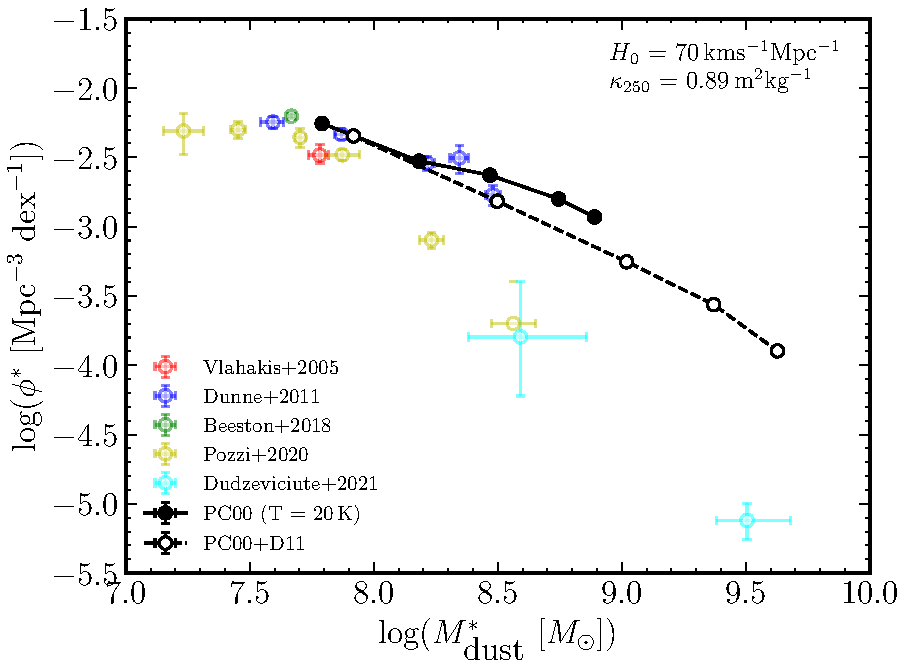
\includegraphics[width=0.8\columnwidth]{Figures/dmf_schechter_parameters.pdf}
	\caption[Distribution of $M_{\textrm{dust}}^*$ and $\phi^*$ from best fitting Schechter functions]{The distribution of $M_{\textrm{dust}}^*$ and $\phi^*$ for the two estimates of the DMF considered in this study ($T = 20\,$K shown as filled circles with solid lines and the \citealt{Dunne_2011} adaptation shown as open circles with dotted lines). The studies from the literature are the same as those given in Figure \ref{fig:dmf_schechter}.}
	\label{fig:dmf_schechter_parameters}
\end{figure}

Figure \ref{fig:dmf_m_evolution} shows the variation in the characteristic dust mass as a function of redshift. We fit the observed relationships with a function of the form $\textrm{log}(M_{\textrm{dust}}^*) = \textrm{log}(M_{\textrm{dust,0}}^*)(1+z)^\gamma$. The best fitting functions are given by $\textrm{log}(M_{\textrm{dust}}^*) = (7.66\pm0.10)(1+z)^{0.30\pm0.03}$ when dust temperature is allowed to be free between $15$ and $25\,$K, and $\textrm{log}(M_{\textrm{dust}}^*) = (7.65\pm0.05)(1+z)^{0.24\pm0.01}$ when assuming $T_{\textrm{dust}} = 20\,$K. The $\textrm{log}(M_{\textrm{dust,0}})$ term represents a typical galaxy's dust mass at redshift zero, which is in excellent agreement between the two models. Using these fitted relationships we find that at $z = 1$, the galaxies detected by \textit{Herschel} were typically $60$ times dustier (or $\sim 25$ times when assuming $T_{\textrm{dust}} = 20\,$K) approximately $8\,$Gyr ago. \citealt{Dunne_2011} found that the most massive galaxies at the highest redshifts probed in their study, $z \sim 0.5$, have dust masses a factor of $5$ to $8$ larger than those at $z \sim 0$. At the same redshift, our empirical relationships find that the characteristic dust mass evolves by a factor of $6 - 10$, in good agreement with \citealt{Dunne_2011}.

\begin{figure}
	\centering
	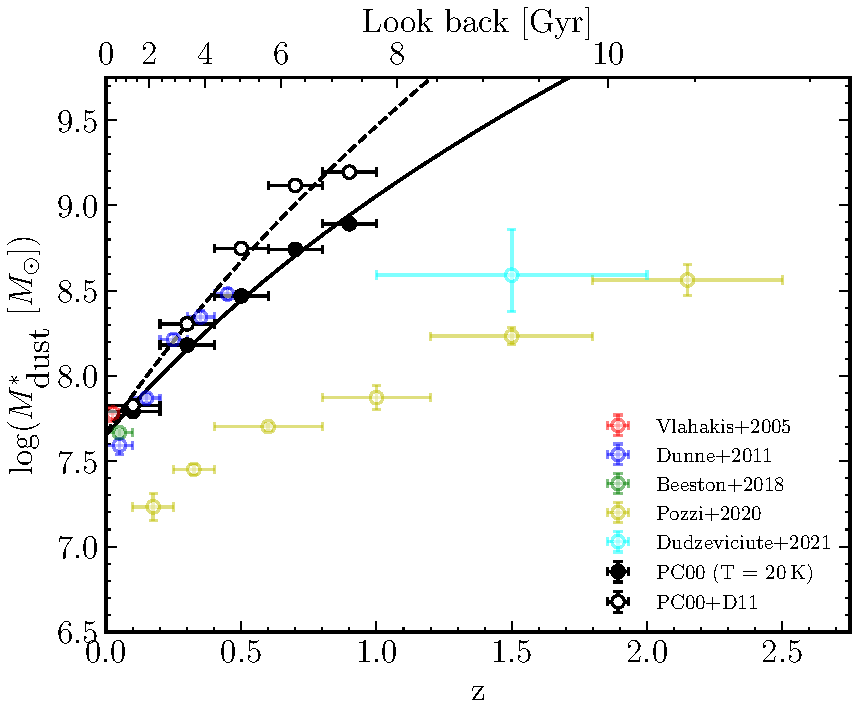
\includegraphics[width=0.8\columnwidth]{Figures/dmf_m_evolution.pdf}
	\caption[Evolution of the characteristic dust mass, $M_\textrm{dust}^*$, as a function of redshift]{The best fitting characteristic dust mass, $M_\textrm{dust}^*$, as a function of redshift. The coloured error bars have the same colour convention as Figure \ref{fig:dmf_schechter}. The solid and dotted lines represent best fitting relationships of the form $\textrm{log}(M_{\textrm{dust,0}}^*)(1+z)^\gamma$. For our $T_{\textrm{dust}} = 20\,$K DMF we find $\gamma = 0.24\pm0.01$ and $\gamma = 0.30\pm0.03$ when temperature is allowed to be free between $15\,$K and $25\,$K.}
	\label{fig:dmf_m_evolution}
\end{figure}

\subsection{Dust Mass Density}

As the Schechter parameters are correlated, more meaningful estimators of the dust content of galaxies across cosmic time are the integrated dust mass density (DMD), $\rho_{\textrm{dust}}$, and the dust mass density parameter, $\Omega_{\textrm{dust}}$. We integrate the DMFs in each redshift slice to calculate the total amount of dust in galaxies at different epochs. This integration is given by

\begin{equation}
    \rho_{\textrm{dust}} = \int_0^\infty M_{\textrm{dust}} \phi(M_{\textrm{dust}}) dM_{\textrm{dust}} = \Gamma(2+\alpha) M_{\textrm{dust}}^* \phi^*,
    \label{eq:dust_mass_density}
\end{equation}

\noindent where $\Gamma(x)$ represents the Gamma function, $\Gamma(x) = \int_0^\infty t^{x-1}e^{-t} dt$, and $\phi(M_{\textrm{dust}})$ has been substituted with the best fitting Schechter function. The dust mass density measured in this way is built upon a number of assumptions. First, it is assumed that the Schechter function is applicable at dust masses far below the range that has been directly measured. We could circumvent this problem by integrating to some common lower mass limit using the upper incomplete Gamma function, $\Gamma(x, z) = \int_z^\infty t^{x-1}e^{-t} dt$, however, all the studies considered here have varying levels of completeness at low masses and the integrated density without imposing this limit is negligibly different. As such, the DMD calculated using Equation \ref{eq:dust_mass_density} serves as a maximal estimate of the dust mass density. Second, the low mass slope is assumed to be constant with redshift such that the number density of lower mass galaxies does not change with time. This assumption has no motivation, but is not expected to have a significant impact on our dust mass densities as the majority of the contribution by mass comes from the much fewer, more massive galaxies. The dust mass density parameter is obtained from $\Omega_{\textrm{dust}} = \rho_{\textrm{dust}}/\rho_{\textrm{crit}}$ where $\rho_{\textrm{crit}} = 1.36\times10^{11}\,M_{\odot}$Mpc$^{-3}$ is the critical density for our assumed cosmology. The dust densities are listed in Table \ref{tab:schechter_parameters} and shown in Figure \ref{fig:dmd} alongside the measured values for the studies previously mentioned. 

\begin{figure}
	\centering
	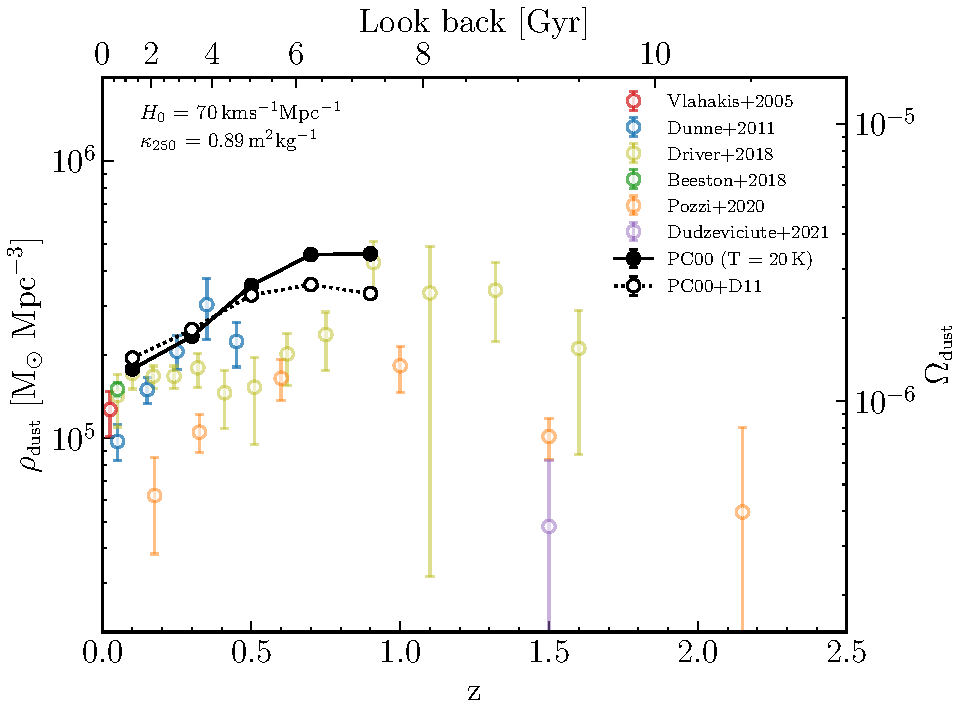
\includegraphics[width=0.8\columnwidth]{Figures/dmd.pdf}
	\caption[Integrated dust mass density as a function of redshift]{The integrated dust mass density and dust density parameter as a function of redshift for SGP galaxies, calculated using Equation \ref{eq:dust_mass_density}. The coloured error bars have the same colour convention as Figure \ref{fig:dmf_schechter}, with the addition of the study of \citealt{Driver_2018} (light green).}
	\label{fig:dmd}
\end{figure}

In reasonable agreement with \citealt{Dunne_2011}, we predict a rapid evolution in dust mass density in the local universe, though it is notably less steep than the $(1+z)^{4.5}$ relationship observed in their study. Our measurement of the dust mass density suggests a factor $\sim 1.7 - 2.6$ increase between $0 < z < 0.2$ and $0.8 < z < 1$, beyond which the dust density remains roughly constant, suggesting a peak at redshifts around $0.8 - 1$. The rapid decrease in dust density from $z \sim 1$ to the present day may have a number of possible causes. First, the depletion of dust due to star formation, owing to the fact that evolution in dust mass and SFR are intrinsically related since stars form out of gas and the dust is expected to trace the interstellar gas reservoir. The decline may also be attributed to dust destruction or dust lost from the galaxy to the halo (\citealt{Dunne_2011}). In contrast to the prevailing \textit{Herschel} view, \citealt{Driver_2018} find a relatively flat density at redshifts $< 0.5$, though it is noted that the method used to calculate the incompleteness in their sample differs from the one used here, and by extension in \citealt{Dunne_2011}, which may be the root cause of the difference.

The prediction of a peak in the dust density varies among studies. \citealt{Driver_2018} study the stellar mass and dust mass density of GAMA sources out to redshift five, and thus probe a large span of cosmic time in order to locate a peak in the dust density at $z \sim 1$. Our two DMFs predict a similarly timed peak in the dust density at $z \sim 0.8 - 1$. In contrast, the dust mass density described by \citealt{Dunne_2011} appears to drop in the last redshift bin ($0.4 < z < 0.5$) despite an increase in the characteristic dust mass, suggesting a peak at much later cosmic times. However, the significance of this result is doubtful as this drop in density could be attributed to incompleteness or a photometric redshift bias resulting from the lack of spectroscopic redshifts in this bin. In our study we only use photometric redshifts, but have factored the additional uncerainty this creates in our DMFs by running Monte Carlo simulations (Section \ref{sec:dmf_from_sgp}). We find that the contribution to the error budget from using photometric redshifts is of order the Poissonian errors and do not have a significant effect on the Schechter fitting and resulting dust mass densities. If, however, there were a systematic trend in the photometric redshifts, we might expect the observed evolution to change in steepness and/or shift the apparent peak to different redshifts.

\subsection{Comparison with the Star Formation Rate Density}

There is a direct link between star formation and the dust and gas content of galaxies. The Kennicutt-Schmidt relationship demonstrates the link between the gas and star formation rate surface densities of galaxies. Given that dust traces the gas in the ISM, there is a consequential link between dust content and the star formation activity. As a result, it is constructive to look at the dust mass density we observe from the galaxies in the SGP with the mean star formation rate in the Universe.

The redshift dependence of the cosmic star formation history given by \citealt{Madau_2014}, which takes the form of a double power law in $(1 + z)$, is based on the best fit to multiple UV and IR data sets representing the unobscured and obscured star formation densities. Combining these surveys provides a clear and comprehensive picture of the cosmic star formation activity. The best fitting function is given by

\begin{equation}
    \psi(z) = 0.015\frac{(1+z)^{2.7}}{1+[(1+z)/2.9]^{5.6}} [M_{\odot}\textrm{yr}^{-1}\textrm{Mpc}^{-3}].
    \label{eq:madau_sfrd}
\end{equation}

This expression implies a cosmic star formation history that scales as $(1+z)^{-2.9}$ between $3 \lesssim z \lesssim 8$, a peak in the range $1.5 \lesssim z \lesssim 2$, and a decline of the form $(1+z)^{2.7}$ to the present day. Figure \ref{fig:sfrd} shows our measurements of the dust mass density alongside the measurements of the mean star formation rate in the Universe. The offset between the two scales has been set to follow the relationship $\rho_{\textrm{dust}} = \rho_{\textrm{gas}}/\delta_{\textrm{gdr}} \sim \psi \times\tau_{\textrm{depl}}/\delta_{\textrm{gdr}}$, where we have assumed a typical depletion timescale, $\tau_{\textrm{depl}}$, of $500\,$Myr and a gas mass to dust mass ratio, $\delta_{\textrm{gdr}}$, of $100$. However, we do not intend for this to be interpreted as a suitable definition for the star formation density of SGP galaxies, rather as an approximation such that the two sets of measurements roughly coincide. 

\begin{figure}
	\centering
	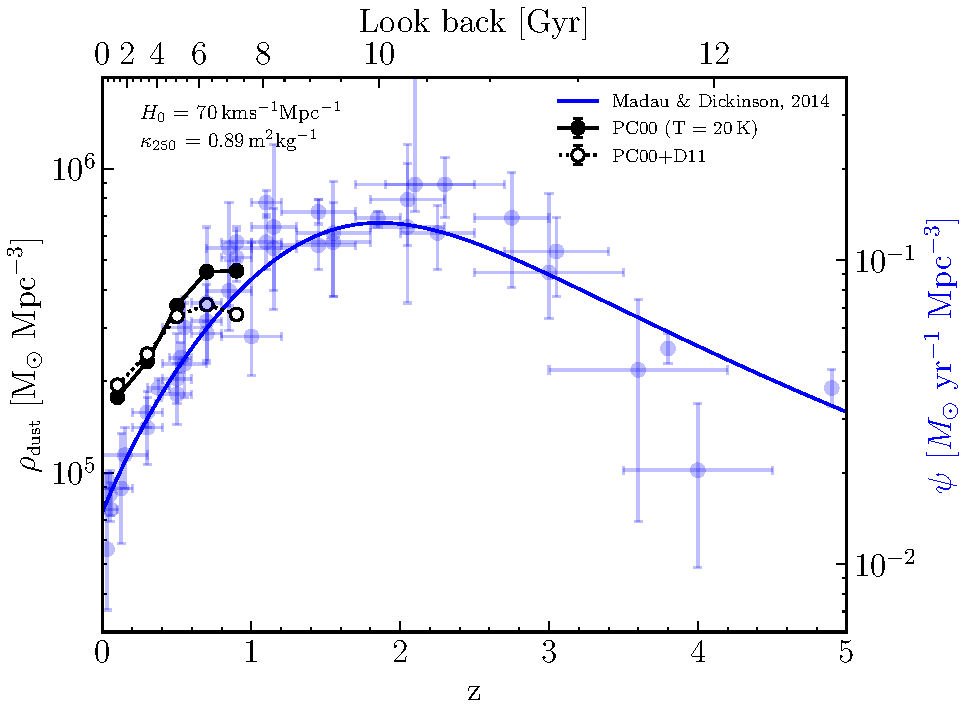
\includegraphics[width=0.8\columnwidth]{Figures/sfrd.pdf}
	\caption[Comparison of dust mass density and the cosmic star formation rate density]{The integrated dust density of SGP galaxies as illustrated in Figure \ref{fig:dmd}. The blue error bars represent the various studies included in the fitting of \citealt{Madau_2014} for the cosmic star formation rate density (blue line). The two vertical axes have been scaled for illustrative purposes using $\rho_{\textrm{dust}} \sim \psi \times\tau_{\textrm{depl}}/\delta_{\textrm{gdr}}$, where we have assumed a typical depletion timescale of $500\,$Myr and a gas mass to dust mass ratio of $100$. The studies used in the measurement of the SFRD include: \citealt{Sanders_2003}, \citealt{Takeuchi_2003}, \citealt{Wyder_2005}, \citealt{Schiminovich_2005}, \citealt{Reddy_2009}, \citealt{Robotham_2011}, \citealt{Magnelli_2011}, \citealt{Cucciati_2012}, \citealt{Bouwens_2012b}, \citealt{Bouwens_2012a}, \citealt{Schenker_2013}, \citealt{Magnelli_2013}, \citealt{Gruppioni_2013} and \citealt{Dahlen_2007}.}
    \label{fig:sfrd}
\end{figure}

The similarity in the evolutions of the dust mass density and the star formation rate density (SFRD) to the present day show that the two are intrinsically linked, and that the quantity of dust contained in galaxies is dependent on recent star formation. We know that dust can be formed in several ways: the stellar winds of evolved asymptotic giant branch (AGB) and red giant branch (RGB) stars, supernovae and grain growth in the ISM. These dust production mechanisms have appreciably different timescales, the shortest being from the stellar sources. The short timescale ($\sim 2 - 3\,$Gyr) between the peak in the SFRD predicted by \citealt{Madau_2014} and the peak in the dust mass density measured by our DMFs (though we add the caveat that this is highly dependent on our highest redshift bin, which may be subject to biases in photometric redshifts) gives credit to the idea that stellar sources form a substantial contribution to dust production. 

\section{Conclusion}

In this Chapter, we derived the dust masses of our SGP galaxies assuming an isothermal modified blackbody, setting limits on the temperature of the cold dust reservoir between $15$ and $25\,$K. From our sample we derived binned dust mass functions in redshift slices out to $z = 1$, representing approximately $8$ billion years in the past. We explored the differences between two measures of the DMF; one in which the cold dust is assumed to be constant at $20\,$K for all galaxies, and one where the dust temperature was allowed to vary within the predetermined bounds. The two methods yield similar results and are presented together without preference. From the evolution in the characteristic dust mass, we estimated that \textit{Herschel} detected galaxies were on average $25$ to $60$ times dustier at $z = 1$ than they are today. Next, we integrated both DMFs for the total amount of dust in \textit{Herschel} galaxies at various points in time. This dust mass density showed a rapid evolution from $z = 1$ to $z = 0$ of a factor approximately half, suggesting significant dust depletion due to star formation, dust destruction or dust lost to the halo over the past $8\,$Gyr. There is tentative evidence of a peak in the dust mass density at redshifts between $0.8$ and $1$, which if true, would lag no more than $2 - 3\,$Gyr behind the peak in the star formation rate density at $z \sim 2$. This implies a strong contribution from stellar sources of interstellar dust, which typically have shorter production timescales. 



\chapter{Dust Properties of IR-bright, Star Forming Galaxies}
\label{chapter:Dust_Evolution}
\section{Introduction}

[In the previous chapter (DMFs) I show the evolution in dust masses assuming Galactic dust at all redshifts (i.e T=20K and beta=2), this chapter will tackle this assumption.]

\section{Dust Properties of DSFGs}

Interstellar dust plays a crucial role in the formation of galaxies as dust grains are the site of molecule formation like molecular hydrogen, $H_2$, the primary fuel for star formation (\citealt{Kennicutt_2012}). $H_2$ is the most abundant molecule in the Universe but is difficult to observe directly unless originating from energetic environments. Alternatives include observing less abundant molecules such as CO and using conversion factors to estimate the mass of molecular hydrogen, or observing dust emission to estimate dust masses (as in the previous chapter) and assuming gas-to-dust ratios (e.g. \citealt{Saintonge_2013}) to convert these into estimates for the total gas mass in high-redshift galaxies (e.g. \citealt{Magdis_2012}; \citealt{Eales_2012}; \citealt{Scoville_2014}; \citealt{Santini_2014}; \citealt{Genzel_2015}). Such studies have shown that galaxies at high redshift contain a higher fraction of gas than galaxies today (\citealt{Tacconi_2010}; \citealt{Scoville_2016}; \citealt{Scoville_2017}; \citealt{Millard_2020}), showing that direct observations of dust emission are useful in our understanding of how galaxies grow and evolve. It is important to note, however, that studies that make these links between dust emission and the evolution of galactic properties make the basic assumption that properties of the dust remain constant with redshift. In the following we investigate the possibility of evolution in dust itself by modelling the dust emission from a sample of high-redshift galaxies and measuring their dust properties over a large expanse of cosmic history.

Of particular importance to us is the dust emissivity spectral index, $\beta$, which controls the frequency dependence of the emissivity of dust grains per unit mass. By assuming, as is customary, that the optical depth of a galaxy can be approximated as a power law of the form $\tau \propto \nu^\beta$, we are implicity assuming that $\beta$ encodes within it information about the dust grain properties such as their chemical composition and their size and growth. The assumed value of $\beta$ for a galaxy can have significant consequences on the assumed absorption properties of the dust grains and consequently on fundamental properties of the ISM in the galaxy such as the total mass of dust (\citealt{Bianchi_2013}; \citealt{Clark_2016}).

Theoretical models for dust (e.g. \citealt{Draine_1984}; \citealt{Draine_2011}; \citealt{Kohler_2015}) predict $\beta$ values to range between approximately 1 -- 2 depending on the chemical composition of the dust grains. Adopting suitable fixed values of $\beta$ have been vital for estimates of the dust temperature and dust luminosity of galaxies in past studies, particularly for high-redshift sources that often lack constraints in the far-infrared (e.g. \todo[color=green]{Add references}). A nominal value of $\beta$ = 2 is common practice in this scenario as it mimics the emissivity of mixtures of amorphous silicates and graphites that well represent the optical properties of Galactic dust grains. However, recent studies have shown that the value of $\beta$ can take a wide variety of values among local galaxies and even among different regions within the same galaxy. For example, \citealt{Lamperti_2019} model the far-infrared dust SEDs of 192 nearby galaxies from the JCMT dust and gas In Nearby Galaxies Legacy Exploration (JINGLE) survey and observed a range of temperatures for the cold dust between 17 and 30\,K and dust emissivity spectral indices between 0.6 and 2.2. Within M31 (Andromeda) \citealt{Smith_2012}, \citealt{Draine_2014} and \citealt{Whitworth_2019} identified a decrease in $\beta$ with galactocentric radius, potentially a result of $\beta$ evolving to higher values when observed in denser regions of the ISM due to grain coagulation. A follow up study by \citealt{Athikkat-Eknath_2022} compared the average $\beta$ measured inside and outside molecular clouds within M31, and while there was no evidence to support the idea that $\beta$ varies due to dense molecular gas, the radial variation in $\beta$ remained present. At higher redshifts, where the far-infrared part of the spectrum is spatially unresolved, it is not possible to constrain the true value of a galaxy's $\beta$ but can be used to define an \textit{effective} $\beta$ value that represents the integrated dust properties over the whole galaxy. [...]\todo[color=orange]{Importance of having an effective $\beta$ value.}

\section{Obtaining Redshifts from Carbon Monoxide Lines}

In order to study the evolution of the dust properties of DSFGs we require robust redshifts to place their formation in cosmic history and to determine accurate measurements of fundamental properties. Obtaining robust ages of galaxies in the form of spectroscopically determined redshifts is hampered by the poor spatial resolution of single-dish observations, which worsens with increasing redshift. While DSFGs can be discovered at far-infrared and sub-mm wavelengths to high redshifts directly from the photometry of the sub-mm source, selecting those with distinctly red sub-mm colours in the \textit{Herschel} bands (e.g. \citealt{Dowell_2014}; \citealt{Ivison_2016}; \citealt{Donevski_2018}; \citealt{Duivenvoorden_2018}), careful consideration of the selection wavelength is required to make optimal use of the negative K-correction. For example, the \textit{Herschel}-SPIRE bands increasingly probe the peak of the dust SED at higher redshifts, making them less sensitive to unlensed DSFGs beyond z $\sim$ 2 -- 3. Additionally, the dust-obscured nature of this population of galaxies makes the identification of counterparts at other wavelengths where spectroscopically determined reshifts are readily available more difficult, which is compounded by the poor resolution and source confusion in the sub-mm (see the Likelihood Ratio analysis of Chapter \ref{chapter:Data_Release_3} for an example).

A more reliable method for robust redshifts is to follow up single-dish observations with inteferometric measurements with interferometers such as the Atacama Large Millimeter/submillimeter Array (ALMA). An even more direct way of obtaining redshfits while observing sources in the sub-mm/mm wavebands is to observe molecular emission lines which can be directly associated with the sub-mm emission without the need for intermediary steps with high-resolution imaging. Recent advancements in the possible bandwidths of instruments like ALMA and the Northern Extended Millimetre Array (NOEMA) have allowed for the ability to detect spectral lines (typically from CO or [CII]) that emanate unambiguously from the sub-mm source. CO is the second most abundant molecule in the Universe after $H_2$ and has rotational transitions that produce some of the brightest lines in the millimeter spectrum. The brightness of the CO lines result from the abundance of CO, the low excitation energy of the transitions and the wavelengths at which they occur coinciding with regions of the spectrum with high atmospheric transmission probed by ALMA. A secondary advantage of using molecular emission to determine spectroscopic redshifts is that they are independent of the photometry used to describe the dust SED and are therefore less prone to bias. In Figure \ref{fig:redshift_ladder} I show the coverage of CO line transitions as functions of the redshift and observed wavelength. We see that at [...] wavelengths, there is a non-uniform coverage of CO transitions, meaning that sources believed to be at a particular redshift may have multiple line detections, allowing for unambiguous constraints on the redshift of the galaxy, single line detections, which allows for some abiguity to the redshift solution, or no line detections. In the regions where no CO lines can be detected by a particular instrument, "redshift deserts" appear as breaks in the redshift distribution of galaxies.

\todo[color=red]{Complete figure and add caption}
\begin{figure}
	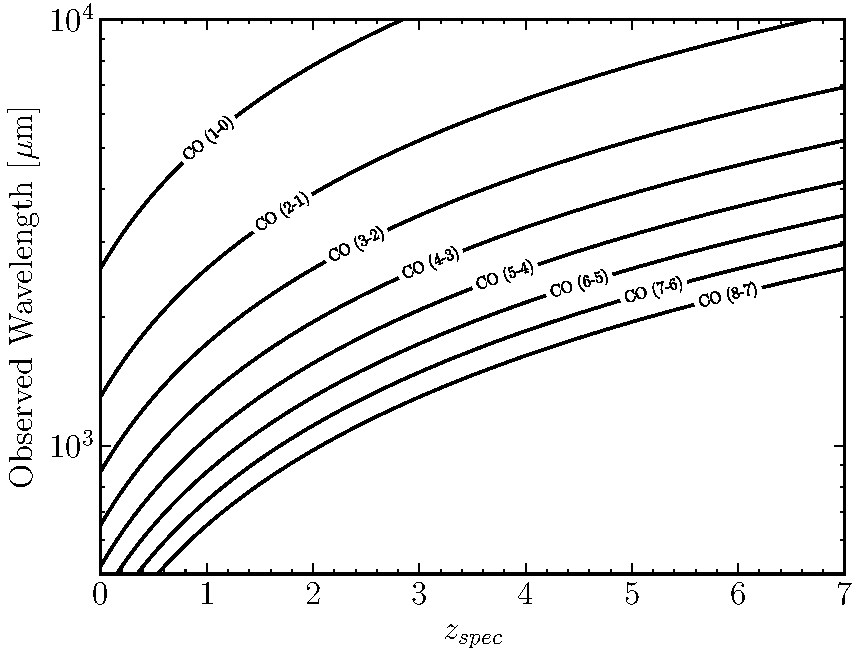
\includegraphics[width=\columnwidth]{Figures/redshift_ladder.pdf}
	\caption{Caption}
	\label{fig:redshift_ladder}
\end{figure}

In this work I study bright infrared sources detected by \textit{Herschel} and the South Pole Telescope (SPT; \citealt{Carlstrom_2011}) that have spectroscopically determined redshifts to test whether their measured dust properties have evolved from the early Universe to the peak epoch of star formation (between 2 $\lesssim z_{\textrm{spec}} \lesssim$ 6). We are also interested in identifying possible diversity in the dust properties of DSFGs and whether differing selection methods influence the type of dust that is observed. I therefore implicity assume in the following work that changes in the properties of the interstellar dust in galaxies can be directly inferred from variations in the spectral index, $\beta$ and the temperature of dust grains.

\section{Sample Creation}
\subsection{South Pole Telescope DSFGs}

A population of IR-bright SMGs selected at 1.4\,mm were obtained from the South Pole Telescope - Sunyarv-Zel'dovich (SPT-SZ) survey (\citealt{Everett_2020}) which covers approximately 2500\,deg$^2$. The depth of this survey reaches $\sim$ 10\,mJy at 1.4\,mm, corresponding to sources detected at greater than 4.5\,$\sigma$ significance. I define our SPT sample as the 81 sources that have had synchrotron dominated systems removed (based on their 1.4\,mm to 2\,mm flux density ratios) and flux-limited to $S_{\textrm{870\,\micron}}$ > 25\,mJy. The high flux density cuts imply that most IR-bright galaxies would be too faint for the SPT sample without having been magnified from gravitational lensing. As shown by \citealt{Weiss_2013}, the average magnification of these sources are $\mu \sim$ 15 (corresponding to intrinsic flux densities of $S_{1.4\,\textrm{mm}}$ = 1 -- 3\,mJy), which is similar to the flux densities of unlensed sources identified from blank field surveys in the sub-mm/mm wavebands (e.g. \citealt{Coppin_2006}; \citealt{Pope_2006}; \citealt{Weiss_2009}) and are thus likely to be representative of this population albeit at higher observed redshifts.

During ALMA Cycle 0 \citealt{Weiss_2013} conducted a blind redshift survey for 26 SPT sources with ALMA's Band 3 receiver (2.6 -- 3.6\,mm). In total 44 line features were identified in the survey as emission lines of $^{12}$CO, $^{13}$CO, CI, H$_2$O and H$_2$O$^+$. The spectra of the 26 sources could be categorized according to the ambiguity of their estimated redshifts: 12 sources had spectra with multiple clear line features, from which a unique redshift solution can be found from the ALMA scans alone; 11 had a single line feature for which other spectroscopic or photometric measurements would be requied to constrain the redshift; and three sources for which no line features were observed. The same observing strategy was used during ALMA Cycle 1 by \citealt{Strandet_2016} to extend the redshift survey of \citealt{Weiss_2013} with an additional 15 sources observed in ALMA Band 3. For sources with a single CO line detection during Cycle 0, \citealt{Strandet_2016} present ALMA 1\,mm (Band 6) follow-up observations and, when still not satisfactory, follow-up observations were made with the First Light APEX Submillimetre Heterodyne receiver (FLASH; \citealt{Heyminck_2006}), the Swedish-ESO PI receiver (SEPIA; \citealt{Billade_2012}) and the Z-spec camera (\citealt{Naylor_2003}) onboard the Atacama Pathfinder Experiment (APEX) targeting CO and [CII] lines for those that remained unambiguous during Cycles 0 and 1. Lastly, \citealt{Reuter_2020} concluded the SPT redshift survey during ALMA Cycles 3, 4 and 7 by presenting spectra for the remaining 40 of the total 81 sources that had yet to be scanned. This resulted in 41 new spectroscopic redshifts. The culmination of these studies is a sample of 81 SPT-selected DSFGs  each with a spectroscopic redshift in the range 1.9 < $z_{\textrm{spec}}$ < 6.9; the median redshift of the sample being $z_{\textrm{median}}$ = 3.9$\pm$0.2 (\citealt{Reuter_2020}).

The SPT-DSFGs have photometric coverage that fully traces the SED peak and Rayleigh-Jeans (R-J) tail of the dust emission for all sources. Most of the SPT sample have coverage that spans at least observed wavelengths between 250\,\micron and 3\,mm. This photometry includes flux densities measured at 250-, 350- and 500\,\micron (\textit{Herschel}-SPIRE), 870\,\micron (APEX-LABOCA), 1.4- and 2\,mm (SPT) and 3\,mm (ALMA). For a subset of 65 sources, 100- and 160\,\micron flux densities were measured with \textit{Herschel}-PACS. The flux densities from \textit{Herschel} were estimated by fitting a Gaussian to the SPIRE counterparts and taking the peak as the flux density at 250-, 350- and 500\,\micron, or by using apertures of 7' and 10' to extract the flux density at 100- and 160\,\micron. The LABOCA, SPT and ALMA flux densities were taken to be the peak flux density of the point sources observed on the respective continuum maps. For the 3\,mm observations with ALMA, this was estimated from the continuum maps obtained during the blind redshift search. Given the range of redshifts, the SPT sources have a minimum photometric coverage between rest frame wavelengths 83\,\micron $\lesssim \lambda_{\textrm{rest}} \lesssim$ 380\,\micron meaning that the peak of the dust emission at $\sim$ 100\,\micron is always constrained and the Rayleigh-Jeans tail is well sampled (note that in Section [...]\todo[color=green]{Add section reference when written} I place further constraints on which sources are included in this study based on the number of photometric constraints available on the R-J tail). The complete set of photometric observations for the SPT DSFGs can be found in Appendix D of \citealt{Reuter_2020} and in Appendix \ref{app:SPT_DSFG_photometry} including the estimated magnifications of each source due to gravitational lensing as measured by \citealt{Spilker_2016}. In the cases where a magnification could not be measured, the average value of $\mu$ = 5.5 is used.

\subsection{The HerBS Sample}

A second sample used in this study comes from the \textit{Herschel} Bright Sources (HerBS; \citealt{Bakx_2018}) catalogue, a sample selected from the brightest high-redshift sources detected from the H-ATLAS project. Using the SED template derived by \citealt{Pearson_2013} to represent typical H-ATLAS sources (see Section \ref{sec:phot_z_Herschel}), \citealt{Bakx_2018} estimated the redshift of each source and selected those that have a measured photometric redshift > 2 and are observed at a 500\,\micron flux density > 80\,mJy. Initially the sample consisted of 223 sources, but having removed nearby galaxies and known blazars (\citealt{Negrello_2010}; \citealt{Lopez-Caniego_2013}), the HerBS sample is reduced to 209 SMGs. Presented with the catalogue are observations at 850\,\micron with the SCUBA-2 instrument (\citealt{Holland_2013}) on the James Clerk Maxwell Telescope (JCMT) for 203 sources. A detected source with SNR$_{850\,\micron}$ > 3 and offset from the \textit{Herschel} source < 10" is observed for 159 galaxies. Given that the sensitivity of \textit{Herschel}-SPIRE observations are poor beyond redshifts z $\sim$ 2 [...]\todo[color=orange]{Give some justification here}, the selection of galaxies in the HerBS sample is limited to very bright, rare sources. A large percentage of the sample are thus lensed ultraluminous IR galaxies (ULIRGS) with far-IR luminosities in the range $10^{12} L_\odot < L_{FIR} < 10^{13} L_\odot$ and hyperluminous IR galaxies (HyLIRGS) with $L_{FIR} > 10^{13} L_\odot$.

Spectroscopic redshifts are obtained for a subset of sources in the HerBS catalogue (selected from the H-ATLAS South Galactic Pole field) as part of the Bright Extragalactic ALMA Redshift Survey (BEARS: \citealt{Urquhart_2022}; \citealt{Bendo_2023}; \citealt{Hagimoto_2023}). \citealt{Urquhart_2022} targeted 85 sources for CO line emission with ALMA and presented spectroscopic measurements for 71 sources associated with 62 HerBS fields (the ALMA Band 4 images with angular resolution of $\sim$ 2" revealed that only half of the fields contained just a single source, while several contained two or more objects with similar spectroscopic redshifts - suggesting possible locations of physially associated galaxies or single sources being lensed by a foreground deflector). The BEARS spectral line survey started in ALMA Cycles 4 and 6 using the Band 3 receiver of the Atacama Compact Array (ACA) and continued during Cycle 7 in Bands 3 and 4 with the ALMA 12\,m Array. All sources with a spectroscopic redshift have Band 3 observations with the 12\,m Array, 74 of which also have Band 3 observations. The 11 remaining sources without Band 3 observations from the 12\,m Array depend on the ACA. As shown in Figure \ref{fig:redshift_ladder} \todo[color=orange]{Check that this is illustrated} the coverage of Bands 3 and 4 allows for the detection of CO lines between (2 -- 1) and (6 -- 5) depending on the redshift of the source; \citealt{Urquhart_2022} find that line detections are primarily found from the CO(3 -- 2), (4 -- 3) and (5 -- 4) transitions (38, 36 and 28 sources respectively). The frequencies of the spectral lines are transformed to redshift solutions using the graphical method described in \citealt{Bakx_2022} and, in doing so, find redshifts for 59 sources based on multiple spectral lines suggesting an unambiguous redshift. An additional 13 sources with emission from a single line have redshift solutions that can be relied upon since the CO emission is notably bright. Since adjacent CO lines typically have similar integrated line fluxes, alternative redshift solutions can be excluded when a single strong emission line is present. HerBS sources are retained in this study if they have spectroscopic redshifts determined from a single CO line.

In the cases where the HerBS source is deblended in the ALMA images I assume that the redshift of the group is the average spectroscopic redshift of all components, providing they are within 0.1 of each other. If there is only a single redshift corresponding to one of the components (and the redshift corresponding to the integrated emission of all sources is not provided), I assume that the redshift is applicable for the whole field. While \citealt{Bendo_2023} show that the brightest component (alphanumerically labelled A for each source) produces < 80\% of the total emission at 2\,mm, it is only in 4 fields (HerBS-56, -131, -138 and -146) that the spectroscopic redshift is assumed from components that does not include the brightest.

The photometry available for HerBS sources covers a similar range to the SPT sample: \textit{Herschel}-PACS (100-, 160\,\micron), \todo[color=orange]{Include these values} \textit{Herschel}-SPIRE (250-, 350-, 500\,\micron), SCUBA-2 (850\,\micron), ALMA (2-, 3\,mm). The ALMA flux densities were serendipitously estimated from the continuum of the spectrosopic survey. I also include snapshot continuum observations in ALMA Band 6 (1.1 -- 1.4\,mm) for a selection of ultra-red objects from the H-ATLAS that were taken as part of project 2018.1.00526.S (\textit{3000 dusty starbursts at z > 4}). For sources where the reduced angular resolution of the ALMA beam resolves the HerBS source into multiple components, \citealt{Bendo_2023} report the integrated flux densities of all objects if they lie within twice the FWHM of the ALMA beam, or if they are connected by structures that are themselves detected at greater than 3$\sigma$ significance. I preferentially chose to use the integrated fluxes for each HerBS source if available, or failing this, combine fluxes of individual components providing they are all detected. For example, the HerBS-63 field showed two detected ALMA sources in the Band 4 images, while a third source appeared in the Band 3 image misaligned with the other two. The third component (HerBS-63C) may not have been detected at 2\,mm because of poor sensitivity at the edge of the 3\,mm image or because it contains some contribution from AGN emission making it much brighter at longer wavelengths. In either case this inhibits us from knowing the integrated flux in both bands for all components, assuming that they may all be physically related, and so has been left out of the sample used here. In this sense I have taken a cautious approach to combining photometry. The shorter selection wavelength compared to the SPT sample leads to a narrower and lower redshift distribution; the minimum and maximum redshifts obtained by \citealt{Urquhart_2022} were $z_{\textrm{min}} = 1.407$ and $z_{\textrm{max}} = 4.509$. Considering the spectroscopic redshifts of the HerBS sources used in this study, the minimum photometric coverage is between rest frame wavelengths of $\sim$ 97\,\micron and $\sim$ 392\,\micron. The photometric coverage of HerBS galaxies has been tabulated in Appendix \ref{app:HerBS_photometry}.

\todo[color=red]{Put all numbers in math mode.}

\subsection{The Combined SPT and HerBS Samples}

In total there are 143 sources with a spectroscopic redshift across the two samples (81 SPT, 62 HerBS-BEARS). However, as we are interested in measuring the galaxy-integrated dust emissivity spectral index of each source, which is characterized by the slope of the emission on the R-J side of the Planck function, I make it a requirement of the final samples that there are at least two observations at observed wavelengths greater than 1\,mm for each galaxy. This has the effect of reducing the final group of galaxies studied here to 109 (79 SPT and 30 HerBS-BEARS). In the following I treat the two populations separately to highlight any potential differences that may result from the different selection wavelengths and flux limits. The redshift distribution is illustrated in Figure \ref{fig:spt_herbs_redshift}.

\begin{figure}
	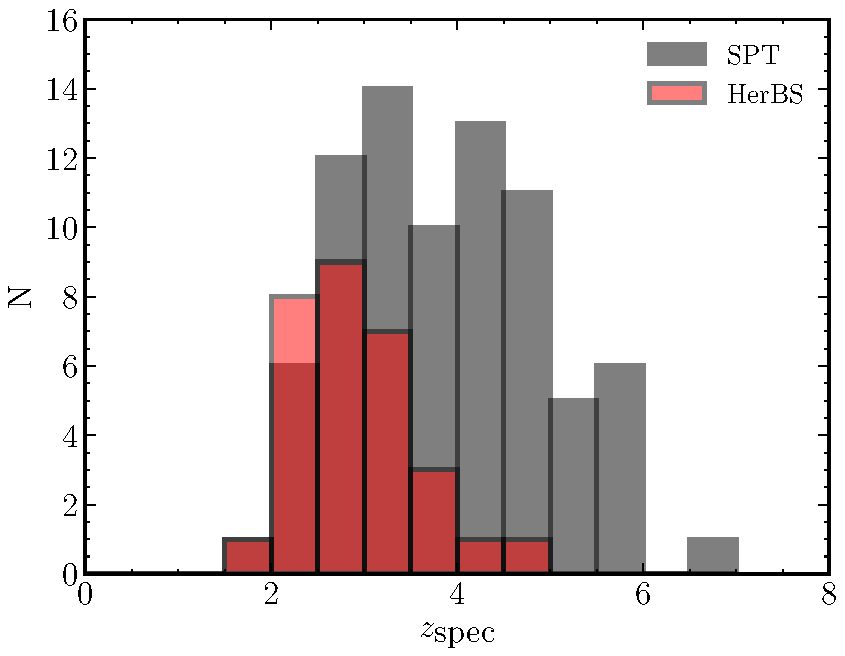
\includegraphics[width=\columnwidth]{Figures/spt_herbs_redshift_distribution.pdf}
	\caption{The spectroscopic redshift distributions for the SPT-DSFG (grey) and HerBS (red) samples.}
	\label{fig:spt_herbs_redshift}
\end{figure}

\section{Far-Infrared and Sub-mm Colours}

A first estimate on the average dust properties of the two samples can be made by comparing their far-IR colours (which I define as the ratio between two flux densities in the FIR regime) with the predictions made using isothermal blackbody models. Previous studies have shown that FIR colours can be used as a proxy for dust properties (e.g. \citealt{Boselli_2010}; \citealt{Boselli_2012}; \citealt{Remy-Ruyer_2013}; \citealt{Smith_2019}) depending on the part of the FIR spectrum that the colour samples. For example, smaller wavelengths involving the \textit{Herschel}-PACS and \textit{Herschel}-SPIRE flux densities are more sensitive to changes in the dust temperature, while longer wavelengths are more sensitive to variations in the dust emissivity spectral index. In Figure \ref{fig:spt_herbs_colour_redshift} I show a selection of colours using flux densities between \textit{Herschel}-SPIRE 250\,\micron and ALMA 3\,mm that progressively travel across the spectrum from sampling the peak of thermal dust emission to the R-J tail. Using an isothermal modified blackbody model of the form $S_\nu \propto \frac{\nu^{\beta+3}}{e^{h \nu/kT} - 1}$, I predict the dependence of FIR colour on redshift for three combinations of dust temperature, $T_{\textrm{dust}}$, and $\beta$ ([T=30\,K, $\beta$=2], [T=30\,K, $\beta$=1.8] and [T=40\,K, $\beta$=2]). It can be seen that the assumed dust temperature has a significant effect on the location of the SED track for all FIR colours, while it is noticable that a change in $\beta$ has a larger effect on the observed colours at the longest wavelengths. 

Assuming for now that the dust emissivity index is well represented by $\beta \sim 2$ for all galaxies, then the FIR colours of most sources can be explained by a range of dust temperatures between T = 30 -- 40\,K assuming optically thin dust emission. There are notable exceptions, including a selection of SPT sources with high $S_{250\,\textrm{\micron}}/S_{500\,\textrm{\micron}}$ \todo[color=red]{Likely the 500um data, what does this imply?} and sources from both samples with high $S_{500\,\textrm{\micron}}/S_{3\,mm}$. At first this might suggest sources with large dust temperatures and/or high values of $\beta$, but other common culprits could be leading to these deviations from the bulk population. The most likely are the uncertainties on the flux density measurements or biases due to the choice of photometry. We note that our galaxies contain a combination of photometry obtained from single-dish observations (e.g. \textit{Herschel}, JCMT and SPT) and interferometers (ALMA). With their varying angular resolutions, emission observed with one instrument may be missed by another. In particular, we might expect that when ALMA resolves the single sources observed in the \textit{Herschel} wavebands into multiple components, some emission is lost giving the impression of higher FIR colours and thus higher dust temperatures and/or higher $\beta$.

In general, the SPT and HerBS galaxies occupy similar regions of the colour-redshift space, suggesting that the intrinsic dust properties of the two samples are likely to be similar. Given the scatter observed around the MBB models, it is appears unlikely that a single value of dust temperature and $\beta$ represents the observed SED of each galaxy equally well. \todo[color=red]{Description on how well the models represent the data - normalized distances should resemble a standardized normal distribution and colour-colour plots should be strongly correlated if the SEDs are well approximated by a single MBB with fixed beta.} 

The above results suggest that a single dust model assuming a constant $\beta$ value cannot explain the distribution of SEDs observed among the two populations. We are interested in ascertaining a single galaxy-integrated $\beta$, thus we must turn to fitting the observed SEDs individually to measure their dust properties. In the following I address two important questions about the properties of dust in high-redshift galaxies: i) is there diversity in the dust properties of high-redshift DSFGs? and ii) did these properties evolve over time? 


\begin{figure}
    \centering
    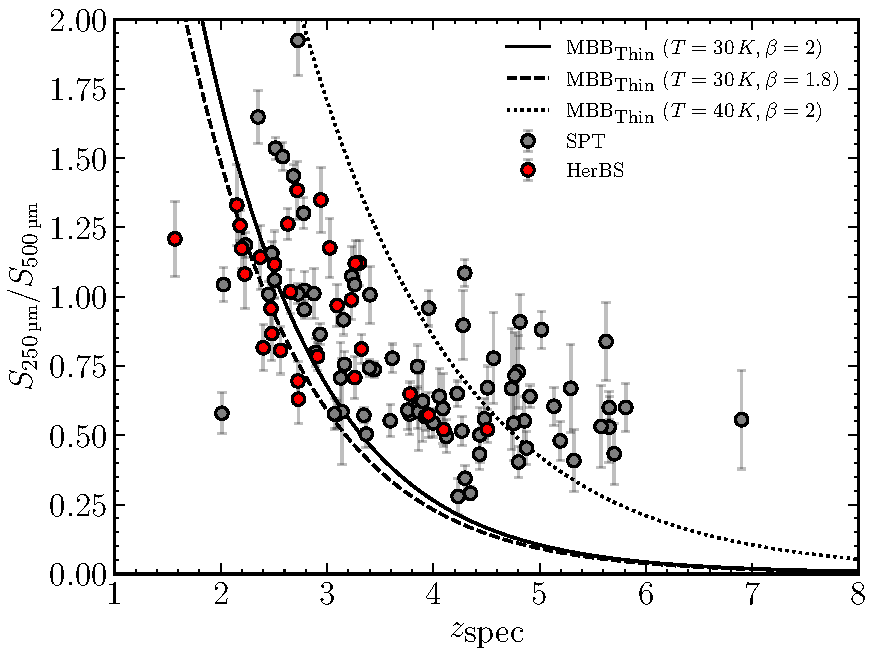
\includegraphics[width=0.5\columnwidth,height=0.26\textheight]{Figures/spt_herbs_colour_250_500.pdf}
    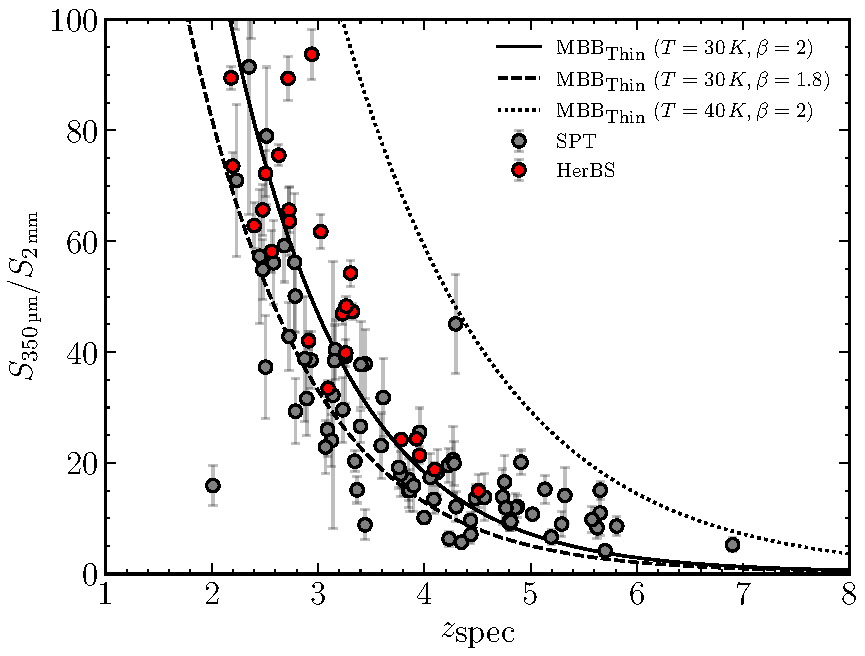
\includegraphics[width=0.5\columnwidth,height=0.26\textheight]{Figures/spt_herbs_colour_350_2000.pdf}
    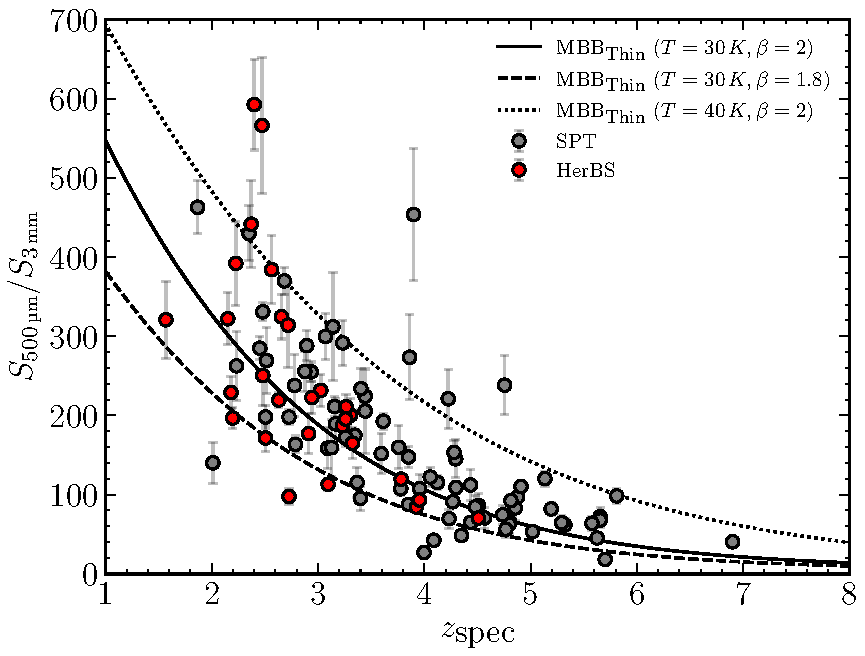
\includegraphics[width=0.5\columnwidth,height=0.26\textheight]{Figures/spt_herbs_colour_500_3000.pdf}
    \caption{Colour-redshift plots of X/X, X/X and X/X against spectrosopic redshift. The SPT sources are illustrated with grey circles and the HerBS sample as red circles. The predictions from three modified blackbody models assuming optical thin dust ([T = 30\,K, $\beta$=2], [T = 30\,K, $\beta$=1.8] and [T = 40\,K, $\beta$=2]) are plotted as solid, dashed and dotted black lines respectively.}
    \label{fig:spt_herbs_colour_redshift}
\end{figure}
\todo[color=orange]{Confirm which colours I am plotting here. They need only be progressively sampling longer wavelengths.}


\section{The Modified Blackbody Model}

I modelled the FIR to millimeter spectra by fitting a single MBB model combined with a mid-IR power law to all sources. In the FIR to mm regime the SED is dominated by a modified Planck function that represents the cold dust reservoir from which most of the mass of dust in the ISM is contained. This "cold" dust resides in the diffuse ISM and is heated by the ambient interstellar radiation field. However, a lower fraction of dust by mass radiates at hotter temperatures, heated by nearby star-forming regions, young OB stars or AGNs which contributes substantially to a galaxy's IR luminosity and dominates the emission at rest frame wavelengths $\lesssim$ 70\,\micron. This mid-IR component can be approximated using a power law of dust temperatures of the form $S_\nu \propto \nu^{-\alpha}$, where a lower value of $\alpha$ represents a higher fraction of emission emananting from sources other than the cold reservoir of dust, and higher values asymptotically tending towards a modified blackbody, representing a single temperature of dust.

The modified blackbody form is a direct result of the radiative transfer equation, $\frac{dI_\nu}{ds} = -\kappa_\nu \rho I_\nu + j_\nu \rho$, where $\kappa_\nu$ represents the opacity of the dust, $\rho$ is the density, $j_\nu$ represents the emissivity of the dust and $I_\nu$ is the spectral radiance (per unit area). If we define the source function, $S_\nu$ as $j_\nu/\kappa_\nu$ and the frequency dependent optical depth as $d\tau_\nu = -\kappa_\nu \rho ds$, then the radiative transfer equation becomes $\frac{dI_\nu}{ds} = I_\nu - S_\nu = I_\nu - B_\nu$, where we have used the fact that at local thermal equilibrium (LTE) the source function is equal to the Planck function, $B_\nu(T)$. The solution to the radiative transfer equation takes the form $I_\nu = (1 - e^{-\tau_\nu}) B_\nu(T)$. Given that the spectral radiance is proportional to the flux density at a given frequency, we can rewrite this as the modified blackbody model:

\begin{equation}
	S_\nu = \Omega(1 - e^{-\tau_\nu}) B_\nu(T),
\label{eq:modified_blackbody_omega}
\end{equation}

where $\Omega$ represents the solid angle subtended by the galaxy. Assuming the distance between the source and observer is $D$, then in the limit where $D$ is very large, the solid angle tends to the ratio between the projected area of the source on the sky and the square of the distance. Therefore,

\begin{equation}
	S_\nu = \frac{\mu A}{D^2}(1 - e^{-\tau_\nu}) B_\nu(T),
\label{eq:modified_blackbody_area}
\end{equation}

where $A$ is the area of the source and I have included a multiplicative factor $\mu$ to account for the possibility of magnification due to gravitational lensing. For any galaxy where there is no evidence to suggest that gravitational lensing is magnifying the source, we may set $\mu = 1$.

The optical depth, $\tau_\nu$

\section{SED Fitting of DSFGs}
\subsection{Residuals and Potential Biases in Photometry}
\subsection{Posterior Distributions}
\subsection{The Dust Emissivity Spectral Index - Dust Temperature Degeneracy}
\section{Accuracy of Dust Parameters}
\subsection{Simulations of SPT and HerBS Sources}
\subsection{Results of Simulations}
\section{The Properties of Dust in DSFGs}
\subsection{The Diversity of Dust Emissivity Spectral Indices and their Evolution with Redshift}
\subsection{The Diversity of Dust Temperatures and their Evolution with Redshift}
\subsection{Implications of Evolving Dust Properties between 2 < z < 6}
\section{Conclusions}

\listoftodos

\chapter{Properties of SMGs from Radio Observations}
\label{chapter:Radio_Identifications}
\chapquote{"Video killed the radio star."}{The Buggles}{1979}

\section{Introduction}

\section{The Far-Infrared/Radio Correlation}

For samples of star forming galaxies in the local and high redshift universe there is a well observed correlation between the far-infrared and radio emission (e.g. \citealt{Dickey_1984}; \citealt{deJong_1985}; \citealt{Helou_1985}; \citealt{Condon_1992}; \citealt{Barger_2000}; \citealt{Yun_2001}; \citealt{Garrett_2002}; \citealt{Appleton_2004}; \citealt{Ibar_2008}; \citealt{Seymour_2009}; \citealt{Sargent_2010}), that remains nearly linear over multiple orders of magnitude in far-infrared luminosity ($10^{9} \lesssim L_{\textrm{FIR}} [L_{\odot}] \lesssim 10^{12.5}$). The small scatter in this relation is often attributed to the "calorimeter model" (\citealt{Voelk_1989}; \citealt{Lisenfeld_1996}; \citealt{Lacki_2010}), which ascribes the far-infrared and radio emission to common stellar sources. In this model, galaxies are assumed to be opaque to UV light from massive OB stars which gets absorbed by the dust in the ISM and reradiated in the far-infrared. Observations in the far-infrared and sub-mm are thus sensitive to the cold dust that reradiates the energy from young stars. These stars quickly come to the end of their lives, exploding as Type II supernovae producing cosmic ray electrons and positrons. Most of their energy gets radiated in the radio as synchrotron radiation when interacting with the magnetic fields of the supernova remnant. The radio continuum is therefore a tracer of recent, obscured star formation.

Despite a higher scatter for high redshift SMGs than with local samples, the far-infrared/radio correlation (FIRC) still holds at increasing redshift (\citealt{Ivison_2010a}; \citealt{Ivison_2010b}). {\color{red}Small description on evolution of FIRC with redshift.}

The appearance of a correlation at all redshifts and luminosities has facilitated studies that use the radio emission as an unbiased tracer of obscured star formation in dusty galaxies (\citealt{Kennicutt_2012}). By making use of the tight correlation (as well as the benefits we outline in the following section), we can identify counterparts to single dish sub-mm observations with large beams with greater confidence than we would expect from the optical or near-infrared. This allows for better characterization of the properties of SMGs and allows us to study the cosmic star formation history to higher redshifts (\citealt{Madau_2014}; \citealt{Delhaize_2017}; \citealt{Novak_2017}).

\section{Identifying Multiwavelength Counterparts to SMGs via Radio IDs}

As illustrated in Chapter \ref{chapter:Data_Release_3}, SMGs that are detected with single dish sub-mm telescopes with low angular resolution will likely include multiple galaxies in the optical or near-infrared within the beam width. This is a particular problem for \textit{Herschel} where even the smallest beam size at 250\,\micron\ has a FWHM of $\sim$ 18\,arcsec. The possibility of tightly clustered SMGs (\citealt{Blain_2004}) and with a higher surface density of optical counterparts, deciding unambiguously on the source of the sub-mm emission is difficult. This is further compounded by their intrinsic faintness due to the dust obscuration. The optimal way to overcome the problem of poor resolution is to follow up with millimetric or longer wavelength interferometric observations. In the following sections we detail a method for identifying radio counterparts to \textit{Herschel} sources in order to secure unambiguous multiwavelength counterparts to our sub-mm galaxies. The following is a list of benefits of using the radio emission to select counterparts throughout the electromagnetic spectrum.

\begin{enumerate}
    \item Star forming galaxies produce a lot of synchrotron emission. This allows us to take advantage of the FIRC to locate the galaxy emitting radiation in the far-IR. Compared to searches in other wavelengths, such as using the Likelihood Ratio to identify optical counterparts, the search for identifications is not solely motivated by their position and brightness, but also by the physical link between the two objects due to their common source.
    \item Even when considering the deepest radio maps, the low surface density of radio sources means that the probability of chance positoinal coincidences with a sub-mm source is relatively unlikely. As a result, we can have a reasonable confidence in some association between objects when we do observe radio sources in close proximity to the sub-mm position (\citealt{Ivison_2002}; \citealt{Borys_2004}). In most cases (as we shall validate in this study), radio sources are sufficiently rare that finding an object within the positional uncertainty of the sub-mm beam almost always results in a robust identification.
    \item When a secure radio counterpart is identified, the positional accuracy ($\sim$ 1\,arcsec for the Karl G. Jansky Very Large Array (VLA) at 1.4\,GHz and $\sim$ 0.75\,arcsec at 3\,GHz) allows for a unambiguous identification with an optical or infrared galaxy counterpart. By locating these galaxies via the radio identification, we predict a low false identification rate of the SMG with the optical counterpart, allowing us to determine their morphologies, colours, magnitudes, stellar masses and more with greater confidence.
\end{enumerate}

While the radio emission from star-forming galaxies allows for secure identification of counterparts across the spectrum, it also has several drawbacks. The following is a list of disadvantages to using radio emission.

\begin{enumerate}
    \item Our understanding of the radio-selected SMG population is likely to be skewed by selection effects. The negative k-correction in the far-infrared arises due to the steep Rayleigh-Jeans part of the SED and allows for nearly equal detection of dusty galaxies at $z \sim 0.5$ as $z \sim 8$ for longer wavelengths where this effect is most pronounced (\citealt{Blain_2002}). The radio, however, suffers from a strong positive k-correction which causes a bias against high redshift galaxies ($z > 3$). This means that a substantial fraction of SMGs remain undetected in the radio due to the lack of sufficiently deep radio data. Despite this, we note that such deep radio data would produce a redshift distribution of SMGs much wider than we could obtain with the coverage of the SGP in the near-infrared (Chapter \ref{chapter:Data_Release_3}).
    \item Despite the benefit of the FIRC in locating radio galaxies in close proximity to SMGs, the correlation also causes a preference for the brightest SMGs, which may not be a representative sample of the full SMG population.
    \item Interferometry has been used to show that for sub-mm sources in which we observe multiple radio galaxies in close proximity, in $\sim$ 80\% of cases the sub-mm emission is associated from only one of the radio sources. This leads to an ambiguity as to the nature of some apparent multiple systems when interferometry is not available.
    \item Potentially the most pivotal drawback for the identification of sub-mm emitting galaxies, is the sky coverage from radio surveys. While we have large sky surveys in the sub-mm such as \textit{Herschel}-ATLAS, using radio data for large area sub-mm surveys is not yet practical. Future radio surveys such as the Square Kilometre Array (SKA) and recent wide-area surveys with the Low-Frequency Array (LOFAR) allow us to produce larger samples of SMGs to understand their stellar properties.
\end{enumerate}

Many studies (e.g. \citealt{Eales_2009}; \citealt{Dye_2009}) adopt a frequentist approach to searching for possible radio counterparts close to the sub-mm position. This often involves using Monte Carlo simulations to estimate the probability that a given counterpart is located near the source by chance. The advantage of using a frequentist approach over a Bayesian method (Chapter \ref{chapter:Data_Release_3}) is that it does not require assumptions to be made on the form of the sub-mm positional errors, given that they are poorly known due to source confusion. As will be shown later, we can use the results of a frequentist approach to infer the distribution of positional errors. Despite this benefit, a frequentist approach would not have been appropriate for the VIKING counterparts we identified in the SGP because of their higher surface density {\color{red}[... Check my reasoning here ...]} 

\section{Identifying Radio IDs to \textit{Herschel} Sources in COSMOS}

In the following sections we identify radio counterparts to \textit{Herschel} detected sources in the Cosmic Evolution Survey (COSMOS). We applied the frequentist method of \citealt{Lilly_1999}, which differs from the Bayesian Likelihood Ratio method in that it searches for objects close to the sub-mm source and estimates the probability that each object is a chance alignment, rather than estimating the probability the two are physically associated. COSMOS is a deep, wide area survey of an equatorial two square degree field centered at R.A $+150.12^{\circ}$ and declination $+2.21^{\circ}$ (\citealt{Scoville_2007}). The field has been observed with many space-based (e.g. \textit{Hubble Space Telescope}, \textit{Spitzer}, \textit{Chandra} and \textit{Herschel}) and ground-based telescopes (e.g. Keck, VLA and UKIRT), resulting in multiwavelength data that spans from the X-ray to radio wavelengths. The high sensitivity and resolution of these data sets over a sufficiently large area, allows for comprehensive studies on the co-evolution of galaxies (\citealt{Schreiber_2018}; \citealt{Stockmann_2020}; \citealt{Valentino_2020}), star formation (\citealt{Gruppioni_2013}; \citealt{Novak_2017}), large scale structure (\citealt{Scoville_2013}; \citealt{Laigle_2018}) and AGN (\citealt{Prescott_2006}; \citealt{Heintz_2016}). 

\subsection{\textit{Herschel} Observations in COMSOS}

The \textit{Herschel} detected sources that we study in this work were taken as part of the \textit{Herschel} Multi-tiered Extragalactic Survey (HerMES; \citealt{Oliver_2012}). HerMES is a deep far-infrared imaging survey of some of the most well-studied blank extragalactic fields. As part of the survey, the COSMOS field was observed with SPIRE over the full two square degrees.

The survey design of HerMES allowed for the detection of a wide range in far-IR luminosities by targeting high luminosity objects which are bright but rare in wide, shallow surveys and the lower luminosity objects, which are faint but common, in deep, narrow surveys.

{\color{red}[More description on the COSMOS field and the number of Herschel sources.]}

\subsection{VLA Observations in COSMOS}

The VLA-COSMOS 3\,GHz Large Project (\citealt{Smolcic_2017a}; \citealt{Smolcic_2017b}; \citealt{Smolcic_2017c}) was a radio continuum survey covering 2.6 square degrees, enclosing the two square degrees of the COSMOS field, with a mean rms sensitivity of $\sim$ 2.4\,$\mu$Jy beam$^{-1}$ and an exceptional angular resolution of 0.75\,arcsec at 3\,GHz. Observations of the COSMOS field were taken in the S-band (2 -- 4\,GHz) for a total of 384 hours. The benefit of the S-band observations are the large effective bandwidth ($\sim$ 2\,GHz) and large field of view, allowing for fast coverage of a field such as COSMOS. The survey recovered 10,899 radio source components with SNR greater than five, 67 of which had been merged into multicomponent sources, resulting in a total of 10,830 radio sources. The VLA-COSMOS 3\,GHz catalgue builds on the existing 1.4\,GHz VLA catalogue (VLA-COSMOS Large and VLA-COSMOS Deep projects: \citealt{Schinnerer_2004}; \citealt{Schinnerer_2007}; \citealt{Schinnerer_2010}) of 2,865 1.4\,GHz-detected (L-band) radio sources. The increased sensitivity of the S-band compared to the L-band allows for an increase in the number of detected sources a factor approximately four times greater over a similar sky area, though we note that the sources detected in the VLA-COSMOS 3\,GHz catalogue are typically fainter.

The VLA-COSMOS 3\,GHz Large Project is the deepest radio continuum survey for a field as large as that of COSMOS, which combined with the extensive multiwavlength described above, makes it a unique survey for studying the composition of the radio-detected galaxy population. As we shall explore later, the \textit{Herschel}-detected sources that are coincident with radio sources in COSMOS make for an unparalleled set of far-IR selected galaxies with known stellar properties. With such confidence in the stellar properties of dusty star forming galaxies, this data set provides an opportunity to precisely determine the galactic environments conducive to such high star formation rates and allow us to make predictions about the radio populations from future surveys that will be able to cover the larger areas of sky already mapped in the far-IR and sub-mm. The robust radio IDs to \textit{Herschel} sources will help facilitate the identification of similar dusty galaxies in large surveys from the likes of the SKA (\citealt{Dewdney_2009}) and the Next Generation Very Large Array (ngVLA), as well as their precursors such as the Australian Square Kilometre Array Pathfinder (ASKAP: \citealt{Johnston_2007}), the \textit{enhanced} Multi Element Remotely Linked Interferometer Network (\textit{e}-MERLIN), LOFAR and MeerKAT (\citealt{Jonas_2009}).

The sample studied here are the \textit{Herschel}-detected and VLA-detected sources that lie within an overlapping region as shown in Figure \ref{fig:sky_map}. We define a square region from R.A $+149.29^{\circ}$ to $+150.95^{\circ}$ and declination $+1.45^{\circ}$ to $+3.04^{\circ}$. This 2.64 square degree region contains 7,230 (64.6\%) \textit{Herschel} and 10,826 ($\sim$ 100\%) radio sources.

\begin{figure}
	\centering
	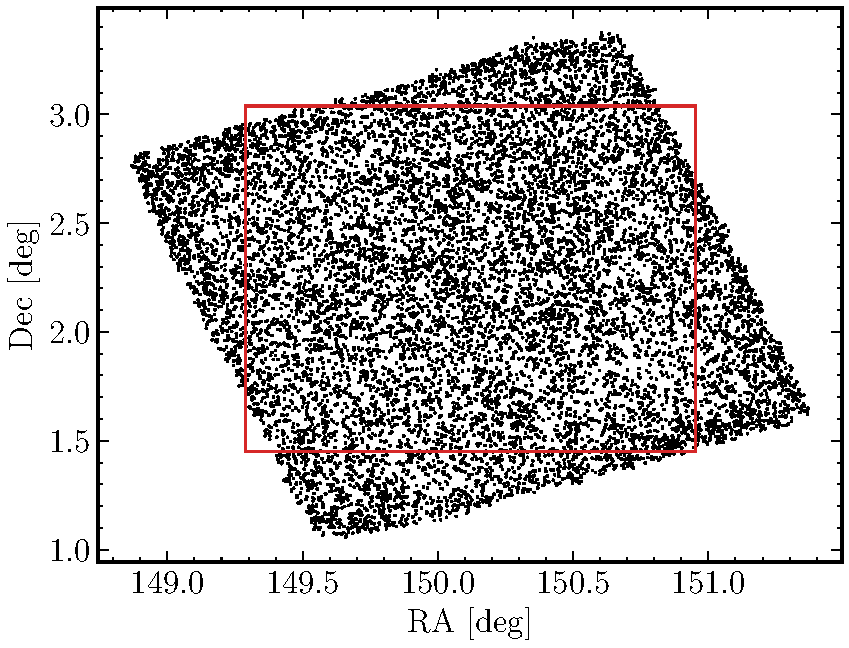
\includegraphics[width=0.75\columnwidth]{Figures/sky_map.pdf}
	\caption{{\color{red} Caption.}}
	\label{fig:sky_map}
\end{figure}

\subsection{The COSMOS2020 Catalogue}

{\color{red}Description of the COSMOS2020 catalogue.}

\subsection{Calculating the Significance of Associations}

To predict the probability that a sub-mm-radio pair is a significant association we could use the corrected Poisson probability defined by \citealt{Downes_1986}. This measures the Poisson probability that a radio source of a given flux density could lie at the observed distance from the source by chance. In this original paper the Poisson probability is defined as $P = 1-e^{-\mu}$ where $\mu = \pi r^2n$. Here $r$ is the radial offset between the source and radio counterpart and $n$ is the surface density of objects brighter than the radio counterpart. While a low value of $P$ does not confirm that the radio source is the correct ID for the sub-mm source, it suggests that the two are likely associated. A low value of $P$ can be interpreted in a number of ways. First, the radio source could be the true counterpart of the sub-mm source. Second, the counterpart could be one of a group of galaxies that collectively contribute to the flux density observed in the sub-mm. This is a very plausible case for the sources in our sample given the large beam sizes for \textit{Herschel}-SPIRE. Third, the low value of $P$ could be the result of an indirect association with the source, for example, due to clustering with the true ID or from the effects of gravitational lensing (although in the case of gravitational lensing this seems unlikely for our sample, as this would suggest that the lenses are as dust obscured as the background sources).

We used the method of \citealt{Lilly_1999} which applies the principles of the Poisson probability from \citealt{Downes_1986} in a Monte Carlo approach. The method, which is given in detail in \citealt{Dye_2009}, is as follows. First, we generate a set of $N$ random positions in the area common to both the sub-mm and radio surveys. Next, we identify all radio sources within some maximum radius, $r_{\textrm{max}}$, from each random position. For each radio source we measure the quantity $S = r^2n$, where $r$ and $n$ take the same definitions as earlier. The minimum value of $S$ for each source (corresponding to the most significant association in the case where multiple radio sources are observed) is retained. This defines our distribution, $D(S)$, which represents the distribution of $S$ values for random chance alignments. This distribution allows us to determine the probability of an observed radio source with $S = S_i$ and within $r_{\textrm{max}}$ of a sub-mm source being a random interloper. This is computed as:

\begin{equation}
    P(< S_i) = \frac{1}{N}\int_0^{S_i}D(S) dS.
    \label{eq:probability_frequentist}
\end{equation}

As is often assumed, we consider a radio source to be a secure identification if it has $P < 0.05$, suggesting that there is less than a 5\% probability that such a radio source would be observed by chance (e.g. \citealt{Ivison_2002}; \citealt{Ivison_2005}; \citealt{Pope_2006}). Depending on the surface density of radio galaxies, the maximum value of $P$ will often be less than one as some fraction of the randomly chosen positions will not contain any radio sources within $r_{\textrm{max}}$. 

The value of $r_{\textrm{max}}$ is an important choice. While a smaller search radius reduces the number of potential IDs and increases the likelihood of missing a true counterpart, a larger radius causes a greater probability of observing a background object and thus matching the source with an unrelated radio galaxy. A further problem is that too large a search radius causes overlapping fields which could lead to radio sources being connected to more than one sub-mm position. Previous studies (e.g. \citealt{Dye_2009}) have defined the maximum radius using a probabilistic balance between these two competing effects, finding the radius where the expected number of false counterparts in the final sample equals the expected number of true counterparts that are excluded. In this study we are attempting to define a clean sample of radio matched \textit{Herschel} sources, such that our multiwavelength counterparts from the COSMOS field represent a near complete and thorough description of the optical to radio properties of \textit{Herschel} detected sources. As we shall show later, this sample could provide a useful starting point for identifying dusty galaxies in future large area surveys (e.g. \textit{Euclid}) given that our sample will define some subpopulation of the COSMOS survey. For this reason, we are less interested in retaining the appropriate size of the sample, but rather in minimizing the number of falsely identified counterparts that would obfuscate our picture of dusty galaxies. 

Figure \ref{fig:optimal_radius} shows the radial distribution of VLA sources from the 7,230 \textit{Herschel} positions. Also shown is the number of matches with 7,230 random positions. The peak at small separations illustrates the excess of true counterparts over the background level. At larger separations the number of matches with \textit{Herschel} positions follows the linear relation observed around random positions. The number of VLA sources observed at $r \sim 10$\,arcsec from \textit{Herschel} positions and random positions is approximately equal, corresponding to the radial offset beyond which we expect the probability of a counterpart being associated with the source is dominated by chance alignments. This radius may seem prone to misidentification, but if we consider the cumulative number of counterparts to a search radius $r$ (inset figure), then we see that a maximum search radius of $r_{\textrm{max}} \approx 10$\,arcsec corresponds to a maximum in the excess of expected true counterparts over background sources. This implies that at this radius the number of counterparts observed within the search radius is dominated by true counterparts, which will aid in reducing the false identification rate.

\begin{figure}
	\centering
	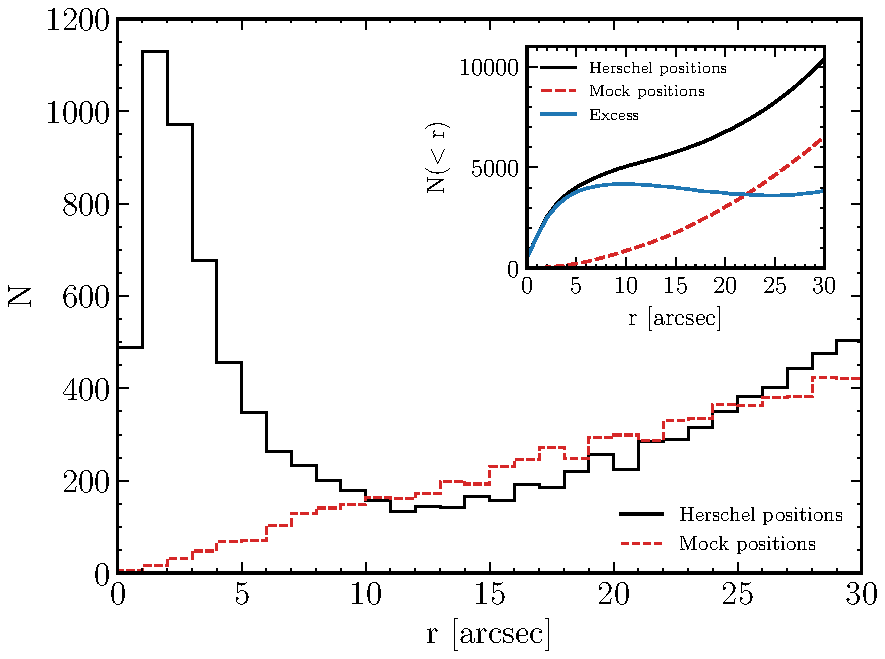
\includegraphics[width=0.75\columnwidth]{Figures/optimal_radius.pdf}
	\caption{{\color{red} Caption.}}
	\label{fig:optimal_radius}
\end{figure}

Given that our VLA observations have a surface density of $4103\,$deg$^{-2}$ and we are assuming a maximum search radius of 10\,arcsec, we can approximate the maximum value of $P$. As a first order approximation, the maximum $P$ value is equal to the ratio between the probability of observing at least one VLA source within the search radius of a random position and the probability that the position is a blank field. Assuming Poisson statistics with a mean number of counterparts per random position of $\lambda = N_{\textrm{VLA}}A_{\textrm{random}}/A_{\textrm{survey}}$, where $N_{\textrm{VLA}}$ is the number of VLA sources, $A_{\textrm{random}}$ is the search area around a random position and $A_{\textrm{survey}}$ is the total survey area, then an estimate of $P_{\textrm{max}}$ can be given by:

\begin{equation}
    P_{\textrm{max}} \approx \frac{P(\textrm{Not Blank})}{P(\textrm{Blank})} = \frac{P(X > 0)}{P(X = 0)} = \frac{1 - P(X = 0)}{P(X = 0)} = \frac{1 - e^{-\lambda}}{e^{-\lambda}} \approx 0.10,
\end{equation}

\noindent where $X$ is the number of VLA sources observed around each random position. This calculation suggests that the maximum $P$ value for any radio source observed near a \textit{Herschel} source is $0.1$, not considering effects such as clustering, multicomponent galaxies or overlapping search areas. The fact that only $\sim$ 10\% of random positions will be incident with at least one radio source gives further confidence in the association between any \textit{Herschel} and VLA sources in close proximity.

\section{Results of the Frequentist Method Applied to \textit{Herschel} Sources}

We apply the method described above to all possible VLA counterparts within 10\,arcsec of a SPIRE source. We retain all counterparts that have $P < 0.05$, but consider as our primary counterparts those with the lowest $P$ value per \textit{Herschel} source. Figure \ref{fig:ds_distributions} shows the distribution of $S$ for radio counterparts to \textit{Herschel} (black histogram) and $10^6$ random positions (red histogram). The clear offset between the two distributions illustrates how a large fraction of the counterparts identified in the radio trace the sub-mm sources.

\begin{figure}
	\centering
	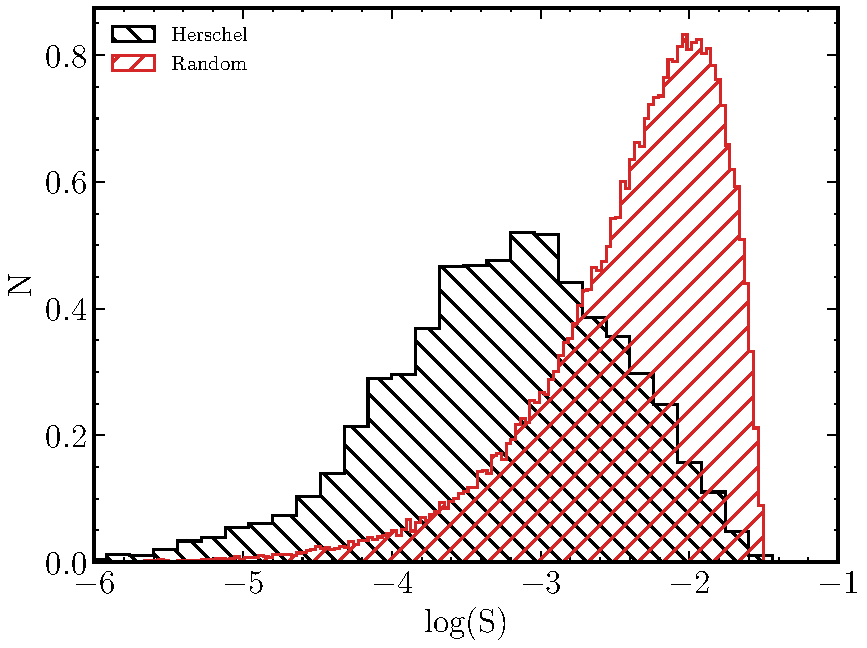
\includegraphics[width=0.75\columnwidth]{Figures/ds_distributions.pdf}
	\caption{{\color{red} Caption.}}
	\label{fig:ds_distributions}
\end{figure}

The total identification rate, that is the number of sources identified with $P < 0.05$ by a radio source, is 3,787/7,230 (52\%). However, the identification rate is a strong function of the sub-mm flux density (Figure \ref{fig:id_rate}). There is a strong decline toward fainter 250\,\micron\ fluxes ($< 30\,$mJy) where we approach the confusion limit of the survey. To be consistent with our motivation for a clean and unambiguous sample of \textit{Herschel} galaxies and their multiwavelength properties, we henceforth refer only to the sources with 250\,\micron\ flux densities greater than 30\,mJy, where we are more confident that they correspond to true sources. The survey area corresponds to 1,324 \textit{Herschel} sources with $S_{250\,\mu m} > 30\,$mJy. Of these sources, 1,053 (80\%) have radio IDs with $P < 0.05$.

\begin{figure}
	\centering
	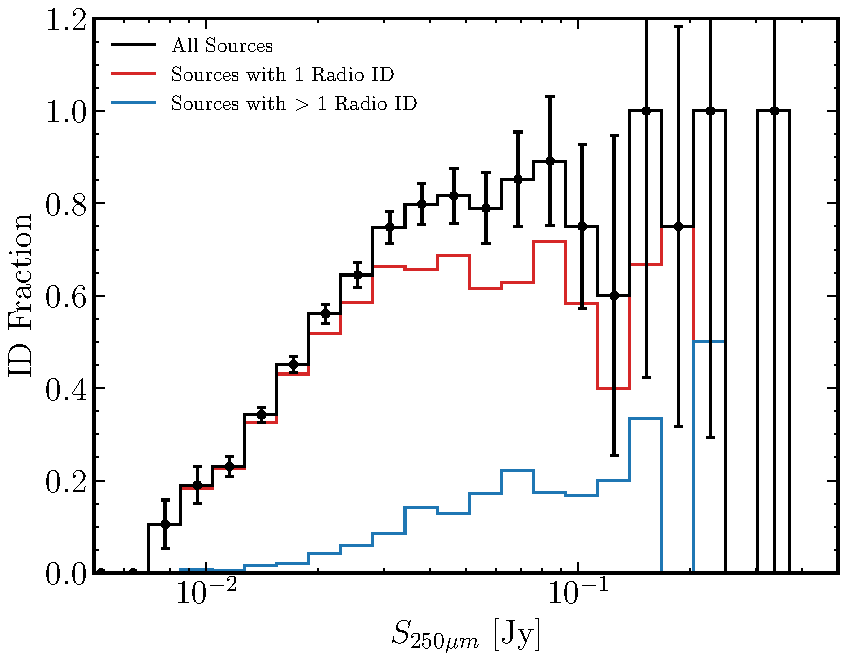
\includegraphics[width=0.75\columnwidth]{Figures/id_fraction_radio.pdf}
	\caption{{\color{red} Caption.}}
	\label{fig:id_rate}
\end{figure}

Given that $P_i$ represents the probability of observing a radio counterpart, $i$, with a given flux and offset from the source by chance, the number of false IDs in a $P$-limited sample is given by

\begin{equation}
    N_{\textrm{False}} = \sum_{P_i < 0.05} P_i,
    \label{eq:false_radio_ids}
\end{equation}

\noindent which is analogous to Equation \ref{eq:false_ids} when using the LR method. From this we estimate that the false identification rate is approximately 0.5\% ($N_\textrm{False} \approx 7$). Compared to the fraction of false reliable counterparts identified in the near-IR as part of the H-ATLAS SGP ($\sim$ 4.8\%), the cleanness of the radio sample appears to be much higher. One of the driving factors of this difference is the surface density of radio sources compared to near-IR galaxies. The average number of potential counterparts per source for the VIKING analysis was $\sim 5.2$ (1,005,359 counterparts to 193,527 sources), which if we scale to a search radius of 10\,arcsec reduces to $\sim 2.1$ assuming they are uniformly scattered across the survey. By comparison, there are approximately 1.5 radio sources for each \textit{Herschel} source in COSMOS (10,826 counterparts to 7,230 sources).

While the above estimate of the false ID rate was computed for those counterparts with the lowest value of $P$ per source (the "primary" sample), we also observe secondary and tertiary associations that also have $P < 0.05$. For the 1,053 sub-mm sources that have robust identifications, 879 (83.5\%) have just a single association, 160 (15.2\%) have two and 14 (1.3\%) have three. The straightforward interpretation of single counterparts is that the radio source is the sole location of the far-IR emission. This is further supported if the counterpart is especially bright and close to the source, this would suggest that we are not likely to be mistaken by confusion or by larger offsets that may suggest missing secondaries that are below our detection. However, the nature of the multiple systems is less obvious and is explored in Section \ref{sec:multiple_systems}.

{\color{red}Talk about the crossmatching with COSMOS2020 so we can talk about i) redshift distribution.}

\subsection{Positional Errors and the \textit{Herschel}-SPIRE Point Spread Function}

The excellent accuracy of the 3\,GHz VLA sources (angular resolution of 0.75\,arcsec) means that the distribution of the offsets between the source position and the counterparts can be assumed to be an approximation of the sub-mm positional errors. As demontrated in Chapter \ref{chapter:Data_Release_3}, the \textit{Herschel}-SPIRE point spread function (PSF) is often assumed to take the form of a Gaussian, which we have previously estimated to have a width of $\sigma \sim 2.4$\,arcsec. In the following we use our set of robust radio identifications to validate this claim.

Figure \ref{fig:source_counterpart_offset} shows the positional offsets for the radio data from the sub-mm location. The solid line shows the offsets for all primary counterparts, the dotted line for all associations including secondaries and tertiaries, and the dashed line shows the average offset of all radio counterparts for each \textit{Herschel} source. On the assumption of Gaussian errors in R.A. and Dec, and if the distribution of radial offsets truly originates from random uncertainties in the position of the sub-mm source, then the distribution of radial offsets should resemble a Rayleigh distribution of the form $R(r, \sigma) \propto \frac{r}{\sigma^2}e^{-\frac{r^2}{2\sigma^2}}$. This results from the fact that for two independent Gaussian random variables with mean zero and standard deviation $\sigma$, as we might expect for the offset in R.A. and Dec ($\Delta\alpha$, $\Delta\delta$), then the offset defined as $r = \sqrt{\Delta\alpha^2 + \Delta\delta^2}$ has a Rayleigh distribution with parameter $\sigma$. The distribution of positional offsets from the sub-mm position for the primary radio sources is well described by a Rayleigh distribution with a width $\sigma = 1.66\,$arcsec (red line). This is substantially lower than our estimate of the 1$\sigma$ positional error measured in Chapter \ref{chapter:Data_Release_3} ($\sigma_{\textrm{pos}} = 2.388\pm0.065$\,arcsec). The corresponding Rayleigh distribution with $\sigma = 2.388$ for the same number of counterparts is illustrated with the green line in Figure \ref{fig:source_counterpart_offset}. This represents the expected distribution of radio offsets assuming the form of the source positional errors, $f(r)$, that is typically used in previous \textit{Herschel}-ATLAS studies (we refer the reader to Figure \ref{fig:Q_estimate}). However, we are reminded that our estimate of $\sigma_{\textrm{pos}}$ from the LR method relied on counting the number of blank sub-mm positions observed on the near-IR images, which is much shallower than the radio data used here. The median redshift of our near-IR counterparts was $\sim 0.49$, while the median redshift of our radio detected sample is $\sim 0.91$. By scaling the value of $\sigma_{\textrm{pos}}$ by the physical distance this corresponds to at the median redshift of the radio IDs, we predict that the positional error should be $\sigma_{\textrm{pos}} \sim 1.85$. The rescaled Rayleigh distribution is illustrated as the dashed green line. We see that this expected distribution is in much better agreement with our measurement of the positional errors. This suggests that in the absence of any knowledge of the sub-mm positional error distribution, the LR method retrieves a reasonable function for $f(r)$ that mostly resembles the distribution we observe from astrometrically precise radio positions.

\begin{figure}
	\centering
	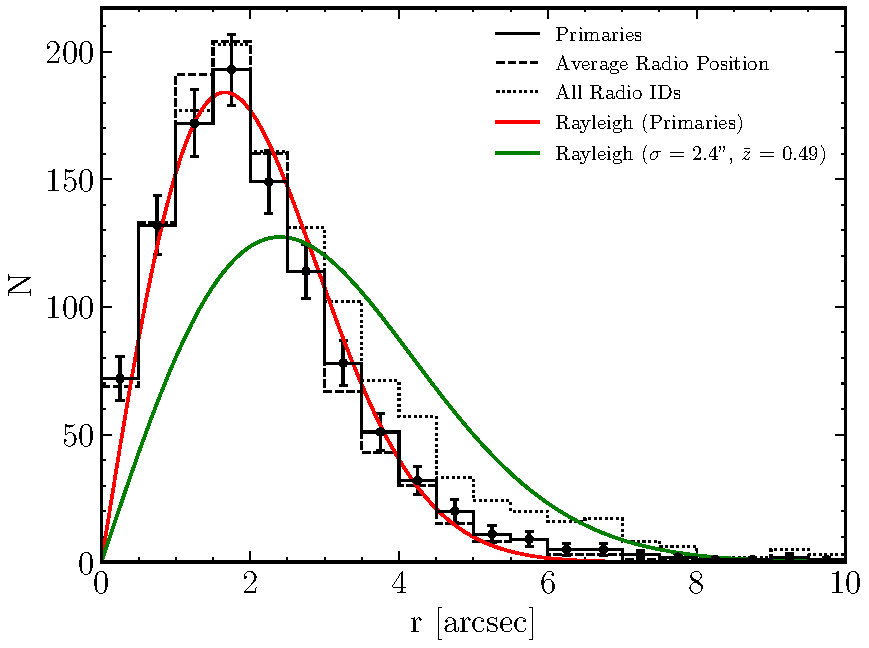
\includegraphics[width=0.75\columnwidth]{Figures/source_counterpart_offsets.pdf}
	\caption{{\color{red} Caption.}}
	\label{fig:source_counterpart_offset}
\end{figure}

\subsection{The Nature of Multiple Identifications}
\label{sec:multiple_systems}

For roughly one sixth of sources, the correct identification is not obvious due to secondary and possibly tertiary candidates with a low probability of occurring by chance. There are several interpretations of such multiplicity. One possible explanation is that the radio sources are gravitationally lensed images of the far-IR emitting galaxy, but as mentioned earlier, this is unlikely. Other possibilities include clustering of true associations or unrelated counterparts that are flux boosted in the sub-mm by confusion noise. Determining unambiguously whether \textit{Herschel} sources with multiple identifications are predominantly physically associated or the result of confusion would require spectroscopic data. A number of studies have suggested that SMGs are strongly clustered (e.g. \citealt{Blain_2004}; \citealt{Weiss_2009}) while other studies suggest that multiple associations can be explained solely by the low angular resolution of single-dish observations (e.g. \citealt{Williams_2011}). Studies using interferometric observations at millimeter wavelengths have already shown that $\gtrsim$ 20\% of sub-mm sources correpsond to multiple SMGs that have been blended in single-dish observations (\citealt{Karim_2013}; \citealt{Simpson_2015}; \citealt{Stach_2018}). 

We attempt to understand the nature of our multiple systems by considering two questions: i) are all multiple counterparts to a source real? ii) are the counterparts, if physical, associated with each other? First, we note that the ID fraction of sources with multiple counterparts (Figure \ref{fig:id_rate}) is not restricted to low 250\,\micron\ flux densities, suggesting that most of the sources are real and thus their multiplicity is a product, either directly or indirectly, of a real sub-mm source. The ID fraction increases with flux density, which is not surprising since the inclusion of emission from multiple SMGs will only increase the total flux. The fractional contribution of the brightest radio ID to the total 3\,GHz flux density is plotted as a function of the 250\,\micron\ source flux density in the top panel of Figure \ref{fig:multiples_flux_contribution}. The median and standard deviation in the distribution of fractional contributions to the total 3\,GHz flux density is shown by the black error bars for the brightest radio component, and as red and blue lines for the second and third components, respectively. Some sources appear to have radio components where one counterpart dominates the radio flux ($\gtrsim 90\%$). In these cases we may presume that the sub-mm source corresponds to the bright radio object thanks to the well defined far-IR/radio correlation, and the minor components can effectively be ignored (or are chance background sources). However, the majority of our brightest counterparts contribute $\sim 50 - 70\%$ with significant contributions coming from secondary and possibly tertiary associations. The interpretation here is that the sub-mm emission emanates from more than one SMG that have been blended together by the \textit{Herschel}-SPIRE beam.

\begin{figure}
	\centering
	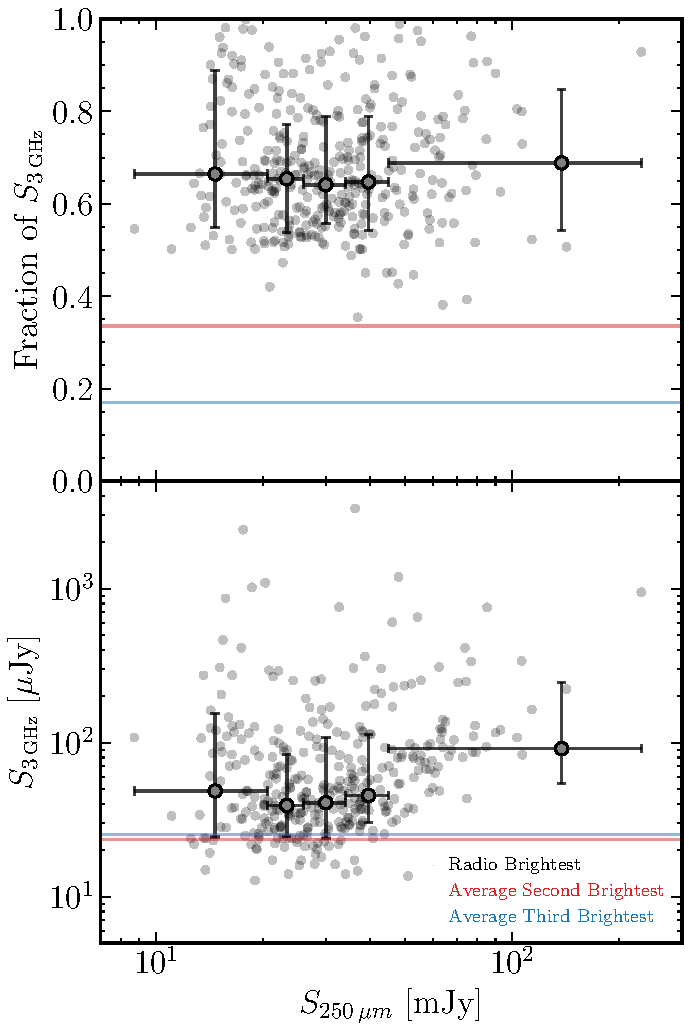
\includegraphics[width=0.75\columnwidth]{Figures/multiples_flux_contribution.pdf}
	\caption{{\color{red} Caption.}}
	\label{fig:multiples_flux_contribution}
\end{figure}

There appears to be no dependence of the median flux fraction of the brightest component on the total 250\,\micron\ flux. Previous studies (e.g. \citealt{Scudder_2016}) have suggested that the fractional contribution increases toward low source flux density, but there is only weak evidence here. The bottom panel of Figure \ref{fig:multiples_flux_contribution} shows the raw flux of all the brightest components as a function of the total 250\,\micron\ flux density. 

\subsection{Missing Identifications}



\chapter{Conclusion}
\label{chapter:Conclusion}
\chapquote{``A quote"}{By whom}{From what source}

\section{Thesis Overview}
\section{Key Results}
\section{Future work}
\section{Concluding remarks}

\listoftodos

\appendix


\titleformat{\chapter}[display]{}{}{0pt}{{\textbf \huge \textsc{Appendix} \thechapter}\\ \huge \textbf \textsc}[\titlerule\vspace{2pt}\titlerule]

\chapter{Candidate Lensed Sources in the SGP ($S_{\textrm{500\,\micron}}$ > 100\,mJy)}


\label{app:candidate_lenses_bright}

\chapter{HerBS Sample Photometry}

\begin{landscape}
\begin{longtable}{lccccccccccr}

	\caption{Spectroscopic redshifts, lensing magnifications and photometry for HerBS sources.}
	\label{tab:data_herbs} \\
	\hline
	\hline
	Source & Spec-z & $\mu$ & $S_{250\,\micron}$ & $S_{350\,\micron}$ & $S_{500\,\micron}$ & $S_{850\,\micron}$ & $S_{1.2\,\textrm{mm}}$ & $S_{2\,\textrm{mm}}$ & $S_{3\,\textrm{mm}}$ \\
    & & & (mJy) & (mJy) & (mJy) & (mJy) & (mJy) & (mJy) & (mJy) \\
	\hline
    \hline
	HerBS-11 & 2.631 & 18.4 & 257.5$\pm$6.4 & 271.1$\pm$6.3 & 204.0$\pm$7.2 & 67.3$\pm$6.3 & -- & 3.59$\pm$0.03 & 0.93$\pm$0.02\\
	HerBS-14 & 3.782 & 36.4 & 116.3$\pm$6.1 & 177.0$\pm$6.3 & 179.3$\pm$7.5 & 77.9$\pm$6.4 & 28.9$\pm$0.6 & 7.31$\pm$0.04 & 1.50$\pm$0.02\\
	HerBS-18 & 2.182 & 27.9 & 212.9$\pm$4.7 & 244.2$\pm$5.0 & 169.4$\pm$6.2 & 52.9$\pm$6.1 & -- & 2.73$\pm$0.03 & 0.74$\pm$0.06\\
	HerBS-21 & 3.323 & 6.1 & 125.8$\pm$5.5 & 185.5$\pm$5.8 & 155.1$\pm$7.4 & 51.3$\pm$6.3 & -- & 3.92$\pm$0.03 & 0.94$\pm$0.10\\
	HerBS-24 & 2.198 & 4.6 & 170.9$\pm$5.7 & 197.1$\pm$6.3 & 145.6$\pm$7.4 & 64.8$\pm$7.8 & -- & 2.68$\pm$0.03 & 0.74$\pm$0.03\\
	HerBS-25 & 2.912 & 49.8 & 112.5$\pm$5.0 & 148.0$\pm$5.4 & 143.4$\pm$6.5 & 49.2$\pm$5.7 & -- & 3.52$\pm$0.03 & 0.81$\pm$0.11\\
	HerBS-27 & 4.509 & 14.6 & 72.2$\pm$5.3 & 129.8$\pm$5.6 & 138.6$\pm$7.0 & 90.5$\pm$6.3 & 28.9$\pm$1.0 & 8.70$\pm$0.03 & 1.97$\pm$0.02\\
	HerBS-28 & 3.925 & 5.7 & 79.4$\pm$5.8 & 135.4$\pm$6.0 & 140.0$\pm$7.4 & 79.4$\pm$7.8 & 25.5$\pm$1.2 & 5.56$\pm$0.03 & 1.66$\pm$0.10\\
	HerBS-36 & 3.095 & 5.4 & 121.5$\pm$6.1 & 161.0$\pm$6.7 & 125.5$\pm$7.7 & 64.0$\pm$8.8 & -- & 4.81$\pm$0.03 & 1.11$\pm$0.02\\
	HerBS-39 & 3.229 & 5.1 & 118.3$\pm$5.1 & 141.2$\pm$5.5 & 119.7$\pm$6.8 & 36.5$\pm$7.0 & -- & 3.01$\pm$0.03 & 0.64$\pm$0.03\\
	HerBS-41 & 4.098 & 2.1 & 63.3$\pm$6.2 & 91.1$\pm$6.1 & 121.7$\pm$7.4 & 31.8$\pm$5.9 & 15.2$\pm$0.5 & 4.85$\pm$0.07 & --\\
	HerBS-42 & 3.307 & 3.9 & 130.3$\pm$5.8 & 160.0$\pm$6.1 & 116.2$\pm$6.8 & 50.4$\pm$6.1 & -- & 2.95$\pm$0.06 & 0.58$\pm$0.05\\
	HerBS-49 & 2.727 & 15.3 & 76.8$\pm$6.0 & 110.9$\pm$6.2 & 110.4$\pm$7.3 & 31.9$\pm$8.5 & -- & 1.69$\pm$0.04 & 1.13$\pm$0.09\\
	HerBS-55 & 2.656 & 13.7 & 109.0$\pm$5.3 & 116.5$\pm$5.5 & 107.1$\pm$6.6 & 29.9$\pm$7.1 & -- & 1.05$\pm$0.03 & 0.33$\pm$0.02\\
	HerBS-57 & 3.265 & 15.0 & 118.1$\pm$4.9 & 147.3$\pm$5.2 & 105.4$\pm$6.4 & 60.7$\pm$8.5 & -- & 3.05$\pm$0.02 & 0.50$\pm$0.02\\
	HerBS-60 & 3.261 & 9.5 & 73.3$\pm$5.8 & 101.2$\pm$6.1 & 103.6$\pm$7.5 & 39.8$\pm$5.7 & 13.2$\pm$0.8 & 2.54$\pm$0.03 & 0.53$\pm$0.02\\
	HerBS-68 & 2.719 & 10.5 & 139.1$\pm$5.3 & 144.8$\pm$5.4 & 100.5$\pm$6.6 & 46.7$\pm$7.7 & -- & 1.62$\pm$0.04 & 0.32$\pm$0.05\\
	HerBS-73 & 3.026 & 3.1 & 117.1$\pm$6.0 & 129.0$\pm$6.2 & 99.6$\pm$7.4 & 49.4$\pm$6.8 & -- & 2.09$\pm$0.03 & 0.43$\pm$0.02\\
	HerBS-86 & 2.564 & 4.8 & 77.4$\pm$5.6 & 90.7$\pm$5.8 & 96.0$\pm$7.4 & 33.8$\pm$6.1 & 8.1$\pm$0.6 & 1.56$\pm$0.02 & 0.25$\pm$0.02\\
	HerBS-93 & 2.400 & 2.4 & 77.3$\pm$5.4 & 87.3$\pm$5.7 & 94.8$\pm$7.0 & 22.8$\pm$5.7 & 6.2$\pm$0.4 & 1.39$\pm$0.02 & 0.16$\pm$0.01\\
	HerBS-103 & 2.942 & 4.3 & 126.1$\pm$5.3 & 131.2$\pm$5.7 & 93.5$\pm$7.0 & 33.7$\pm$7.6 & -- & 1.40$\pm$0.03 & 0.42$\pm$0.02\\
	HerBS-111 & 2.371 & 4.3 & 105.9$\pm$6.5 & 115.6$\pm$6.2 & 92.7$\pm$7.4 & 13.3$\pm$6.9 & -- & 1.13$\pm$0.02 & 0.21$\pm$0.02\\
	HerBS-132 & 2.473 & 4.8 & 86.7$\pm$5.8 & 102.6$\pm$6.0 & 90.6$\pm$7.8 & 16.6$\pm$7.4 & -- & 0.86$\pm$0.02 & 0.16$\pm$0.02\\
	HerBS-145 & 2.730 & 1.9 & 54.7$\pm$6.0 & 67.4$\pm$6.2 & 86.8$\pm$7.7 & 13.4$\pm$7.0 & 5.1$\pm$0.6 & 1.06$\pm$0.04 & --\\
	HerBS-160 & 3.955 & 8.1 & 48.6$\pm$5.6 & 84.2$\pm$6.0 & 84.8$\pm$7.1 & 36.6$\pm$6.4 & 15.0$\pm$0.6 & 3.94$\pm$0.02 & 0.91$\pm$0.02\\
	HerBS-182 & 2.227 & 1.1 & 89.0$\pm$5.7 & 109.1$\pm$6.2 & 82.3$\pm$7.9 & -- & -- & 1.04$\pm$0.03 & 0.21$\pm$0.02\\
	HerBS-184 & 2.507 & 6.0 & 91.9$\pm$5.9 & 107.6$\pm$6.0 & 82.3$\pm$7.1 & -- & -- & 1.49$\pm$0.02 & 0.48$\pm$0.02\\
	HerBS-200 & 2.151 & 0.4 & 107.1$\pm$6.1 & 109.7$\pm$6.0 & 80.5$\pm$7.5 & 11.3$\pm$6.6 & -- & 0.78$\pm$0.02 & 0.25$\pm$0.01\\
	HerBS-207 & 1.569 & 5.2 & 96.9$\pm$5.9 & 121.7$\pm$6.1 & 80.2$\pm$7.5 & 33.1$\pm$6.3 & -- & 0.89$\pm$0.02 & 0.25$\pm$0.03\\
	HerBS-208 & 2.481 & 1.4 & 69.4$\pm$5.1 & 91.9$\pm$5.5 & 80.1$\pm$6.6 & -- & -- & 1.40$\pm$0.05 & 0.32$\pm$0.04\\
	\hline
\end{longtable}
\end{landscape}

\label{app:HerBS_photometry}

\chapter{SPT-DSFG Sample Photometry}


\label{app:SPT_DSFG_photometry}

\chapter{HerBS SEDs}

\begin{figure}
	\centering
	\includegraphics[width=\columnwidth]{Figures/herbs_ot_SEDs.pdf}
	\caption{Caption.}
\end{figure}

\begin{figure}
	\centering
	\includegraphics[width=\columnwidth]{Figures/herbs_go100_SEDs.pdf}
	\caption{Caption.}
\end{figure}

\begin{figure}
	\centering
	\includegraphics[width=\columnwidth]{Figures/herbs_go200_SEDs.pdf}
	\caption{Caption.}
\end{figure}
\label{app:HerBS_SEDs}

\chapter{SPT-DSFG SEDs}


\label{app:SPT_DSFG_SEDs}

% Define bibliography
\titleformat{\chapter}[display]{}{}{0pt}{\huge \textbf \textsc}[\titlerule\vspace{2pt}\titlerule]
%\input{journalCommand}


%\printbibliography
\bibliographystyle{mnras}
\bibliography{Thesis.bib}

%% Uncomment \layout* to view layout config page
% \layout*
\end{document}